\documentclass[11pt]{article}
\usepackage{amsmath,amssymb,amsfonts,latexsym,xspace,amsthm,array,float}
\usepackage[utf8]{inputenc}
\usepackage{a4wide,hyperref}
\usepackage[lined,boxed,commentsnumbered]{algorithm2e}
\usepackage{tikz}
\usepackage{wrapfig}
\usetikzlibrary{patterns}
\usepackage[final]{showkeys}

\newenvironment{pf}{{\em \noindent Proof:}}{ \hfill \qed\smallskip}

\tikzstyle{Grisfill}=[fill=black!10]
\colorlet{darkgreen}{green!50!black}
\colorlet{darkred}{red!50!black}

\tikzstyle{H}=[red]
\tikzstyle{Hfill}=[fill=red!20]
\tikzstyle{Hpoint}=[fill=darkred,darkred]

\tikzstyle{V}=[green]
\tikzstyle{Vfill}=[fill=green!20]
\tikzstyle{Vpoint}=[darkgreen,fill=darkgreen]

\definecolor{vert}{rgb}{0,0.75,0.25}
\newcommand{\R}{\ensuremath{\color{red}R}\xspace}
\newcommand{\G}{\ensuremath{\color{vert}G}\xspace}

\newcommand{\RRR}{\ensuremath{\color{red}132}\xspace}
\newcommand{\GGR}{\ensuremath{{\color{vert}1}{\color{red}X}{\color{vert}2}}\xspace}
\newcommand{\RRG}{\ensuremath{{\color{vert}2}/{\color{red}1}{\color{red}3}}\xspace}
\newcommand{\GGG}{\ensuremath{\color{vert}213}\xspace}





\makeatletter
\newcommand{\rmnum}[1]{\romannumeral #1}
\newcommand{\Rmnum}[1]{\expandafter\@slowromancap\romannumeral #1@}
\makeatother

\newcommand{\Vpoint}[2]{\draw (#1,#2) [darkgreen,fill=darkgreen] circle (3pt);}
\newcommand{\Hpoint}[2]{\draw (#1,#2) [darkred,fill=darkred] circle (3pt);}
\newcommand{\zoneD}[1]{\draw [#1,#1fill, very thick] (4,0) -- (5,0) -- (5,1) -- (4,1);}
\newcommand{\zoneE}[1]{\draw [#1,#1fill, very thick] (5,0) -- (6,0) -- (6,1) -- (5,1) -- (5,0);}
\newcommand{\zoneB}[1]{\draw [#1,#1fill, very thick] (5,-1) -- (5,0) -- (6,0) -- (6,-1);}
\newcommand{\zoneF}[1]{\draw [#1,#1fill, very thick] (7,1) -- (6,1) -- (6,0) -- (7,0);}
\newcommand{\zoneH}[1]{\draw [#1,#1fill, very thick] (5,2) -- (5,1) -- (6,1) -- (6,2);}
\newcommand{\zoneA}[1]{\draw [#1,#1fill, very thick] (5,-1) -- (5,0) -- (4,0);}
\newcommand{\zoneC}[1]{\draw [#1,#1fill, very thick] (6,-1) -- (6,0) -- (7,0);}
\newcommand{\zoneG}[1]{\draw [#1,#1fill, very thick] (4,1) -- (5,1) -- (5,2);}

\newcommand{\Hzone}{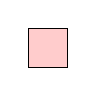
\begin{tikzpicture}[scale=.5]
\draw [Hfill] (0,0) rectangle (1,1); 
\end{tikzpicture}~}
\newcommand{\Vzone}{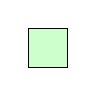
\begin{tikzpicture}[scale=.5]
\draw [Vfill] (0,0) rectangle (1,1); 
\end{tikzpicture}~}

\newcommand{\zoneRG}[3]{
\draw [very thick,H,Hpoint] (#1,#2) -- +(-#3,0);
\draw [very thick,V,Vpoint] (#1,#2) -- +(0,#3);
\draw [Hfill] (#1,#2) -- +(-#3,#3) -- +(-#3,0);
\draw [Vfill] (#1,#2) -- +(-#3,#3) -- + (0,#3);
}
\newcommand{\zoneGR}[3]{
\draw [very thick,H,Hpoint] (#1,#2) -- +(-#3,0);
\draw [very thick,V,Vpoint] (#1,#2) -- +(0,#3);
\draw [Vfill] (#1,#2) -- +(-#3,#3) -- +(-#3,0);
\draw [Hfill] (#1,#2) -- +(-#3,#3) -- + (0,#3);
}


\newcommand{\zoneI}[1]{\draw [#1,#1fill, very thick] (6,2) -- (6,1) -- (7,1);}
\newcommand{\etiquette}[1]{\draw (2.5,1) node {(\rmnum{#1})};}

\newtheorem{thm}{Theorem}[section]
\newtheorem{prop}[thm]{Proposition}
\newtheorem{rem}[thm]{Remark}
\newtheorem{defn}[thm]{Definition}
\newtheorem{lem}[thm]{Lemma}
\newtheorem{csq}[thm]{Consequence}

\newcommand{\C}{\ensuremath{\mathcal C}}

\newcommand{\patternV}{\ensuremath{|12|\ |}\xspace}
\newcommand{\patternH}{\ensuremath{|\ |132|}\xspace}
\newcommand{\patternVH}{\ensuremath{|2|13|}\xspace}


\newcommand{\pushall}{-stack pushall sortable\xspace}
\newcommand{\ssi}{if and only if\xspace}
\newcommand{\ascentRG}{increasing sequence \xspace}
\newcommand{\ascentGR}{increasing sequence \xspace}
\newcommand{\ascentRR}{increasing sequence \xspace}
\newcommand{\ascentGG}{increasing sequence \xspace}
\newcommand{\ascentsRG}{increasing sequences \xspace}
\newcommand{\ascentsGR}{increasing sequences \xspace}



\newcounter{indice}

\newcommand{\permutation}[1]{
\setcounter{indice}{0};
\foreach \i in {#1} 
\addtocounter{indice}{1};

\addtocounter{indice}{1}
\draw [help lines] (1,1) grid (\theindice,\theindice);

\setcounter{indice}{1};

\foreach \i in { #1 } {
\draw (\theindice+.5,\i+.5) [fill] circle (.2);
\addtocounter{indice}{1};
}
\addtocounter{indice}{-1};
}



\title{\pushall permutations \footnote{This work was completed with the support of the ANR
   project ANR BLAN-0204\_07  MAGNUM}}
\author{Adeline Pierrot \and Dominique Rossin}

\begin{document}
\maketitle
\begin{abstract}
In the 60's, Knuth introduced stack-sorting and serial compositions of stacks.
In particular, one significant question arise out of the work of Knuth: 
how to decide efficiently if a given permutation is sortable with  stacks in series?
Whether this problem is polynomial or \mbox{NP-complete} is still unanswered yet.
In this article we introduce -stack pushall permutations which form a subclass of -stack sortable permutations 
and show that these two classes are closely related. 
Moreover, we give an optimal  algorithm to decide if a given permutation of size  is \pushall and describe all its sortings.
This result is a step to the solve the general -stack sorting problem in polynomial time.
\end{abstract}

\section{Introduction}

In the 60's, Knuth introduced the problem of stack-sorting \cite{Knuth68} and 
then serial compositions of stacks \cite{Knuth73}.
To answer the one-stack case, he introduced both the pattern-containment relation on permutations and permutation classes, two new fields of combinatorics. 
Stack-sorting was further generalized to sorting networks by Tarjan \cite{Tarjan72}
while several variants appear by either considering other types of combinatorial structures or by changing rules \cite{Pratt73,EvenItai71,AAL10}.

In this article, we focus on sorting with two stacks in series. 
More precisely, if  is a permutation, we consider  as a sequence of integers  that we take as input
and at each step we have three possibilities as described in Figure~\ref{fig:rholambdamu} (p.\pageref{fig:rholambdamu}):
\begin{enumerate}
\item[:] Get the next element of  and push its value on top of the first stack denoted .
\item[:] Pop the topmost element of stack  and push this value on top of the second stack .
\item[:] Pop the topmost element of  and write it to the output.
\end{enumerate}

We iterate over these three possibilities until all elements have been output. 
If there is a sequence of operations that leads to identity on the output, 
then we say that the permutation is -stack sortable. 
Three natural questions among others arise:
\begin{enumerate}
\item Decision: what is the complexity of the problem consisting of deciding whether a given permutation is sortable or not?
\item Characterization: can one characterize permutations that are sortable?
\item Counting: establish the generating function of sortable permutations.
\end{enumerate}

For the one-stack case these three problems were solved by Knuth in \cite{Knuth68}. 
A greedy algorithm allows to answer the decision problem in linear time. 
Moreover he characterized sortable permutations by introducing the -avoiding permutations class, 
whose generating function is the Catalan series. 
Since this article, the more general question of sorting with multiple stacks in series or in parallel has been widely studied.
Knuth \cite{Knuth68}, Tarjan \cite{Tarjan72} and Pratt \cite{Pratt73} noted that the permutations sortable by the various configurations 
could be described by forbidding certain patterns to occur in the permutations.

Regarding  parallel stacks,
the decision problem can be answered in time  for ,
while for  this is NP-complete (this is proved by a reduction in~\cite{EvenItai71} to a problem solved in~\cite{Unger92}).
The characterization problem is studied in~\cite{Pratt73}:
for , the basis of the class of permutations sortable with  stacks in parallel is infinite.
Finally, about the counting problem,
when  the generating function is described in \cite{ABM}, but by an infinite system of equations.



For stacks in series, it has been shown in \cite{Knuth68} that every permutation of size  can be sorted by  stacks in series. 
But none of the above three questions has been answered for more than one stack in series. 
For two stacks, Murphy \cite{Murphy02} proved that the basis of the class of sortable permutations is infinite. 
In his Phd thesis, he also studies the problem of deciding whether a given permutation is sortable with  stacks in series.
He reduced this problem to a -SAT problem;
at the same time he reduced a -SAT instance to the decision problem,
and hoped than one of both reduction was actually an equivalence.
But none of those results has been proved or disproved. 
In \cite{Bona02}, B\'ona gives an overview of advances in sorting networks and mentions this problem as possibly NP-complete.
More surprising, both conjectures exist:
in \cite{AMR02b}, the authors conjectured that the decidability problem is NP-complete,
while Murphy in his PhD (\cite{Murphy02} Conjecture 260) conjectured that it is in .
Several weaker variants of this problem have been studied. 
First, West considered permutations sortable with two consecutive greedy passes through a stack in \cite{West90, West93}. 
He conjectured the enumeration formula which was proved after by Zeilberger \cite{Zeilberger92}. 
For more than two passes, few results are known~\cite{BM00, Ulfarsson11}. 
Another variant studied in~\cite{AMR02b} is to consider decreasing stacks (i.e.~elements in the stack must be decreasing from bottom to top)
instead of general stacks.
In this article we define a new restriction of -stacks sorting, namely -stacks pushall sorting,
and prove that the decidability problem in this case is polynomial.

\bigskip
Throughout this article we usually write permutations as  
where  is the size of , denoted by , and  is the image of  for all . 
A permutation  is a {\em pattern} of  if and only if there exist 
 such that  is order isomorphic to . 
We note  the set of permutations avoiding , i.e.~not having any permutation of  as a pattern.
A {\em permutation class}  is a set of permutations downward-closed for the pattern relation: 
if  belongs to , then every pattern of  belongs to . 
Note that for any set ,  is a class.
A permutation class  can be defined by its minimal set  such that .
This minimal set is called the {\em basis} of the class. 
For example, Knuth proved that -stack sortable permutations are those that belong to the class .
Unfortunately, the basis can be infinite. 
For -stack sortable permutations, as stated above, it has been proved in~\cite{Murphy02} that the basis is infinite.

A permutation can also be represented by its
{\it diagram}, consisting in the set of points at coordinates  drawn in the plane
(see two examples in Figure~\ref{fig:graphicalRepresentation}).
An {\em interval} in a permutation is a consecutive range of elements, consecutive both in indices and values. 
For example in the permutation , the elements  form an interval: 
they are consecutive in the permutation and the values span the whole integer interval . 
In the diagram, note that an interval is a square
which is itself a diagram of a permutation (if translated to the origin).
In particular, no point outside this square has the same x or y coordinate than any cell of the square
(see the yellow stripes of Figure~\ref{fig:graphicalRepresentation}).
A permutation where all intervals are trivial --either a singleton or the whole permutation-- is called a {\em simple} permutation. 
For instance,  and  are the two simple permutations of size .
An {\em inflation} of an element  in  by a permutation  is the permutation obtained 
by replacing  by  and renormalizing the resulting permutation. 
For example if we inflate  in  by the permutation , 
we obtain the permutation 
(see the second diagram of Figure~\ref{fig:graphicalRepresentation}).
Notice that in an inflation by , elements corresponding to  form an interval in the resulting permutation.

\begin{figure}[H]
\begin{center}
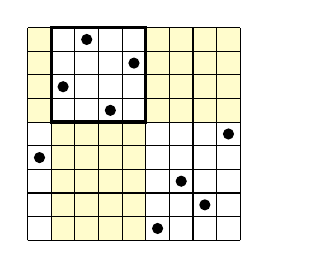
\begin{tikzpicture}[scale=.3]
\useasboundingbox (0,0) rectangle (11,9);
\fill [color=yellow!20!white] (0,5) rectangle +(1,4);
\fill [color=yellow!20!white] (1,0) rectangle +(4,5);
\fill [color=yellow!20!white] (5,5) rectangle +(4,4);
\draw[thin] (0,0) grid (9,9);
\draw[fill] (.5,3.5) circle (6pt);
\draw[fill] (1.5,6.5) circle (6pt);
\draw[fill] (2.5,8.5) circle (6pt);
\draw[fill] (3.5,5.5) circle (6pt);
\draw[fill] (4.5,7.5) circle (6pt);
\draw[fill] (5.5,0.5) circle (6pt);
\draw[fill] (6.5,2.5) circle (6pt);
\draw[fill] (7.5,1.5) circle (6pt);
\draw[fill] (8.5,4.5) circle (6pt);
\draw [very thick] (1,5) rectangle +(4,4);
\end{tikzpicture}
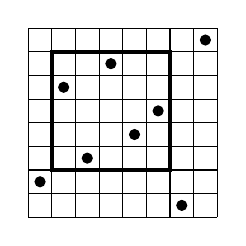
\begin{tikzpicture}[scale=.3]
\draw[thin] (0,0) grid (8,8);
\draw[fill] (.5,1.5) circle (6pt);
\draw[fill] (1.5,5.5) circle (6pt);
\draw[fill] (2.5,2.5) circle (6pt);
\draw[fill] (3.5,6.5) circle (6pt);
\draw[fill] (4.5,3.5) circle (6pt);
\draw[fill] (5.5,4.5) circle (6pt);
\draw[fill] (6.5,0.5) circle (6pt);
\draw[fill] (7.5,7.5) circle (6pt);
\draw [very thick] (1,2) rectangle +(5,5);
\end{tikzpicture}
\caption{Diagram of  and the inflation of  in  by 
\label{fig:graphicalRepresentation}}
\end{center}
\end{figure}

We denote inflations by  where  is a permutation of size  and  is inflated by  for all .
When  is the identity  (resp. the decreasing permutation ) we write  (resp. ).

A permutation  is -decomposable (resp. -decomposable) if it can be written

(resp.  ) with .
Otherwise  is -indecomposable (resp. -indecomposable)

A decomposition theorem \cite{AA05} states that any permutation  can be written in a unique way as either:
\begin{itemize}
\item  where  and the  are -indecomposable.
\item  where  and the  are -indecomposable.
\item where  and  is simple.
\end{itemize}

In the next section we study -stack sorting and -stack pushall sorting and show the close correlation between these two models. 
This combinatorial study concludes on some partial characterization of both classes in terms of permutations they contain or permutations in the basis.
The key idea is to use the block-decomposition of permutations given in the above theorem. 

Then in section~\ref{sec:coloring} we prove that -stack pushall sorting can be expressed as a -color problem on the diagram of permutations.
Moreover we characterize diagram of permutations that can be colored. 
This characterization leads to a polynomial algorithm to check whether a permutation is -stack pushall sortable by finding all colorings for its diagram. 

Section~\ref{sec:optimalAlgo} refines the results of section~\ref{sec:coloring} by limiting the number of colorings to test.
This leads to an optimal algorithm computing in quadratic time a linear representation of all pushall sortings of a given permutation,
which thus decides whether a permutation is \pushall.

To conclude, we give in section~\ref{sec:conclusion} some natural continuations of our work.


\section{-stack sorting vs -stack pushall sorting}

In this section we define pushall sorting and point out the close link between -stack sorting and -stack pushall sorting. 
Moreover, for each of these sorting problems we exhibit some recursive necessary and sufficient conditions for a permutation to be sortable depending on the root of its block-decomposition.

In -stack sorting, three different operations are allowed as pictured in Figure~\ref{fig:rholambdamu}. 
Each of this operation can be encoded with a letter (see Figure~\ref{fig:rholambdamu}).
For example, whenever an element is popped from stack  and pushed in stack , we write . 
A sequence of operations is encoded by a word whose length is the number of operations performed.

\begin{figure}[H]
\begin{center}
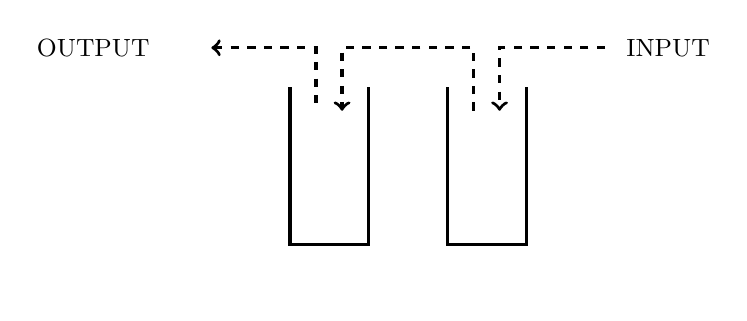
\begin{tikzpicture}
\draw[very thick] (0,2) -- (0,0) -- (1,0) -- (1,2);
\draw (2.5,-0.5) node {};
\draw[very thick] (2,2) -- (2,0) -- (3,0) -- (3,2);
\draw (0.5,-0.5) node {};
\draw[very thick, dashed, ->] (4,2.5) -- node[above] {} (2.66,2.5) -- (2.66,1.7);
\draw (4.8,2.5) node {{\small INPUT}};
\draw[very thick,dashed, ->] (2.33,1.7) -- (2.33,2.5) -- node[above] {} (0.66,2.5) -- (0.66,1.7);
\draw[very thick, dashed, <-] (-1,2.5) -- node[above] {} (0.33,2.5) -- (0.33,1.7);
\draw (-2.5,2.5) node {{\small OUTPUT}};
\end{tikzpicture}
\caption{Sorting with two stacks in series \label{fig:rholambdamu}}
\end{center}
\end{figure}

\begin{defn}
A {\em stack word}  is a word over the alphabet  such that  and for all prefix  of , . 
Intuitively it's a word which describes a sequence of appropriate stack operations which take a permutation through two stacks in series (without necessarily sorting it).
A permutation  is -stack sortable if and only if there exists a stack word of length  ( times each letter ) which leads to the identity in the output with  as input. 
Such a word is called a {\em valid} stack word for .
\end{defn}

There are several valid stack word for a given permutation: for example, permutation  admits either  or  as valid words.
Note also that  and  commutes: if  is a valid stack word for  an  is obtained for  by exchanging adjacent letters  and , then  is a valid stack word for . 
In his Phd \cite{Murphy02}, Murphy studied -stack sorting by studying stack words. 
This presentation of -stack sorting allow us to define formally -stack pushall sorting.

\begin{defn}
A {\em pushall} stack word is a stack word such that the first occurrence of letter  is after the last occurence of the letter .
A permutation  of size  is -stack pushall sortable if and only it admits a valid pushall stack word.

More informally, -stack pushall sortable permutations are those which can be sorted by pushing all elements in the stacks before writing any element to the output.
\end{defn}

For example  is -stack pushall sortable as the word  respects the required condition (as does ). 

\begin{rem}\label{rem:decompoNonUnique}
A stack word  is a pushall stack word if and only if it can be written as  with  and . This decomposition is not unique.
In the preceding example, the word  admits two decompositions:  and .
\end{rem}


The previous definition of -stack pushall sortable permutations implies that they form a subset of -stack sortable permutations. 
Moreover it is easy to check that -stack pushall sorting is stable by pattern relation: if  is -stack pushall sortable then every pattern  of  is -stack pushall sortable: choose an occurrence of  in  and a valid pushall stack word  of . 
To obtain a valid pushall stack word of , delete letters of  that correspond to elements of  not involved in the occurrence of . 
The same reasoning holds for general -stack sorting.

\begin{prop}
-stack pushall permutations form a subclass of -stack sortable permutation class.
\end{prop}


Although we do not know the ratio between these two classes, there exists a close correlation between them and solving -stack pushall sorting is a prerequisite for the more general case. 
We first study the possible configurations of the stacks during a sorting procedure. 
This will help us to obtain properties of stack sorting permutations thanks to their decomposition. 
In a last subsection, we study the basis of -stack sortable permutation class and show how it is correlated to the -stack pushall one.

\subsection{Stack configurations}

At each step of a sorting procedure, some elements of the permutation lie in the stacks. 
We call a {\em stack configuration} the position of these elements in stacks  and . 
In this section, we exhibit a necessary condition on stack configurations to be part of a sorting procedure.
First we define formally stack configurations.

\begin{defn}
A {\em stack configuration} is a pair of two vectors of positive integers  of arbitrairy (and maybe different) sizes, such that all coordinates are distincts.
A stack configuration may be empty (if both vectors are of size zero).
Vector  (resp. ) represents elements that are in stack  (resp. ) given from bottom to top, so we can apply to stack configurations moves  and , and move  if we know what is the next integer in the input.

Let  be a permutation, a stack configuration of  is a stack configuration in which coordinates are bounded by .
\end{defn}


\begin{defn}
To each stack word  of size  and permutation  of size  we associate a sequence of  stack configurations  describing how the sequence of moves  take  through the stacks:  is empty and we obtain  from  by doing operation  with  as input at the beginning.
\end{defn}


\begin{defn}
Let  be a permutation.
A stack configuration  is {\em reachable} for  if it exists a stack word  and an integer  such that .
A stack configuration  is {\em total} for  if all integers from  to  appear in  (this notion depends only on , we don't ask  to be reachable for ).
\end{defn}


\begin{rem}\label{rem:TotalConfigurations}
Let  be a stack word of size  and  a permutation of size .
Then  is a pushall stack word if and only if at least one of the stack configurations  is total.
\end{rem}


During a sorting procedure, stack configurations have constraints so that all elements can be popped out in increasing order. 
Recall that in one-stack sorting, the stack must be in decreasing order (from bottom to top). 
For two-stack sorting, we have the same decreasing constraint on stack  but other constraints appear that can be represented as stack patterns.

\begin{defn}\label{def:unsortableStackPatterns}
We call {\em unsortable stack-patterns} the following three patterns, denoted respectively \patternV, \patternH and \patternVH:
\begin{center}
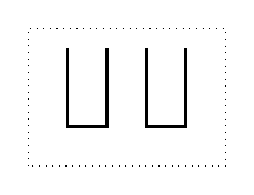
\begin{tikzpicture}[scale=.5]
\draw [dotted] (-1,-1) rectangle +(5,3.5);
\draw[very thick] (0,2) -- (0,0) -- (1,0) -- (1,2);
\draw (2.5,-0.5) node {};
\draw[very thick] (2,2) -- (2,0) -- (3,0) -- (3,2);
\draw (0.5,-0.5) node {};
\draw (0.5,0.5) node {};
\draw (0.5,1.2) node {};
\end{tikzpicture}
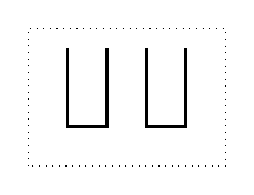
\begin{tikzpicture}[scale=.5]
\draw [dotted] (-1,-1) rectangle +(5,3.5);
\draw[very thick] (0,2) -- (0,0) -- (1,0) -- (1,2);
\draw (2.5,-0.5) node {};
\draw[very thick] (2,2) -- (2,0) -- (3,0) -- (3,2);
\draw (0.5,-0.5) node {};
\draw (2.5,0.5) node {};
\draw (2.5,1.2) node {};
\draw (2.5,1.9) node {};
\end{tikzpicture}
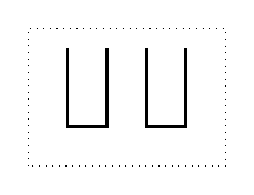
\begin{tikzpicture}[scale=.5]
\draw [dotted] (-1,-1) rectangle +(5,3.5);
\draw[very thick] (0,2) -- (0,0) -- (1,0) -- (1,2);
\draw (2.5,-0.5) node {};
\draw[very thick] (2,2) -- (2,0) -- (3,0) -- (3,2);
\draw (0.5,-0.5) node {};
\draw (2.5,0.5) node {};
\draw (2.5,1.2) node {};
\draw (0.5,0.5) node {};
\end{tikzpicture}
\end{center}
More precisely pattern \patternV means that there is in stack  one element which has a smaller element below it. 
Pattern \patternH means that there is in stack  one element which has a greater element below it and a smaller element more below. 
Pattern \patternVH is somehow special as the pattern is divided in both stacks. 
It means that there are elements  such that , ,  and  is above  in stack . 
\end{defn}



\begin{thm}\label{thm:popable}
A stack configuration can be popped out in increasing order if and only if it avoids each unsortable stack-pattern.
\end{thm}

\begin{proof}
Notice that if a stack configuration contains any of the  unsortable stack-patterns, then elements involved in the pattern cannot be popped out in increasing order.

For the converse, we prove by induction on the number of elements in the stacks that a configuration which avoids the  unsortable stack-patterns can be popped out in increasing order. 
Suppose that the result has been proved for all stack configurations with at most  elements. 
Note that the result is trivially true for . 
Let  be a stack configuration with  elements avoiding the  unsortable stack-patterns and  the smallest element of this configuration.
We show that  can be popped out so that the stack configuration of the  remaining elements still avoids the  unsortable stack-patterns.
Without loss of generality assume .

Suppose that  lies in stack . 
As  avoids pattern \patternV,  is in decreasing order so  is at the top of it. 
It can be popped out and there remains  elements still avoiding the  unsortable stack-patterns. 
Thus they can be all popped out in increasing order by induction. 

Suppose now that  lies in stack . 
As  avoids pattern \patternH and  is the smallest element, all elements above  are in increasing order (from  to top). 
All these elements can be pushed onto stack  so that stack  remains in decreasing order. 
Indeed as  avoids pattern \patternVH , the top of stack  is greater than the top of stack . 
When all elements greater than  and above  in stack  are transferred onto stack , then  can be popped out both stacks  and  and the remaining configuration still avoids the  unsortable stack-patterns (as  avoids pattern \patternH , no pattern \patternVH has been created) and we can apply the induction.
\end{proof}


\begin{rem}\label{rem:uniquePopOut}
There is at most one way to pop out in increasing order elements from a stack configuration. 
Indeed to pop out we only use moves  and , and if we want to pop out in increasing order we have to perform move  if and only if the smallest element lies in the top of .
\end{rem}

\begin{algorithm}[H]
  \SetAlgoLined
\LinesNumbered
  \KwData{ a permutation and  a total stack configuration of .}
  \KwResult{True if  can be popped out in increasing order.}
\;
\While{}{
\eIf{}{
pop out  from stack  and let  
}{
\eIf{ is non empty and }{
pop  from stack  and push it into \;}{
Return false\;
}
}}
Return true\;
 \caption{Pop out in increasing order\label{algo:popOut}}
\end{algorithm}



\begin{prop}\label{prop:AlgoPopOut}
Let  be a total stack configuration of a permutation .
Then Algorithm~\ref{algo:popOut} applied to  returns  \ssi  can be popped out in increasing order.
Moreover Algorithm~\ref{algo:popOut} runs in linear time w.r.t. .
\end{prop}

\begin{pf}
At each step, Algorithm~\ref{algo:popOut} performs either a move  or a move . 
As at most  moves  and  moves  can be done, it runs in linear time w.r.t. .
We conclude using Remark~\ref{rem:uniquePopOut}.
\end{pf}


Theorem~\ref{thm:popable} ensures that a stack configuration can be popped out in increasing order. 
Conditions of this theorem must be verified at each step of a sorting procedure. 
This is formalised in the following proposition:

\begin{prop}\label{prop:eachConfigAvoidUnsortablePattern}
If  is a valid stack word for the permutation , 
then each stack configuration of  avoids the  unsortable stack-patterns.
\end{prop}

The converse is not true: let  then for all permutation  of size  
each stack configuration of  avoids the  unsortable stack-patterns (as it has at most one element in the stacks).
But if  is not the identity,  is not a valid stack word for .

For -stack pushall sorting, however, it is sufficient to check whether the stack configuration obtained 
just after the last element of  has been pushed onto  avoids the  unsortable stack-patterns.

\begin{prop}\label{prop:pushallIffConfigurationEvitePatterns}
A permutation  is \pushall if and only if there is a way to put all its elements in the stacks 
so that the total stack configuration obtained avoids the three unsortable patterns.
\end{prop}

\begin{pf}
If  is \pushall we conclude using Proposition~\ref{prop:eachConfigAvoidUnsortablePattern} and Remark~\ref{rem:TotalConfigurations}. 
The converse is a consequence of Theorem~\ref{thm:popable}.
\end{pf}



\subsection{Decomposition and stack sorting}

In this part we exhibit conditions for a permutation  to be -stack sorted depending on its decomposition. 

\paragraph{-decomposable permutations}: 
\begin{prop}\label{prop:2stacksMoinsDecomposable}
A permutation  is -stack sortable if and only if every  for  is -stack pushall sortable and  is -stack sortable.
\end{prop}
\begin{proof}
Suppose that  is -stack sortable. Let  be a valid stack word of .
For , consider the subword  of  by taking letters corresponding to an element of . 
This word is of size  and has equal number of occurrences of the letters . 
Moreover, it is a valid stack word for  as the relative order of elements of  under the action of  will be the same as the action of  on . 
Furthermore, as the element  in  belongs to the last block , all elements of  are pushed into the stacks before the first pop. 
Hence  is -stack pushall sortable. 
-stack sortable permutations form a permutation class, so that  must be -stack sortable.

Conversely, if every  for  is -stack pushall sortable and  is -stack sortable, let  () be a pushall stack word for  and  be a stack word for . 
Then each  () can be written as  where  contains no occurrence of  and  no occurrence of .
It is easy to check that the word  is a valid stack word for , hence  is -stack sortable.
\end{proof}

With a similar proof, we have the following result when restricting to \pushall permutations:

\begin{prop}\label{prop:pushallMoinsDecomposable}
A permutation  is \pushall if and only if every  for  is -stack pushall sortable.
\end{prop}

\paragraph{-decomposable permutations}

The case where  is -decomposable is a bit different as each block of the decomposition can be popped out as soon as they are pushed into the stacks. 
So the only condition is given in the following proposition.

\begin{prop}
If  then  is -stack sortable if and only if each  is -stack sortable.
\end{prop}

For \pushall permutations, -decomposable permutations are harder to handle. 
As no element can be popped out before all elements have been pushed, the element  which belongs to the first block must remain in the stacks until every element is pushed. 
This induces several constraints which are proved in the following propositions. 
All these propositions aim at proving Theorem~\ref{thm:+pt} which fully characterizes -decomposable \pushall permutations.

\begin{thm}
\label{thm:+pt}
Let  be a -decomposable permutation. Then  is \pushall if and only if  avoids

\end{thm}

The proof proceeds step by step in Propositions~\ref{CS} to \ref{prop:+[1,x,1]pt}.

\begin{prop}\label{CS}
Let  be a permutation such that either:
\begin{itemize}
\item 
\item 
\item 
\item 
\end{itemize}
Then  is \pushall.
\end{prop}
\begin{proof}
We show that we can put all elements of  in the stacks so that they avoid patterns of Theorem~\ref{thm:popable} (p.\pageref{thm:popable}).
In the first case, just push every element in stack . 
For the second case, we know from Knuth \cite{Knuth73} that each permutation avoiding  can be sort in increasing order with one stack. 
So each permutation avoiding  can be sort in deacreasing order with one stack. 
Hence we can use stack  to push all elements of  in decreasing order onto stack . 
For the last two cases, we push the elements in corresponding stacks  for  and  for . 
In each case, the stack configuration respect conditions of Theorem~\ref{thm:popable}.
\end{proof}

Note that Proposition~\ref{CS} give a sufficient condition which is not necessary: the permutation  is \pushall but do not belong to one of the preceding cases. 
In this proposition, an important role is given to classes  and . 
These indeed are exactly the classes of permutations that can be pushall sorted with a stack configuration where all elements lie in one {\em single} stack ( for  and  for ). 
Thus the only difficult case is whenever a permutation contains both pattern  and . 
This is characterized by the following proposition:

\begin{prop}\label{prop:132et213}
A permutation  contains both patterns  and  if and only if it contains one of the following patterns:
 and .

\begin{figure}[H]
\begin{center}
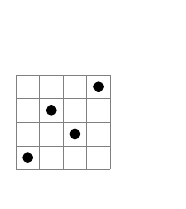
\begin{tikzpicture}[scale=.30]
\useasboundingbox (1.5,0.5) rectangle (7,7);
\permutation{1,3,2,4}
\end{tikzpicture}
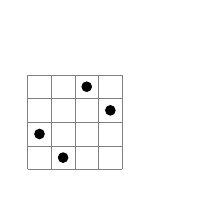
\begin{tikzpicture}[scale=.30]
\useasboundingbox (1,0.5) rectangle (7,7);
\permutation{2,1,4,3}
\end{tikzpicture}
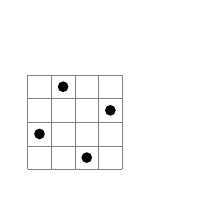
\begin{tikzpicture}[scale=.30]
\useasboundingbox (1,0.5) rectangle (7,7);
\permutation{2,4,1,3}
\end{tikzpicture}
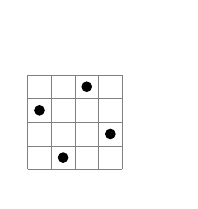
\begin{tikzpicture}[scale=.30]
\useasboundingbox (1,0.5) rectangle (7,7);
\permutation{3,1,4,2}
\end{tikzpicture}
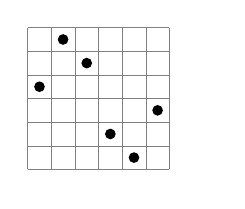
\begin{tikzpicture}[scale=.30]
\useasboundingbox (1,0.5) rectangle (9,7);
\permutation{4,6,5,2,1,3}
\end{tikzpicture}
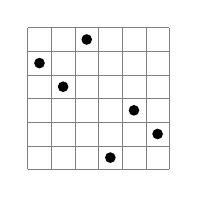
\begin{tikzpicture}[scale=.30]
\useasboundingbox (1,0.5) rectangle (8,7);
\permutation{5,4,6,1,3,2}
\end{tikzpicture}
\caption{Minimal permutations containing patterns  and .}
\label{fig:132et213}
\end{center}
\end{figure}
\end{prop}

\begin{proof}
Minimal permutations that contain both  and  are exactly permutations of the basis of . 
By minimality of the elements of the basis those permutations are at most of size  and a comprehensive study ends the proof.
\end{proof}

To prove a complete characterization of -decomposable \pushall permutations, we deal first with permutations whose decomposition contains non-trivial block -i.e. blocks not reduced to a singleton-.

\begin{prop}
\label{prop:B1}
Suppose  with , each  -indecomposable and blocks  and  are non-trivial. 
Then  is \pushall if and only if  avoids every pattern of .
\end{prop}
\begin{proof}



We state by checking each pushall stack word of the right size that permutations of  are not \pushall. 
Hence if  is \pushall it avoids . 
Conversely, let  be a permutation avoiding every pattern of . 
As  and  are non-trivial and -indecomposable, they contain  as a pattern. 
But  avoids  so that blocks  with  are trivial. 
Let  contains pattern  and  contains pattern . 
These sets are included in  and not equal to  as  avoids  and .
\begin{itemize}
\item If , then  and  so  and  is \pushall by Proposition~\ref{CS}.
\item If  and , then .
If  then  and  hence  and  is \pushall by Proposition~\ref{CS}.
If , as  avoids  then , but  and  hence . 
So  is \pushall by Proposition~\ref{CS}.

\item If  and , then .
If , as  avoids  then , but  and  hence . 
So  is \pushall by Proposition~\ref{CS}.
If  then  and  hence  and  is \pushall by Proposition~\ref{CS}.

\item If .
If  then  and  as  avoids . 
But  and  hence  and  is \pushall by Proposition~\ref{CS}.
If  then ,  and  hence . 
So  is \pushall by Proposition~\ref{CS}.

\item If , then by Proposition~\ref{prop:132et213},  contains either ,  or . 
We prove that  contains a pattern of . 
If  contains , either , and  would contain  or , and  would contain . 
Similarly if  contains ,  would contain . 
The same goes for  containing , ,  or . 
Hence the case  cannot occur.
\end{itemize}
\end{proof}


Given two permutation classes  and , their horizontal juxtaposition   consists of all permutations  that can be written as a concatenation  
where  is order isomorphic to a permutation in  and  is order-isomorphic to a permutation in . 
In other words, a diagram of a permutation  can be divided by  a vertical line into two parts, 
such that the left one is order-isomorphic to a permutation of  and the right one to a permutation of . 
We can similarly define the vertical juxtaposition   consisting of permutations having a diagram cut by a horizontal line.

\begin{prop}
\label{prop:+[1,x]pt}
A permutation  is \pushall if and only if \\
 and there exists an associated decomposition  
such that there are no pattern  in  where  is in  and  is in .
\end{prop}
\begin{proof}
If  with this decomposition satisfying hypothesis of the proposition, then  is \pushall using the following algorithm. 
Put  in . 
Then push elements of  in stack  in decreasing order. 
Then put  at top of  and finally push every element of  onto . 
As there are no pattern  in  with  in  and  in , the stack configuration respects conditions of Theorem~\ref{thm:popable} hence can be popped out.

Conversely, suppose that  is \pushall and consider a stack word for this permutation. 
As  is the first element, it is pushed at the bottom of . 
Then some elements are pushed onto  and into  before  is popped out from stack  to stack . 
The remaining elements are pushed into  as they are greater than . 
We consider the moment where all elements have been pushed and  is at the top of . 
This separates in two parts the elements of  taking  as the elements in  and  the elements in  apart from . 
From Theorem~\ref{thm:popable} decomposition  satisfies conditions of the statement.
\end{proof}

\begin{prop}
\label{prop:B2}
Let  is \pushall . 
Then  is a finitely based permutation class whose basis is .
\end{prop}

\begin{proof}
As \pushall permutations is a permutation class, so does . 
Let  be the basis of . 
To prove that  is finite, we first prove that every permutation in  has size less than . 
Then an comprehensive computation gives the permutations in .

By Proposition~\ref{prop:+[1,x]pt},  and there are no pattern  in  where  is in  and  is in . 
Let . 
By definition  so  and . 
Let  be a pattern  such that  is maximal and  be a pattern  such that  is minimal, then  minimal (for  fixed) and finally  maximal (for  and  fixed).
\begin{itemize}
\item If  then , hence by minimality of the basis  so .
\item If  then  and by minimality  so .
\item If , consider the pattern  (shown in Figure~\ref{fig1Preuve}). 
Minimality conditions for  and  and maximality condition for  imply that gray zones in the diagram of  are empty. 
So . 
As , there is no possible cut  such that ,  and there are no pattern  in  where  is in  and  is in . 
Hence, all cuts in  are forbidden, either because they are to the left of a  pattern or to the right of a  pattern or between element  and  of a pattern . 
More specially the cut between  and  is forbidden. 
This cut cannot be to the left of a pattern  by maximality of  () and cannot be to the right of a pattern  by minimality of . 
So this cut is between elements  and  of a pattern . 
We consider a pattern  denoted by  such that  is minimal and  is minimal for  fixed among patterns  such that  and .

\begin{figure}[H]
\begin{minipage}[b]{.22\linewidth}
\begin{center}
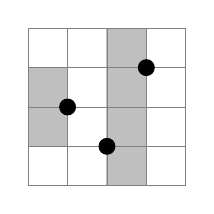
\begin{tikzpicture}[scale=.5]
\draw [fill, lightgray] (2,0) rectangle (3,4);
\draw [fill, lightgray] (0,1) rectangle (1,3);
\draw [help lines] (0,0) grid (4,4);
\draw (2,1) [fill] circle (0.2);
\node at (2.5,0.6) {{\scriptsize}};
\draw (3,3) [fill] circle (0.2);
\node at (3.5,3.4) {{\scriptsize}};
\draw (1,2) [fill] circle (0.2);
\node at (0.6,2.4) {{\scriptsize}};
\end{tikzpicture}
\caption{}
\label{fig1Preuve}
\end{center}
\end{minipage}
\begin{minipage}[b]{.23\linewidth}
\begin{center}
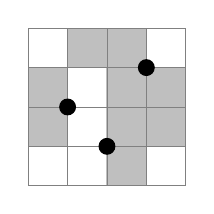
\begin{tikzpicture}[scale=.5]
\draw [fill, lightgray] (2,0) rectangle (3,4);
\draw [fill, lightgray] (0,1) rectangle (1,3);
\draw [fill, lightgray] (1,3) rectangle (2,4);
\draw [fill, lightgray] (3,1) rectangle (4,3);
\draw [help lines] (0,0) grid (4,4);
\draw (2,1) [fill] circle (0.2);
\node at (2.5,0.6) {{\scriptsize}};
\draw (3,3) [fill] circle (0.2);
\node at (3.5,2.6) {{\scriptsize}};
\draw (1,2) [fill] circle (0.2);
\node at (0.6,2.4) {{\scriptsize}};
\node at (3.5,3.5) {{\small}};
\node at (3.5,0.5) {{\small}};
\node at (0.5,3.5) {{\small}};
\node at (0.5,0.5) {{\small}};
\end{tikzpicture}
\caption{Cas }
 \label{fig2Preuve}
\end{center}
\end{minipage}
\begin{minipage}[b]{.25\linewidth}
\begin{center}
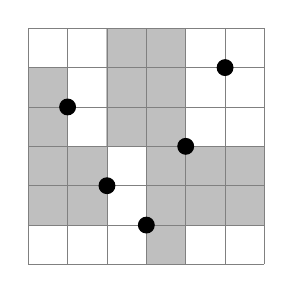
\begin{tikzpicture}[scale=.5]
\draw [fill, lightgray] (2,3) rectangle (4,6);
\draw [fill, lightgray] (0,1) rectangle (1,5);
\draw [fill, lightgray] (1,1) rectangle (2,3);
\draw [fill, lightgray] (3,1) rectangle (6,3);
\draw [fill, lightgray] (3,0) rectangle (4,1);
\draw [help lines] (0,0) grid (6,6);
\draw (3,1) [fill] circle (0.2);
\node at (3.5,0.6) {{\scriptsize}};
\draw (4,3) [fill] circle (0.2);
\node at (4.5,3.4) {{\scriptsize}};
\draw (2,2) [fill] circle (0.2);
\node at (1.6,2.4) {{\scriptsize}};
\draw (1,4) [fill] circle (0.2);
\node at (0.6,4.4) {{\scriptsize}};
\draw (5,5) [fill] circle (0.2);
\node at (5.5,5.4) {{\scriptsize}};
\node at (0.5,5.5) {{\small}};
\node at (0.5,0.5) {{\small}};
\end{tikzpicture}
\caption{}
 \label{fig3Preuve}
\end{center}
\end{minipage}
\begin{minipage}[b]{.25\linewidth}
\begin{center}
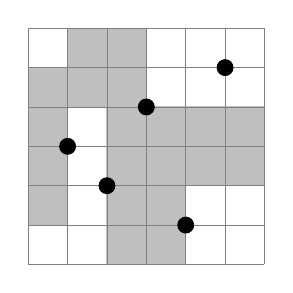
\begin{tikzpicture}[scale=.5]
\draw [fill, lightgray] (2,0) rectangle (4,2);
\draw [fill, lightgray] (0,1) rectangle (1,5);
\draw [fill, lightgray] (1,4) rectangle (3,6);
\draw [fill, lightgray] (2,2) rectangle (6,4);
\draw [help lines] (0,0) grid (6,6);
\draw (2,2) [fill] circle (0.2);
\node at (2.5,1.6) {{\scriptsize}};
\draw (3,4) [fill] circle (0.2);
\node at (3.5,4.4) {{\scriptsize}};
\draw (1,3) [fill] circle (0.2);
\node at (0.6,3.4) {{\scriptsize}};
\draw (4,1) [fill] circle (0.2);
\node at (4.5,0.6) {{\scriptsize}};
\draw (5,5) [fill] circle (0.2);
\node at (5.5,5.4) {{\scriptsize}};
\node at (0.5,5.5) {{\small}};
\node at (0.5,0.5) {{\small}};
\end{tikzpicture}
\caption{}
 \label{fig4Preuve}
\end{center}
\end{minipage}
\end{figure}

\begin{itemize}
\item If  then . 
Indeed all cuts are forbidden: 
those before  by , between  and  by , between  and  by  and before  by . 
So by minimality of the basis .
\item If , we want to prove that . 
Then  since all cuts are forbidden as before and .
As  and  maximal, gray zones added in Figure~\ref{fig2Preuve} are empty. 
As ,  and  lie either both in , or both in , or  lies in  and  in .
\begin{itemize}
\item If  and  lie both in , then  lies in  and  form the permutation  and as  is maximal, .
\item If  and  lie both in , then  lies in  and by minimality of  we have . 
 is minimal, so that gray zones added in Figure~\ref{fig3Preuve} are empty. 
Suppose that . 
The cut between  and  is forbidden as . 
As  is maximal the cut cannot be to the left of a pattern , neither to the right of a pattern  by minimality of . 
Hence the cut lies between element  and  of a pattern . 
Let  be such a pattern  such that  and . 
Then  and  lies in area  or  and  by minimality of . 
If  lies in  then  is the pattern , which is forbidden by minimality of . 
Hence  lies in  and  otherwise  is a pattern  with , which is also forbidden by minimality of . 
Hence  is a pattern  with  and  which is impossible by minimality of .
\item If  lies in  and  in , by minimality of ,  or  lies in  or  lies in . 
If  lies in  then  is a pattern  which contradicts the minimality of . 
If  lies in ,  is a pattern  hence . 
If , by minimality of  then , gray zones added in Figure~\ref{fig4Preuve} are empty. 
The cut between  and  is forbidden as . 
As before the cut lies between elements  and  of a pattern . 
Let  such a pattern  such that  and . 
Then  and  lies in  or  and  by minimality of . 
If  lies in  then  is a pattern  and by minimality of , . 
If  lies in  then  otherwise  is a pattern  with , which is forbidden by maximality of . 
But  is a pattern  with  and , so by minimality of , .
\end{itemize}
\end{itemize}
\end{itemize}

\end{proof}


\begin{prop}
\label{prop:+[x,1]pt}
A permutation  is \pushall if and only if  and there exists an associated decomposition  such that there is no pattern  in  where element  is in  and elements  and  are in .
\end{prop}

\begin{proof}
Let . 
Consider a pushall sorting of . 
This permutation has  as last element, so that we consider the configuration of the stacks just after the insertion of . 
By Theorem~\ref{thm:popable}, it must avoid the pattern \patternVH, so that all elements in  -under - are greater than those of .
Hence we can write  where  contains elements of  and  those in  -except -.
Then from Theorem~\ref{thm:popable}  and  and that there are no pattern  in  where element  is in  and elements  and  are in .

Conversely, suppose that there exists a decomposition  respecting the previous conditions then we have a pushall sorting of the permutation  using the following algorithm.
While the input is not empty, if stack  is empty or if the top of  belongs to , we push the next element of the input onto . 
If , the top of  belongs to , and if the next element of the input  belongs to  and is greater than , we push  onto , otherwise we pop  from  and push it onto . 
At each step we verify conditions of Theorem~\ref{thm:popable} so that all elements can be popped out in increasing order at the end.
\end{proof}


\begin{prop}
\label{prop:B3}
Let  is \pushall . 
 is a finitely based permutation class whose basis is .
\end{prop}
\begin{proof}
As the set of \pushall permutations is a permutation class, so is . 
By Proposition~\ref{prop:+[x,1]pt},  such that there exists an associated decomposition  such that there is no pattern  in  where element  is in  and elements  and  are in \}.
Hence  and  are in one-to-one correspondence by taking an element of , rotate its diagram by  and apply the symmetry with respect to axis . 
If elements are in one-to-one correspondence by rotation and symmetry so does the basis which proves the result.
\end{proof}


\begin{prop}
\label{prop:+[1,x,1]pt}
A permutation  is \pushall if and only if .
\end{prop}
\begin{proof}
By Proposition~\ref{prop:+[1,x]pt},  is \pushall if and only if  and there exists a corresponding decomposition  such that there is no pattern  in  where element  is in  and  are in , which is equivalent to  and there exists a corresponding decomposition  such that there are no pattern  in  where element  is in  and element  is in , i.e. .
\end{proof}

We are now able to prove Theorem~\ref{thm:+pt} (p.\pageref{thm:+pt}).

\begin{proof}
Permutations of  are not \pushall (check each pushall stack word of the right size), hence if  is \pushall it avoids . 
Conversely suppose that  avoids . 
Let  be the -decomposition of  with  and  -indecomposable for all .
\begin{itemize}
\item If  and  are non trivial then  is \pushall thanks to Proposition~\ref{prop:B1}. 
Indeed  avoids  as .
\item If  is trivial then  and  avoids  so that  is \pushall by Proposition~\ref{prop:B2}.
\item If  is trivial then  and  avoids  hence  is \pushall by Proposition~\ref{prop:B3}.
\end{itemize}
\end{proof}



We call {\em separable} permutations the class .

\begin{thm}
Let  be a separable permutation. 
 is \pushall if and only if  avoids .
\end{thm}
\begin{proof}
As permutations of  are not \pushall, every \pushall permutation avoids . 
Conversely, supppose that  avoids . 
As  is separable,  is either -decomposable or -decomposable or trivial (i.e. of size 1), and  avoids  and  which added to constraints of  gives that  avoids , the set defined in Theorem~\ref{thm:+pt}.
If  is -decomposable, then  is \pushall by Theorem~\ref{thm:+pt}.
If  is -decomposable, then  where each  is either trivial or -decomposable. 
So  is \pushall by Proposition~\ref{prop:pushallMoinsDecomposable} and Theorem~\ref{thm:+pt}.
\end{proof}





\subsection{Basis of stack sorting class}
In the previous section, we show that \pushall separable permutations form a finitely based permutation class. 
This property does not hold for \pushall permutations and we exhibit an infinite antichain in the following proposition.

\begin{prop}
The basis of \pushall permutation is infinite.
\end{prop}

\begin{proof}
Consider permutations  for .
The first ones are depicted in Figure~\ref{fig:antichaine}. These permutations are simple and incomparable.
To complete the proof, straightforward though technical, just check that those permutations are not \pushall and that every pattern 
of these permutations are \pushall.

\begin{figure}[ht]
\begin{center}
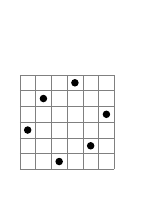
\begin{tikzpicture}[scale=.2]
\useasboundingbox (1.5,0.5) rectangle (8,10);
\permutation{3,5,1,6,2,4}
\end{tikzpicture}
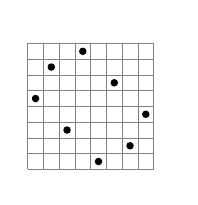
\begin{tikzpicture}[scale=.2]
\useasboundingbox (1,0.5) rectangle (10,10);
\permutation{5,7,3,8,1,6,2,4}
\end{tikzpicture}
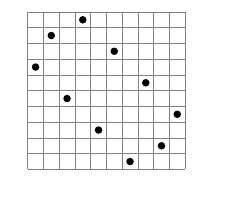
\begin{tikzpicture}[scale=.2]
\useasboundingbox (1,0.5) rectangle (12,10);
\permutation{7,9,5,10,3,8,1,6,2,4}
\end{tikzpicture}
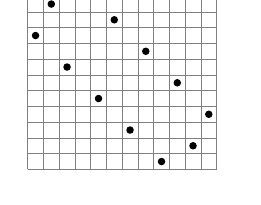
\begin{tikzpicture}[scale=.2]
\useasboundingbox (1,0.5) rectangle (14,10);
\permutation{9,11,7,12,5,10,3,8,1,6,2,4}
\end{tikzpicture}
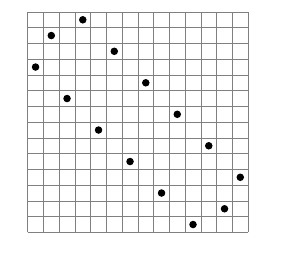
\begin{tikzpicture}[scale=.2]
\useasboundingbox (1,0.5) rectangle (16,14);
\permutation{11,13,9,14,7,12,5,10,3,8,1,6,2,4}
\end{tikzpicture}
\caption{An antichain of the basis of \pushall permutations class.}
\label{fig:antichaine}
\end{center}
\end{figure}

\end{proof}

Note that the basis is infinite and contains a infinite number of simple permutations, and the \pushall class contains also an infinite number of simple permutations.

\begin{prop}\label{prop:basePushallTriable}
If  is in the basis of \pushall permutations, then  is -stack sortable.
\end{prop}
\begin{proof}
Let  be in the basis of \pushall permutations. 
By definition,  is \pushall. 
We can sort  (not pushall sort ) using the following algorithm. 
Push all elements  to  in the stacks following the \pushall operations of . 
Then pop elements , then push  and pop it to the output and pop the remaining elements. 
It is easy to check that these operations are allowed.
\end{proof}

Those last two propositions give a partial characterization of the basis of \pushall permutations class and -stack sortable permutations. 
A more accurate result can be given for certain type of permutations in the basis.


\begin{prop}
Let  be a -decomposable permutation. 
Then  belongs to the basis of -stack sortable permutations class if and only if  where  belongs to the basis of \pushall permutations class.
\end{prop}

\begin{proof}
Let  with  a pemrutation of the basis of \pushall permutations class. 
Proposition~\ref{prop:2stacksMoinsDecomposable} ensures that  is not -stack sortable. 
Note also that every pattern of  is -stack sortable. 
To prove this result, suppose that you remove a point in the permutation. 
Suppose we delete element  then the obtained permutation is , hence it is -stack sortable by Proposition~\ref{prop:basePushallTriable}. 
Otherwise we delete an element of  leading to  which is \pushall by the definition of a permutation class basis. 
Then,  is -stack pushall sortable using Proposition~\ref{prop:2stacksMoinsDecomposable}. 

Conversely, if  belongs to the basis of -stack sortable permutations class, then by Proposition~\ref{prop:2stacksMoinsDecomposable}, either  is not -stack sortable which contradicts the minimality of  ( is an element of the basis so that every pattern of  must belong to the class) or there exists  such that  is not \pushall. 
But in that case,  is not -stack sortable by Proposition~\ref{prop:2stacksMoinsDecomposable} hence  by minimality of basis elements. 
If  has a proper pattern  which is not \pushall then  is a proper pattern of  which is not -stack sortable. 
This is impossible as  belongs to the basis of -stack sortable permutations class. 
So  belongs to the basis of \pushall permutations class, which concludes the proof.
\end{proof}

\section{Sorting and bi-coloring}\label{sec:coloring}

\subsection{A simple characterization}
There is a natural relation between -stack pushall sorting and coloring of permutation diagram into two colors. 
The key idea is to look at the stack configuration once all elements of the permutation are pushed into the stacks. 
Then each element of the permutation belong either to stack  or to stack .
We assign a color to them depending in which stack they lie at this particular step of the sorting. 
In this article we color like \Hzone points that lie in stack  and like \Vzone points in stack .

However by Remark \ref{rem:decompoNonUnique}, this stack configuration is not unique, and neither is the coloring.

\begin{defn}\label{def:validColoring}
A {\em bicoloring} of a permutation  is a coloring of the points of the diagram of  with two colors \G and \R.

A {\em valid coloring} is a bicoloring which avoids each of the four following colored pattern:
\begin{itemize}
\item pattern \RRR: there is a pattern  in \R
\item pattern \GGG: there is a pattern  in \G
\item pattern \GGR: there is a point of \R lying vertically between a pattern  of \G
\item pattern \RRG: there is a point of \G lying horizontally between a pattern  of \R
\end{itemize}
\end{defn}


\begin{defn}
Let  be a permutation. 
To each total stack configuration of  the map  assigns the bicoloring of  such that elements of  are in \R and elements of  are in \G.
To every bicoloring of a permutation  the map  associates the total stack configuration of  such that elements of \G lie in  in decreasing order of value from bottom to top and elements of \R lie in  in increasing order of indices from bottom to top.
\end{defn}

\begin{rem}\label{rem:Col/Conf}
For any bicoloring , .
For any stack configuration  such that elements of  are in decreasing order of value from bottom to top and elements of  are in increasing order of indices from bottom to top, .
\end{rem}


\begin{prop}\label{prop:AlgoPush}
Let  be a bicoloring of a permutation .
Then Algorithm~\ref{algo:Push} applied to  returns  \ssi  is reachable for .
In this case the stack configuration to which Algorithm~\ref{algo:Push} leads is .
\end{prop}

\begin{algorithm}
 \SetAlgoLined
\LinesNumbered
  \KwData{ a permutation and  a bicoloring of .}
  \KwResult{True if the stack configuration corresponding to  is reachable from .}
Begin with the empty stack configuration and  as input and \;
\While{}{
  \eIf{ is empty or }{
      push  into \;
      \;
  }( {\it /*  */})
  {
  \eIf{ or }{
      \eIf{ is empty or }{
           pop  from stack  and push it into \;
      }{Return false\;}
  }( {\it /* ,   and */})
  {
  push  into \;
  \;
  }
  }
}
\While{ is nonempty and }{
  \eIf{}{
      pop  from stack  and push it into \;
  }{Return false\;}
}
Return true\;
\caption{Algorithm to obtain a reachable configuration compatible with a bicoloring}
\label{algo:Push}
\end{algorithm}

To state this proposition we need the two following lemmas:

\begin{lem}\label{lem:configAlgoPush}
At each step of Algorithm~\ref{algo:Push}, the stack configuration we have is reachable for , elements of  are in increasing order of indices from bottom to top, elements of  are in decreasing order of value from bottom to top, there is no element of \R in , there is no element of \R above an element of \G in  and elements of \G that lie in  are in increasing order of value from bottom to top.

Moreover index  verifies that if  then  is the next element of the input and if  then there is no more element in the input.
\end{lem}

\begin{pf}
The proof is by induction on the number of stack operations performed by the algorithm.
Algorithm~\ref{algo:Push} begins with the empty stack configuration and  as input and  so the properties are true at the beginning. Algorithm~\ref{algo:Push} performs only appropriate stack operations so at each step the configuration obtained is reachable for .
Moreover in a reachable configuration, elements of  are in increasing order of indices.
When an element is put in  (this happens at line  or ) then this element is in \G (checked at line  or ) and is smaller than the top of  (checked at line  or ) so that elements of  remain in decreasing order of value from bottom to top and  contains no element of \R. 
When we put an element in , it can be at line  or . 
In the first case,  is empty or its top is in \R (checked at line ) so all its elements are in \R by induction hypothesis. 
In the second case, the top of  is in \G and the element we put in  is in \G and greater than the top of . 
This ensures that there is no element of \R above an element of \G in  and that elements of \G that lie in  are in increasing order from bottom to top (using induction hypothesis). 
Finally  is increased exactly when  is put into  so the last property remains true.
\end{pf}


\begin{lem}\label{lem:AlgoPushTerminates}
Algorithm~\ref{algo:Push} terminates in linear time w.r.t .
\end{lem}

\begin{pf}
At each step, Algorithm~\ref{algo:Push} performs either a legal move , or a legal move , or return false or true (and stops). 
As at most  legal moves  and  legal moves  can be done, Algorithm~\ref{algo:Push} terminates after at most  steps. 
As each step is done in constant time, we have the result.
\end{pf}

We are now able to prove Proposition~\ref{prop:AlgoPush}:

\begin{pf}
If Algorithm~\ref{algo:Push} applied to  returns true, then it reaches line . 
In particular the loop of line  stops so the top of  is not in \G. 
Thus by Lemma~\ref{lem:configAlgoPush} there is no element of \G in . 
In addition by the same lemma elements of  are in increasing order of indices from bottom to top, elements of  are in decreasing order of value from bottom to top and there is no element of \R in . 
So the stack configuration we have is .
Moreover Lemma~\ref{lem:configAlgoPush} states that the stack configuration we have is reachable for , so  is reachable for .

Conversely if  is reachable for , then there is a sequence  of appropriate stack operations so that the configuration obtained with  as input is . 
Let us prove that the sequence of moves  performed by Algorithm~\ref{algo:Push} applied to  is . 
We prove by induction on  () that  and  have the same prefix of length  (obvious for ). 
First notice that as  is a total stack configuration, so  has no letter , and that Algorithm~\ref{algo:Push} performs only moves  and , so  has no letter . 
Suppose that  and  have the same prefix  of length  with , let  be the stack configuration obtained after permforming moves of  with  as input. 
We want to prove that  exists and . 
By definition of ,  is the move performed by Algorithm~\ref{algo:Push} in configuration  (setting by extension  if Algorithm~\ref{algo:Push} terminates in configuration , i.e. if ), and by defintion of ,  is a move which allows to go from configuration  to configuration  (maybe with some additional moves).

We check the value of  after Algorithm~\ref{algo:Push} has performed moves . 
We know that at this step stacks are in configuration .

If , then from Lemma~\ref{lem:configAlgoPush} in configuration  all elements of  lie already in the stacks. 
As  is a sequence of appropriate stack operations, then  so  ( has no letter ). 
As  is a move which allows to go from configuration  to configuration  in which there is no elements of \R in  and  is decreasing, then the top of  in  is in \G and smaller than the top of  (or  is empty). 
As  and as the top of  in  is in \G and smaller than the top of  (or  is empty) then Algorithm~\ref{algo:Push} performs line  so .

If  then we are in the loop beginning at line~ of the algorithm and from Lemma~\ref{lem:configAlgoPush}  is the next element of the input. 
Suppose that . 
As  is a legal move which allows to go from configuration  to configuration  in which there is no elements of \R in  and  is decreasing, then  is non empty, the top of  is in \G and smaller than the top of . 
Suppose in addition that . 
As  is still on the input after  and  is a move which allows to go to configuration  in which  is decreasing, then  is smaller than the top of  in . 
So either  or . 
So from  Algorithm~\ref{algo:Push} performs line  so .

Suppose that . 
If in configuration  stack  is empty or top(H)  then Algorithm~\ref{algo:Push} performs line  so . 
Otherwise let  be the top of  in , then . 
So  in . 
But once  is performed  is above  in . 
As  is a move which allows to go from configuration  to configuration  then  is below  in  in  (indeed it is impossible that  goes to stack  and  remains in stack ). 
So  and as in  elements of  are in decreasing order, . 
So the test of line  of the algorithm is false and Algorithm~\ref{algo:Push} performs line  so .

This ends the induction. 
We have proved that  is a prefix of , so Algorithm~\ref{algo:Push} reaches configuration . 
We have now to prove that Algorithm~\ref{algo:Push} stops in this configuration and returns true.

When  is reached then there is no element in the input anymore, so from Lemma~\ref{lem:configAlgoPush} , and  in . 
So both loops while of Algorithm~\ref{algo:Push} are finished and the algorithm reaches line , returns true and terminates in configuration .
\end{pf}

\begin{lem}\label{lem:AlgoFalse}
Let  be a bicoloring of a permutation .
If Algorithm~\ref{algo:Push} applied to  returns  then  has a pattern \GGR or a pattern \GGG.
\end{lem}

\begin{pf}
We consider the stack configuration reached when Algorithm~\ref{algo:Push} returns . 
We set  and . 
By Lemma~\ref{lem:configAlgoPush}, . 
Algorithm~\ref{algo:Push} returns  by reaching either line  or line . 
In both cases,  and . 
Now we consider the step of the algorithm where  was put in , the indice  at this step of the algorithm, and the corresponding configuration  just before the move putting  into  is done. 
So at this step  is on the top of , and . 
If  is in  in , then it is below , contradicting Lemma~\ref{lem:configAlgoPush} ( and both are in \G). 
As  is in  when the algorithm ends, it cannot be in  in . 
So  is still in the input and . 
Recall that we consider the step of the algorithm where  is put in . 
This can happen at line  or  but  so it is at line . 
So the test of line  is true, thus either  and then  is a pattern \GGR of , or  but  and then  is a pattern \GGG of .
\end{pf}



\begin{thm}\label{thm:bijectionColoriageConfiguration}
The map  is a bijection from the set of reachable total stack configuration of  avoiding the three unsortable patterns to the set of valid coloring of .
Moreover the inverse of  is the map .
\end{thm}

\begin{pf}
Let  be a reachable total stack configuration of  avoiding the three unsortable patterns and set . 
We have to prove that  avoids every forbidden colored pattern of Definition~\ref{def:validColoring}.

If  has a pattern  in \R then there are three element ,  and  of \R such that  and . 
By definition of , ,  and  lie in . 
As  is reachable and ,  is below  which is below . 
So we have a stack-pattern \patternH in  which contradicts our hypothesis. 
So  has no pattern \RRR.

If  has a pattern  in \G then there are three element ,  and  of \G such that  and . 
By definition of , ,  and  lie in . 
As  avoids stack-pattern \patternV,  is below  which is below . 
But then  is not reachable: as  is below  and  in ,  and  have to stay in stack  until  enters stack . 
But as ,  is below  in stack  and cannot be below  in stack  as going from stack  to stack  reverse the order. 
So  has no pattern \GGG.


If  has a point of \R lying vertically between a pattern  of \G then there are elements  and  of \G and  of \R such that  and . 
By definition of ,  and  lie in  and  lies in . 
Configuration  is reachable. 
We consider a sequence of stack operations leading to . 
As ,  is already in the stacks when  enters . 
As  remains in  in  but  is in  in ,  has to be already in  when  enters stack . 
As , at this moment  is not already in stack , so  will be above  in  and they form a pattern \patternV in , which is excluded. 
So  has no pattern \GGR.

If  has a point of \G lying horizontally between a pattern  of \R then in  these points form a pattern \patternVH which is excluded. 
So  has no pattern \RRG.


Conversely let  be a valid coloring of .
By definition  is a total stack configuration of .
We have to prove that  is reachable for  and avoids the three unsortable stack patterns.
As  is a valid coloring, it avoids patterns \GGR and \GGG. 
So from Lemma~\ref{lem:AlgoFalse}, Algorithm~\ref{algo:Push} started with input  returns true.
Thus from Proposition~\ref{prop:AlgoPush},  is reachable for . 
Moreover by definition of ,  avoids pattern \patternV. 
Furthermore we know that in , elements of  are in increasing order of indices from bottom to top. 
So if  has a pattern \patternH, then  has a pattern \RRR, and if  has a pattern \patternVH then  has a pattern \RRG. 
A  is a valid coloring, we conclude that  avoids the three unsortable stack patterns.

Now using Remark~\ref{rem:Col/Conf} it's clear that  is the inverse of .
\end{pf}


\begin{thm}\label{thm:equivalenceColoringPushall}
A permutation  is \pushall \ssi its diagram admits a valid coloring.
\end{thm}

\begin{pf}
Consequence of Proposition~\ref{prop:pushallIffConfigurationEvitePatterns} and Theorem~\ref{thm:bijectionColoriageConfiguration}.
\end{pf}

Now thank to Theorem~\ref{thm:equivalenceColoringPushall} we have a naive algorithm to check if a permutation  is \pushall: forall bicoloring  of , we can test if  is valid by checking if  avoids patterns \GGG, \GGR, \RRG and \RRR of Definition~\ref{def:validColoring}.
But first notice that we have a more efficient way to test if a bicoloring is valid:

\begin{prop}\label{prop:Check-Valid-linear}
Let  be a bicoloring of a permutation .
We can check in linear time w.r.t.  if  is a valid coloring.
More precisely,  is a valid coloring \ssi Algorithm~\ref{algo:Push} applied to  returns true and Algorithm~\ref{algo:popOut} applied to  returns true.
\end{prop}

\begin{pf}
From Theorem~\ref{thm:bijectionColoriageConfiguration},  is valid \ssi  is reachable for  and avoids the three unsortable patterns.
We conclude using Lemma~\ref{lem:AlgoPushTerminates}, Proposition~\ref{prop:AlgoPush}, Theorem~\ref{thm:popable} and Proposition~\ref{prop:AlgoPopOut}.
\end{pf}

Now even using this efficient way to test if a bicoloring is valid, the naive algorithm descrided above is unefficient. 
Indeed there is  bicolorings of , leading to a exponential algorithm. 
Yet we will find a way to restrict the possible number of colorings to a polynomial number. 
The key idea is to look at increasing sequences in the permutation.

\subsection{Increasing sequences in a valid coloring}

First we reformulate the notion of valid coloring thanks to increasing and decreasing sequences.

\begin{prop}\label{prop:rulesR8}
Let  be a bicoloring of a permutation .
Then  is a valid coloring if and only if  respects the following set of rules denoted :
\begin{figure}[H]
\begin{tabular}{p{.23\textwidth}|p{.23\textwidth}|p{.23\textwidth}|p{.23\textwidth}}
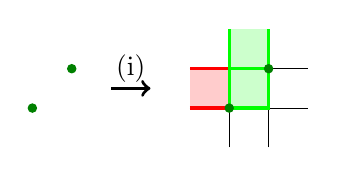
\begin{tikzpicture}[scale=.5]
\Vpoint{0}{0};
\Vpoint{1}{1};
\draw [very thick,->] (2,0.5) -- (3,0.5);
\draw (4,0) -- (7,0);
\draw (4,1) -- (7,1);
\draw (5,-1) -- (5,2);
\draw (6,-1) -- (6,2);
\zoneD{H};
\zoneE{V};
\zoneH{V};
\draw (5.5,-0.5) node {};
\Vpoint{5}{0};
\Vpoint{6}{1};
\etiquette{1};
\end{tikzpicture}
&
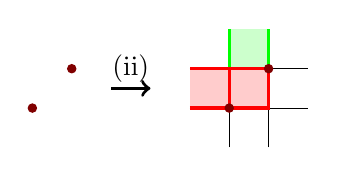
\begin{tikzpicture}[scale=.5]
\Hpoint{0}{0};
\Hpoint{1}{1};
\draw [very thick,->] (2,0.5) -- (3,0.5);
\draw (4,0) -- (7,0);
\draw (4,1) -- (7,1);
\draw (5,-1) -- (5,2);
\draw (6,-1) -- (6,2);
\zoneH{V};
\zoneD{H};
\zoneE{H};
\draw (6.5,0.5) node {};
\Hpoint{5}{0};
\Hpoint{6}{1};
\etiquette{2};
\end{tikzpicture}
&
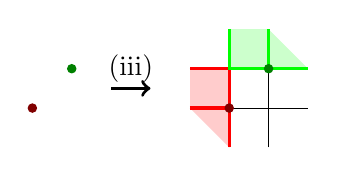
\begin{tikzpicture}[scale=.5]
\Hpoint{0}{0};
\Vpoint{1}{1};
\draw [very thick,->] (2,0.5) -- (3,0.5);
\draw (4,0) -- (7,0);
\draw (4,1) -- (7,1);
\draw (5,-1) -- (5,2);
\draw (6,-1) -- (6,2);
\zoneA{H};
\zoneD{H};
\zoneI{V};
\zoneH{V};
\Hpoint{5}{0};
\Vpoint{6}{1};
\etiquette{3};
\end{tikzpicture}
&
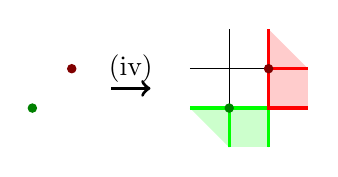
\begin{tikzpicture}[scale=.5]
\Vpoint{0}{0};
\Hpoint{1}{1};
\draw [very thick,->] (2,0.5) -- (3,0.5);
\draw (4,0) -- (7,0);
\draw (4,1) -- (7,1);
\draw (5,-1) -- (5,2);
\draw (6,-1) -- (6,2);
\zoneA{V};
\zoneB{V};
\zoneF{H};
\zoneI{H};
\Vpoint{5}{0};
\Hpoint{6}{1};
\etiquette{4};
\end{tikzpicture}
\\
\hline
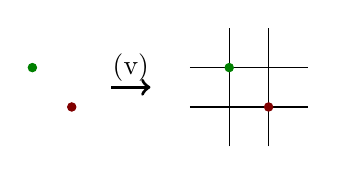
\begin{tikzpicture}[scale=.5]
\Vpoint{0}{1};
\Hpoint{1}{0};
\draw [very thick,->] (2,0.5) -- (3,0.5);
\draw (4,0) -- (7,0);
\draw (4,1) -- (7,1);
\draw (5,-1) -- (5,2);
\draw (6,-1) -- (6,2);
\draw (6.5,1.5) node {};
\Vpoint{5}{1};
\Hpoint{6}{0};
\etiquette{5};
\end{tikzpicture}
&
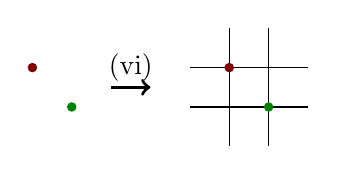
\begin{tikzpicture}[scale=.5]
\Hpoint{0}{1};
\Vpoint{1}{0};
\draw [very thick,->] (2,0.5) -- (3,0.5);
\draw (4,0) -- (7,0);
\draw (4,1) -- (7,1);
\draw (5,-1) -- (5,2);
\draw (6,-1) -- (6,2);
\draw (4.5,-0.5) node {};
\Hpoint{5}{1};
\Vpoint{6}{0};
\etiquette{6};
\end{tikzpicture}
&
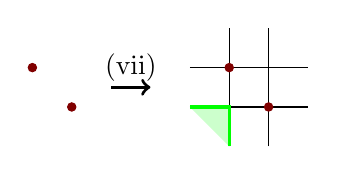
\begin{tikzpicture}[scale=.5]
\Hpoint{0}{1};
\Hpoint{1}{0};
\draw [very thick,->] (2,0.5) -- (3,0.5);
\draw (4,0) -- (7,0);
\draw (4,1) -- (7,1);
\draw (5,-1) -- (5,2);
\draw (6,-1) -- (6,2);
\zoneA{V};
\Hpoint{5}{1};
\Hpoint{6}{0};
\etiquette{7};
\end{tikzpicture}
&
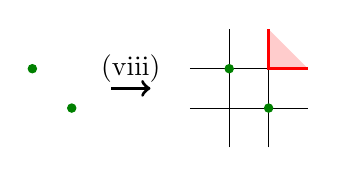
\begin{tikzpicture}[scale=.5]
\Vpoint{0}{1};
\Vpoint{1}{0};
\draw [very thick,->] (2,0.5) -- (3,0.5);
\draw (4,0) -- (7,0);
\draw (4,1) -- (7,1);
\draw (5,-1) -- (5,2);
\draw (6,-1) -- (6,2);
\zoneI{H};
\Vpoint{5}{1};
\Vpoint{6}{0};
\etiquette{8};
\end{tikzpicture}
\end{tabular}
\begin{center}
\caption{Rewriting rules }\label{fig:rewrite}
\end{center}
\end{figure}
For example rule  means that if two points  and  are in increasing order  and  and belong to  then every point  of the permutation must respect:
\begin{itemize}
\item If  then  and  belongs to .
\item If  and  then  belongs to .
\end{itemize}
\end{prop}

\begin{proof}
We prove that  is not valid \ssi  violates a rule of .
Suppose that  is not valid then  has one of the four colored patterns of Definition~\ref{def:validColoring}.
If  has a pattern \RRR then  violate rule  applied to elements  and  of the pattern \RRR, as element  of the pattern lies in a zone that should be empty.
If  has a pattern \GGG then  violate rule  applied to elements  and  of the pattern \GGG, as element  of the pattern lies in a zone that should be empty.
If  has a pattern \GGR then  violate rule  applied to elements of \G of the pattern \GGR.
If  has a pattern \RRG then  violate rule  applied to elements of \R of the pattern \RRG.
Conversely if  violates a rule of  then a comprehensive study shows that  has one of the four colored patterns of Definition~\ref{def:validColoring} and is not valid.
\end{proof}

We can use implication rules of  to limit the number of bicoloring to test, using the following idea: knowing the coloring of some points in the permutation (either in \R or in \G), the deduction rules given in Figure~\ref{fig:rewrite} can be applied until we obtain either a contradiction or no more rule can be applied. 
We can try the following algorithm: Set the color of two increasing points of , use implication rules to deduce the color of the other points and test whether the coloring obtained is right. 
Unfortunately, implication rules are not sufficient to ensure that given the color two points, the color of all other points is set. 
We may have to choose arbitrary the color of lots of points. 
To ensure that the number of bicoloring to test is polynomial, we have to study more precisely properties of increasing sequences in a valid bicoloring.

\begin{defn}
Let  be a bicoloring of a permutation . 
We call {\em \ascentRG} a pair of two points  such that , ,  and .
We define in the same way \ascentsGR, RR or GG.
\end{defn}



Rule  of  implies that every \ascentRG fixes the color of all points to the left of  below  (which are in \R) and to the right of  above  (which are in \G). 
The following theorem shows that when  is -indecomposable, the color of points to the left of  above  is also fixed.



\begin{thm}\label{thm:RGIncreasing}
Consider a valid coloring of a -decomposable permutation .
If there exist two points  such that  and , 
then the color of every point  with  or  is determined by iterations of rules {} knowing only the color of  and  
and can be represented as follows, the second diagram being a short representation of this alternance which will be used in the sequel. 
Furthermore, any increasing sequence  of points located either to the left of  or to the top of  is either monochromatic or colored .
Moreover, knowing  and , we can decide the color of the points whose indices are less than  or whose values are greater than  in linear time.
\end{thm}

\begin{figure}[H]
\begin{center}
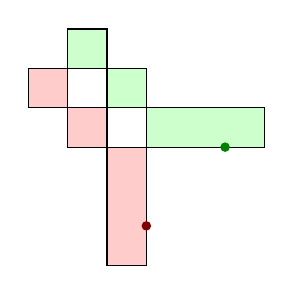
\begin{tikzpicture}[scale=.5]
\draw[Hfill] (-1,-1) rectangle (0,2);
\draw[Vfill] (0,2) rectangle (3,3);
\draw (-0.5,2.5) node {};
\Hpoint{0}{0};
\Vpoint{2}{2};
\draw (0.5,0) node{};
\draw (2,1.5) node{};
\begin{scope}
\draw[Hfill] (-2,2) rectangle (-1,3);
\draw [Vfill] (-1,3) rectangle (0,4);
\draw (-1.5,3.5) node {};
\end{scope}
\begin{scope}[shift={(-1,1)}]
\draw[Hfill] (-2,2) rectangle (-1,3);
\draw [Vfill] (-1,3) rectangle (0,4);
\draw (-1.6,3.8) node {};
\end{scope}
\end{tikzpicture}
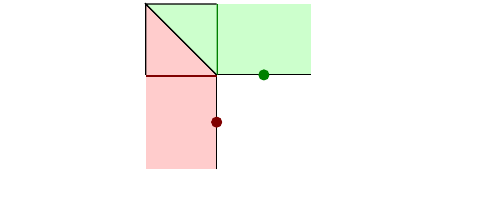
\begin{tikzpicture}[scale=.6]
\useasboundingbox (-3,1.5) (6,5);
\fill [Hfill] (-0.5,2) rectangle (1,4);
\fill [Vfill] (1,4) rectangle (3,5.5);
\draw (-0.5,4) -- (3,4);
\draw (1,2) -- (1,5.5);
\Hpoint{1}{3};
\draw (0.6,2.75) node {};
\Vpoint{2}{4};
\draw (2,4.4) node {};
\zoneRG{1}{4}{1.5}
\end{tikzpicture}

\caption{Zone }\label{fig:zoneRG}
\end{center}
\end{figure}

\begin{pf}
The proof is by induction on the {\em assigned} border between the zone not yet assigned to a stack and the {\em assigned} zone containing  and  where points are 
forced to be in a specific stack. 
At first, the {\em assigned} border is reduced to the segments  as well as the assigned zone (where ).

More formally we build sequences  and  such that  in an \ascentRG and the color of all points lying in the set  is determined and respects Figure~\ref{fig:zoneRG}.
We set  and .
We prove that if ( or ) then we can build  and  such that  or .

We set  and  (see Figure~\ref{fig:H0V0}). 
By rule (\rmnum{3}) applied to  and ,  and . 
Then, different situations may happen depending on whether areas  and  are empty:

\paragraph{ and  empty:} Then  is -decomposable which is in contradiction with our hypothesis.

\paragraph{ and  both non empty:} If both of the colored zones  or  are non empty, we set  and  (see Figure~\ref{fig:H0V0}). 
Then  is a partition of , where  (see Figure~\ref{fig:H0V0}). 
The only points of  whose color is not determined yet are those of . 
If  is not empty consider a point  of . 
If  then rule (\rmnum{1}) applied to  and  is in contradiction with the existence of . 
Hence  but then rule (\rmnum{2}) applied to  and  is in contradiction with the existence of . 
So  is empty and the color of all points of  is determined and respects Figure~\ref{fig:zoneRG}.

\begin{figure}[H]
\begin{center}
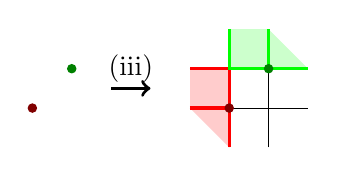
\begin{tikzpicture}[scale=.5]
\Hpoint{0}{0};
\Vpoint{1}{1};
\draw [very thick,->] (2,0.5) -- (3,0.5);
\draw (4,0) -- (7,0);
\draw (4,1) -- (7,1);
\draw (5,-1) -- (5,2);
\draw (6,-1) -- (6,2);
\zoneA{H};
\zoneD{H};
\zoneI{V};
\zoneH{V};
\Hpoint{5}{0};
\Vpoint{6}{1};
\etiquette{3};
\draw (4.5,-0.5) node {};
\draw (5.5,1.5) node {};
\end{tikzpicture}
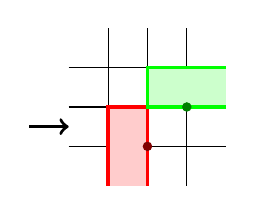
\begin{tikzpicture}[scale=.5]
\draw [very thick,->] (2,0.5) -- (3,0.5);
\draw (3,0) -- (7,0);
\draw (3,1) -- (7,1);
\draw (3,2) -- (7,2);
\draw (4,-1) -- (4,3);
\draw (5,-1) -- (5,3);
\draw (6,-1) -- (6,3);
\draw [H,Hfill,very thick] (4,-1) -- (4,1) -- (5,1) -- (5,-1);
\draw [V,Vfill,very thick] (7,1) -- (5,1) -- (5,2) -- (7,2);
\draw (3.5,-0.5) node {};
\draw (3.5,0.5) node {};
\draw (5.5,2.5) node {};
\draw (6.5,2.5) node {};
\draw (4.5,1.5) node {};
\Hpoint{5}{0};
\Vpoint{6}{1};
\end{tikzpicture}
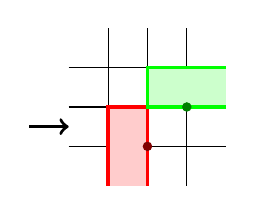
\begin{tikzpicture}[scale=.5]
\draw [very thick,->] (2,0.5) -- (3,0.5);
\draw (3,0) -- (7,0);
\draw (3,1) -- (7,1);
\draw (3,2) -- (7,2);
\draw (4,-1) -- (4,3);
\draw (5,-1) -- (5,3);
\draw (6,-1) -- (6,3);
\draw [H,Hfill,very thick] (4,-1) -- (4,1) -- (5,1) -- (5,-1);
\draw [V,Vfill,very thick] (7,1) -- (5,1) -- (5,2) -- (7,2);
\draw (3.5,-0.5) node {};
\draw (3.5,0.5) node {};
\draw (5.5,2.5) node {};
\draw (6.5,2.5) node {};
\draw (4.5,1.5) node {};
\Hpoint{5}{0};
\Vpoint{6}{1};
\end{tikzpicture}
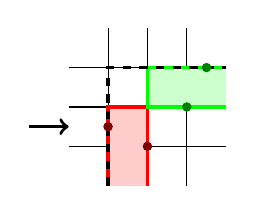
\begin{tikzpicture}[scale=.5]
\draw [very thick,->] (2,0.5) -- (3,0.5);
\draw (3,0) -- (7,0);
\draw (3,1) -- (7,1);
\draw (3,2) -- (7,2);
\draw (4,-1) -- (4,3);
\draw (5,-1) -- (5,3);
\draw (6,-1) -- (6,3);
\draw [H,Hfill,very thick] (4,-1) -- (4,1) -- (5,1) -- (5,-1);
\draw [V,Vfill,very thick] (7,1) -- (5,1) -- (5,2) -- (7,2);
\draw [very thick, dashed] (4,-1) -- (4,2) -- (7,2);
\draw (3.5,-0.5) node {};
\draw (3.5,0.5) node {};
\draw (5.5,2.5) node {};
\draw (6.5,2.5) node {};
\draw (4.5,1.5) node {};
\Hpoint{5}{0};
\Vpoint{6}{1};
\Hpoint{4}{0.5};
\Vpoint{6.5}{2};
\draw (4.5,0.5) node {{\small }};
\draw (6.5,1.7) node {{\small }};
\end{tikzpicture}
\caption{Transitive closure}\label{fig:H0V0}
\end{center}
\end{figure}

\paragraph{Only one area in  and  is empty:}
The same proof as the preceding case allow us to define a new point  or  depending on which area is empty and we can extend the {\em assigned} border as shown in next figure.
\begin{center}
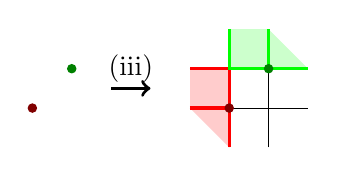
\begin{tikzpicture}[scale=.5]
\Hpoint{0}{0};
\Vpoint{1}{1};
\draw [very thick,->] (2,0.5) -- (3,0.5);
\draw (4,0) -- (7,0);
\draw (4,1) -- (7,1);
\draw (5,-1) -- (5,2);
\draw (6,-1) -- (6,2);
\zoneA{H};
\zoneD{H};
\zoneI{V};
\zoneH{V};
\Hpoint{5}{0};
\Vpoint{6}{1};
\etiquette{3};
\draw (4.5,-0.5) node {};
\draw (5.5,1.5) node {};
\end{tikzpicture}
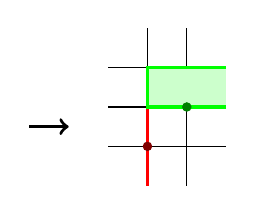
\begin{tikzpicture}[scale=.5]
\draw [very thick,->] (2,0.5) -- (3,0.5);
\draw (4,0) -- (7,0);
\draw (4,1) -- (7,1);
\draw (4,2) -- (7,2);
\draw (5,-1) -- (5,3);
\draw (6,-1) -- (6,3);
\draw [H,Hfill,very thick] (5,-1) -- (5,1) -- (5,1) -- (5,-1);
\draw [V,Vfill,very thick] (7,1) -- (5,1) -- (5,2) -- (7,2);
\draw (4.5,-0.5) node {};
\draw (4.5,0.5) node {};
\draw (5.5,2.5) node {};
\draw (6.5,2.5) node {};
\Hpoint{5}{0};
\Vpoint{6}{1};
\end{tikzpicture}
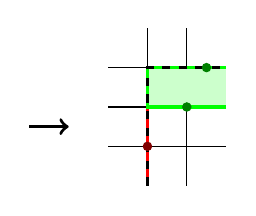
\begin{tikzpicture}[scale=.5]
\draw [very thick,->] (2,0.5) -- (3,0.5);
\draw (4,0) -- (7,0);
\draw (4,1) -- (7,1);
\draw (4,2) -- (7,2);
\draw (5,-1) -- (5,3);
\draw (6,-1) -- (6,3);
\draw [H,Hfill,very thick] (5,-1) -- (5,1) -- (5,1) -- (5,-1);
\draw [V,Vfill,very thick] (7,1) -- (5,1) -- (5,2) -- (7,2);
\draw (4.5,-0.5) node {};
\draw (4.5,0.5) node {};
\draw (5.5,2.5) node {};
\draw (6.5,2.5) node {};
\draw [very thick, dashed] (5,-1) -- (5,2) -- (7,2);
\Hpoint{5}{0};
\Vpoint{6}{1};
\Vpoint{6.5}{2};
\draw (6.5,1.7) node {{\small }};
\end{tikzpicture}
\begin{center}
{Transitive closure}
\end{center}
\end{center}

Hence, the {\em assigned} zone keeps growing until all permutation points are assigned, proving Theorem~\ref{thm:RGIncreasing}.
\end{pf}


We also have a similar result extending rule :

\begin{thm}\label{thm:GRIncreasing}
Consider a valid coloring of a -decomposable permutation .
If there exist two points  such that  and ,
then the color of each point  with  or  is determined. 
Such a zone will be represented as 
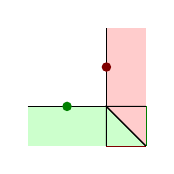
\begin{tikzpicture}[scale=.5]
\useasboundingbox (1,0) (4,3);
\fill [Vfill] (1,0) rectangle (3,1);
\fill [Hfill] (3,1) rectangle (4,3);
\draw (1,1) -- (4,1);
\draw (3,0) -- (3,3);
\Hpoint{3}{2};
\draw (3.5,1.7) node {{\tiny }};
\Vpoint{2}{1};
\draw (2,0.7) node {{\tiny }};
\zoneGR{4}{0}{1};
\end{tikzpicture} in the sequel.
\end{thm}
\begin{pf}
Notice that rules are symetric so that the same proof as for Theorem~\ref{thm:RGIncreasing} holds.
\end{pf}


Knowing Theorem~\ref{thm:RGIncreasing} and Theorem~\ref{thm:GRIncreasing}, to set the color of as much points as possible, we better have to choose the lower right \ascentRG or the upper left \ascentGR. 
Let us now define properly these particular ascents.

We consider a valid bicoloring  of a permutation .
We define  as the set of \ascentsRG of .

\begin{lem}
Suppose . 
Among \ascentsRG of , the pair  which maximizes  first then minimizes  (for  fixed) is the same than the pair that minimizes  first then maximizes  (for  fixed).
\end{lem}
\begin{proof}
Let  be the pair that maximizes  first then minimizes  and  be the pair that minimizes  first then maximizes . 
Then by definition  and .

If  then  is an \ascentGG and rule  is in contradiction with  as .
If  then  is an \ascentRR and rule  is in contradiction with  as . 
Hence  is an \ascentRG.
Then by definition of ,  and by definition of , . 
So .
\end{proof}

By the preceding lemma, when  we can define  as the lower right \ascentRG. 
By symmetry, we can also define  the upper left \ascentGR when , where  is the set similar to  but for \ascentsGR.


Now we have all the tools to prove that there are only a polynomial number of bicolorings to test. 
We juste have to do a case study depending on  or  are empty.


\subsection{Case study}

Recall that from Proposition~\ref{prop:pushallMoinsDecomposable} if  is -decomposable then  is -stack pushall sortable 
if and only if each -indecomposable block of  is -stack pushall sortable.
Thus, we can assume that  is -indecomposable.

In this section, we consider a valid coloring  of a -indecomposable permutation .
We prove that knowing if there are ascents RG or GR in  and knowing , ,  and  (if they exist), we can deduce the color of every point of .

We prove this considering  cases depending on whether there are ascents RG or GR in .


\subsubsection{There is no bicolored ascents}

If  and  are both empty, then the coloring is monochromatic:
\begin{prop}\label{prop:monochromatic}
Let  be a -indecomposable permutation and  a valid coloring of  such that every pattern  of  is monochromatic. 
Then all points of  have the same color.
\end{prop}
\begin{pf}
Let  and  be two consecutive left-to-right minima of . 
By definition there are no point below  and to the left of  as shown by the empty sign in the following figure
\begin{tikzpicture}[scale=.3]
\draw (0,2) -- (4,2);
\draw (2,0) -- (2,4);
\draw (1,1) node {};
\draw (1,2) [fill] circle (3pt);
\draw (1,2.4) node {{\scriptsize }};
\draw (2,1) [fill] circle (3pt);
\draw (2.5,1) node {{\scriptsize }};
\draw (3,3) [fill] circle (3pt);
\draw (3.3,3.3) node {{\scriptsize }};
\end{tikzpicture}.
As  is -indecomposable, there exist a point  above  and to the right of . 
As increasing subsequences are monochromatic,  and  have the same color. 
The same goes for  and . Thus  and  have the same color. 
So all left-to-right minima of  have the same color.
By definition of left-to-right minima, for every non-minimal point  there exists a left-to-right minima  such that  is a pattern  of . 
Thus  has the same color as , and all points of  have the same color.
\end{pf}


\subsubsection{There is no \ascentRG but some \ascentsGR}

We suppose in this section that there exists at least one \ascentGR but no \ascentRG.
As  is non empty,  and  are defined.
We prove that once  and  are determined, then it fixes the color of every other point of the permutation.

\begin{prop}\label{prop:diagrammesGR}
Let  be a -indecomposable permutation and  a valid coloring of  such that there is no increasing subsequence RG in  and there is at least an increasing sequence GR in . 
Then  has one of the following shapes (where maybe  or ):

\begin{center}
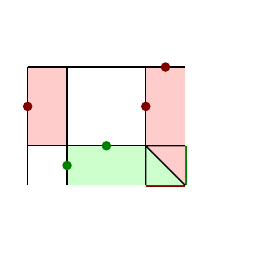
\begin{tikzpicture}[scale=.5]
\useasboundingbox (0,-1) (5,4);
\fill [Vfill] (1,0) rectangle (3,1);
\fill [Hfill] (0,1) rectangle (1,3);
\fill [Hfill] (3,1) rectangle (4,3);
\draw (0,1) -- (4,1);
\draw (0,3) -- (4,3);
\draw (0,0) -- (0,3);
\draw (1,0) -- (1,3);
\draw (3,0) -- (3,3);
\draw (2,2) node {};
\draw (0.5,0.5) node {};
\Hpoint{3}{2};
\draw (3.5,1.7) node {{\tiny }};
\Vpoint{2}{1};
\draw (2,0.7) node {{\tiny }};
\Vpoint{1}{0.5};
\draw (1.3,0.3) node {{\tiny }};
\Hpoint{3.5}{3};
\draw (3.45,2.65) node {{\tiny }};
\Hpoint{0}{2};
\draw (0.4,2) node {{\tiny }};
\zoneGR{4}{0}{1};
\end{tikzpicture}
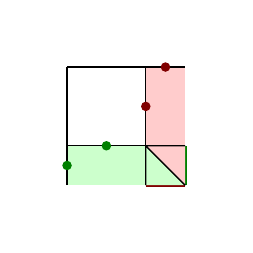
\begin{tikzpicture}[scale=.5]
\useasboundingbox (0,-1) (5,4);
\fill [Vfill] (1,0) rectangle (3,1);
\fill [Hfill] (3,1) rectangle (4,3);
\draw (1,1) -- (4,1);
\draw (1,3) -- (4,3);
\draw (1,0) -- (1,3);
\draw (3,0) -- (3,3);
\draw (2,2) node {};
\Hpoint{3}{2};
\draw (3.5,1.7) node {{\tiny }};
\Vpoint{2}{1};
\draw (2,0.7) node {{\tiny }};
\Vpoint{1}{0.5};
\draw (1.3,0.3) node {{\tiny }};
\Hpoint{3.5}{3};
\draw (3.45,2.65) node {{\tiny }};
\zoneGR{4}{0}{1};
\end{tikzpicture}
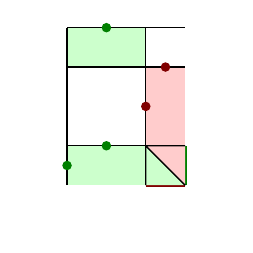
\begin{tikzpicture}[scale=.5]
\useasboundingbox (0,-1) (5,4);
\fill [Vfill] (1,0) rectangle (3,1);
\fill [Hfill] (3,1) rectangle (4,3);
\fill [Vfill] (1,3) rectangle (3,4);
\draw (1,1) -- (4,1);
\draw (1,3) -- (4,3);
\draw (1,4) -- (4,4);
\draw (1,0) -- (1,4);
\draw (3,0) -- (3,4);
\draw (3.5,3.5) node {};
\draw (2,2) node {};
\Hpoint{3}{2};
\draw (3.5,1.7) node {{\tiny }};
\Vpoint{2}{1};
\draw (2,0.7) node {{\tiny }};
\Vpoint{1}{0.5};
\draw (1.3,0.3) node {{\tiny }};
\Hpoint{3.5}{3};
\draw (3.45,2.65) node {{\tiny }};
\Vpoint{2}{4};
\draw (2,3.7) node {{\tiny }};
\zoneGR{4}{0}{1};
\end{tikzpicture}
\end{center}
\end{prop}

\begin{rem}
Here and in all the following, when a zone of a diagram is colored with \R (resp. \G), it means than if there are some points lying in this zone, they are in \R (resp. \G). And when a zone of a diagram has an empty sign, it means than this zone is empty.
\end{rem}

\begin{pf}
The color of every point  such that  or  is determined by Theorem~\ref{thm:GRIncreasing} (see the first diagram of Figure~\ref{fig:tikzGR1}).
Note that we denote by  the zone where the color of the points is unknown.
By maximality of , any point above  and lower left with respect to  is in \R. By minimality of , any point to the left of  and top right with respect to  is in \G. As no point can be both in \R and in \G, we know that the zone between  and  is empty, as shown in the second diagram of Figure~\ref{fig:tikzGR1}.

\begin{figure}[H]
\begin{center}
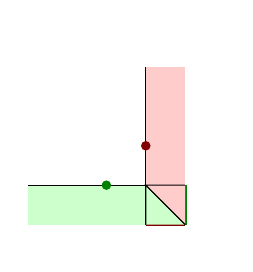
\begin{tikzpicture}[scale=.5]
\useasboundingbox (0,-0.5) (5,5);
\fill [Vfill] (0,0) rectangle (3,1);
\fill [Hfill] (3,1) rectangle (4,4);
\draw (0,1) -- (4,1);
\draw (3,0) -- (3,4);
\Hpoint{3}{2};
\draw (3.5,1.7) node {{\tiny }};
\Vpoint{2}{1};
\draw (2,0.7) node {{\tiny }};
\draw (1.5,2.5) node {};
\zoneGR{4}{0}{1};
\end{tikzpicture}
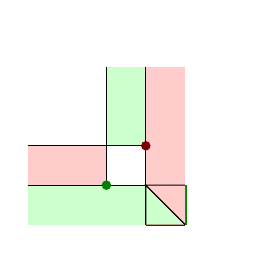
\begin{tikzpicture}[scale=.5]
\useasboundingbox (0,-0.5) (5,5);
\fill [Vfill] (0,0) rectangle (3,1);
\fill [Hfill] (0,1) rectangle (2,2);
\fill [Hfill] (3,1) rectangle (4,4);
\fill [Vfill] (2,2) rectangle (3,4);
\draw (0,1) -- (4,1);
\draw (0,2) -- (3,2);
\draw (2,1) -- (2,4);
\draw (3,0) -- (3,4);
\draw (2.5,1.5) node {};
\Hpoint{3}{2};
\draw (3.5,1.7) node {{\tiny }};
\Vpoint{2}{1};
\draw (2,0.7) node {{\tiny }};
\draw (1,3) node {};
\zoneGR{4}{0}{1};
\end{tikzpicture}
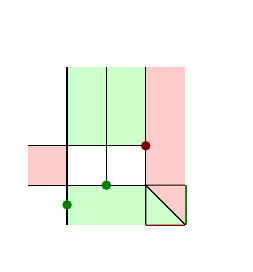
\begin{tikzpicture}[scale=.5]
\useasboundingbox (0,-0.5) (5,5);
\fill [Vfill] (1,0) rectangle (3,1);
\fill [Hfill] (0,1) rectangle (1,2);
\fill [Hfill] (3,1) rectangle (4,4);
\fill [Vfill] (1,2) rectangle (3,4);
\draw (0,1) -- (4,1);
\draw (0,2) -- (3,2);
\draw (2,1) -- (2,4);
\draw (1,0) -- (1,4);
\draw (3,0) -- (3,4);
\draw (2.5,1.5) node {};
\draw (1.5,1.5) node {};
\draw (0.5,0.5) node {};
\Hpoint{3}{2};
\draw (3.5,1.7) node {{\tiny }};
\Vpoint{2}{1};
\draw (2,0.7) node {{\tiny }};
\Vpoint{1}{0.5};
\draw (1.3,0.3) node {{\tiny }};
\draw (0.5,3) node {};
\zoneGR{4}{0}{1};
\end{tikzpicture}
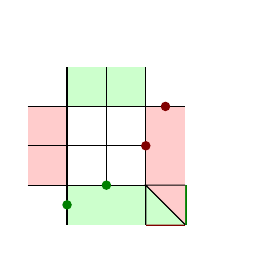
\begin{tikzpicture}[scale=.5]
\useasboundingbox (0,-0.5) (5,5);
\fill [Vfill] (1,0) rectangle (3,1);
\fill [Hfill] (0,1) rectangle (1,3);
\fill [Hfill] (3,1) rectangle (4,3);
\fill [Vfill] (1,3) rectangle (3,4);
\draw (0,1) -- (4,1);
\draw (0,2) -- (3,2);
\draw (0,3) -- (4,3);
\draw (2,1) -- (2,4);
\draw (1,0) -- (1,4);
\draw (3,0) -- (3,4);
\draw (3.5,3.5) node {};
\draw (2.5,2.5) node {};
\draw (1.5,2.5) node {};
\draw (2.5,1.5) node {};
\draw (1.5,1.5) node {};
\draw (0.5,0.5) node {};
\Hpoint{3}{2};
\draw (3.5,1.7) node {{\tiny }};
\Vpoint{2}{1};
\draw (2,0.7) node {{\tiny }};
\Vpoint{1}{0.5};
\draw (1.3,0.3) node {{\tiny }};
\Hpoint{3.5}{3};
\draw (3.45,2.65) node {{\tiny }};
\draw (0.5,3.5) node {};
\zoneGR{4}{0}{1};
\end{tikzpicture}
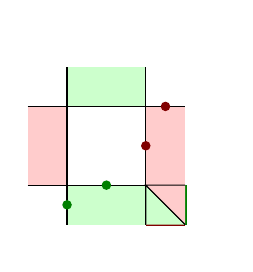
\begin{tikzpicture}[scale=.5]
\useasboundingbox (0,-0.5) (5,5);
\fill [Vfill] (1,0) rectangle (3,1);
\fill [Hfill] (0,1) rectangle (1,3);
\fill [Hfill] (3,1) rectangle (4,3);
\fill [Vfill] (1,3) rectangle (3,4);
\draw (0,1) -- (4,1);
\draw (0,3) -- (4,3);
\draw (1,0) -- (1,4);
\draw (3,0) -- (3,4);
\draw (3.5,3.5) node {};
\draw (2,2) node {};
\draw (0.5,0.5) node {};
\Hpoint{3}{2};
\draw (3.5,1.7) node {{\tiny }};
\Vpoint{2}{1};
\draw (2,0.7) node {{\tiny }};
\Vpoint{1}{0.5};
\draw (1.3,0.3) node {{\tiny }};
\Hpoint{3.5}{3};
\draw (3.45,2.65) node {{\tiny }};
\draw (0.5,3.5) node {};
\draw (0.5,2) node {};
\draw (2,3.5) node {};
\zoneGR{4}{0}{1};
\end{tikzpicture}

\caption{Only bicolored increasing subsequences GR exist}\label{fig:tikzGR1}
\end{center}
\end{figure}

Let  be the leftmost point among points below  (notice that  may be equal to ). Applying rule (\rmnum{1}) to  and , we obtain the third diagram (note that if  the column between  and  does not exist). Let  be the topmost point to the right of  ( may be equal to ). Applying rule (\rmnum{2}) to  and , we obtain the fourth diagram of Figure~\ref{fig:tikzGR1} (if  the column between  and  does not exist).

At last, we number two different areas and discuss about the different cases whether these zones are empty or not. These zones are pictured in the fifth diagram of Figure~\ref{fig:tikzGR1}.



\paragraph{Zone  is not empty}

Let  be the leftmost point inside zone . Note that  may be above or below . First diagram of Figure~\ref{fig:tikz1nonVide} illustrates the position of point . Applying rule (\rmnum{2}) to  and  we obtain the second diagram of Figure~\ref{fig:tikz1nonVide}.
By hypothesis, there are no increasing sequence RG, thus there are no points in \G in the up-right quadrant of . This leads to the third diagram.
At last, if the zone  is not empty, then  is -decomposable by cutting along the row of  and the column of . Thus  is empty and all points have a determined color, as in the first diagram of Proposition~\ref{prop:diagrammesGR}.


\begin{figure}[H]
\begin{center}
\begin{tikzpicture}[scale=.5]
\useasboundingbox (-1,-0.5) (5,5);
\fill [Vfill] (1,0) rectangle (3,1);
\fill [Hfill] (0,1) rectangle (1,3);
\fill [Hfill] (3,1) rectangle (4,3);
\fill [Vfill] (1,3) rectangle (3,4);
\draw (-1,1) -- (4,1);
\draw (-1,3) -- (4,3);
\draw (0,0) -- (0,4);
\draw (1,0) -- (1,4);
\draw (3,0) -- (3,4);
\draw (3.5,3.5) node {};
\draw (2,2) node {};
\draw (0.5,0.5) node {};
\draw (-0.5,0.5) node {};
\draw (-0.5,2) node {};
\Hpoint{3}{2};
\draw (3.5,1.7) node {{\tiny }};
\Vpoint{2}{1};
\draw (2,0.7) node {{\tiny }};
\Vpoint{1}{0.5};
\draw (1.3,0.3) node {{\tiny }};
\Hpoint{3.5}{3};
\draw (3.45,2.65) node {{\tiny }};
\Hpoint{0}{2};
\draw (0.4,2) node {{\tiny }};
\draw (0.5,3.5) node {};
\draw (-0.5,3.5) node {};
\zoneGR{4}{0}{1};
\end{tikzpicture}
\begin{tikzpicture}[scale=.5]
\useasboundingbox (-1,-0.5) (5,5);
\fill [Vfill] (1,0) rectangle (3,1);
\fill [Hfill] (0,1) rectangle (1,3);
\fill [Hfill] (3,1) rectangle (4,3);
\fill [Vfill] (0,3) rectangle (3,4);
\draw (-1,1) -- (4,1);
\draw (-1,3) -- (4,3);
\draw (0,0) -- (0,4);
\draw (1,0) -- (1,4);
\draw (3,0) -- (3,4);
\draw (3.5,3.5) node {};
\draw (2,2) node {};
\draw (0.5,0.5) node {};
\draw (-0.5,0.5) node {};
\draw (-0.5,2) node {};
\Hpoint{3}{2};
\draw (3.5,1.7) node {{\tiny }};
\Vpoint{2}{1};
\draw (2,0.7) node {{\tiny }};
\Vpoint{1}{0.5};
\draw (1.3,0.3) node {{\tiny }};
\Hpoint{3.5}{3};
\draw (3.45,2.65) node {{\tiny }};
\Hpoint{0}{2};
\draw (0.4,2) node {{\tiny }};
\draw (-0.5,3.5) node {};
\zoneGR{4}{0}{1};
\end{tikzpicture}
\begin{tikzpicture}[scale=.5]
\useasboundingbox (-1,-0.5) (5,5);
\fill [Vfill] (1,0) rectangle (3,1);
\fill [Hfill] (0,1) rectangle (1,3);
\fill [Hfill] (3,1) rectangle (4,3);
\draw (-1,1) -- (4,1);
\draw (-1,3) -- (4,3);
\draw (0,0) -- (0,4);
\draw (1,0) -- (1,4);
\draw (3,0) -- (3,4);
\draw (3.5,3.5) node {};
\draw (2,2) node {};
\draw (0.5,0.5) node {};
\draw (-0.5,0.5) node {};
\draw (-0.5,2) node {};
\draw (0.5,3.5) node {};
\draw (2,3.5) node {};
\Hpoint{3}{2};
\draw (3.5,1.7) node {{\tiny }};
\Vpoint{2}{1};
\draw (2,0.7) node {{\tiny }};
\Vpoint{1}{0.5};
\draw (1.3,0.3) node {{\tiny }};
\Hpoint{3.5}{3};
\draw (3.45,2.65) node {{\tiny }};
\Hpoint{0}{2};
\draw (0.4,2) node {{\tiny }};
\draw (-0.5,3.5) node {};
\zoneGR{4}{0}{1};
\end{tikzpicture}
\begin{tikzpicture}[scale=.5]
\useasboundingbox (0,-0.5) (5,4);
\fill [Vfill] (1,0) rectangle (3,1);
\fill [Hfill] (0,1) rectangle (1,3);
\fill [Hfill] (3,1) rectangle (4,3);
\draw (0,1) -- (4,1);
\draw (0,3) -- (4,3);
\draw (0,0) -- (0,3);
\draw (1,0) -- (1,3);
\draw (3,0) -- (3,3);
\draw (2,2) node {};
\draw (0.5,0.5) node {};
\Hpoint{3}{2};
\draw (3.5,1.7) node {{\tiny }};
\Vpoint{2}{1};
\draw (2,0.7) node {{\tiny }};
\Vpoint{1}{0.5};
\draw (1.3,0.3) node {{\tiny }};
\Hpoint{3.5}{3};
\draw (3.45,2.65) node {{\tiny }};
\Hpoint{0}{2};
\draw (0.4,2) node {{\tiny }};
\zoneGR{4}{0}{1};
\end{tikzpicture}

\caption{Zone  is not empty\label{fig:tikz1nonVide}}
\end{center}
\end{figure}

\paragraph{Zone  is empty}

Suppose that zone  is empty. If zone  is also empty then as  is -indecomposable, zone  is also empty and all points have a determined color, as in the second diagram of Proposition~\ref{prop:diagrammesGR}.

\begin{figure}[H]
\begin{center}
\begin{tikzpicture}[scale=.5]
\useasboundingbox (0,-0.5) (5,5);
\fill [Vfill] (1,0) rectangle (3,1);
\fill [Hfill] (3,1) rectangle (4,3);
\fill [Vfill] (1,3) rectangle (3,4);
\draw (0,1) -- (4,1);
\draw (0,3) -- (4,3);
\draw (1,0) -- (1,4);
\draw (3,0) -- (3,4);
\draw (3.5,3.5) node {};
\draw (2,2) node {};
\draw (0.5,2) node {};
\draw (0.5,0.5) node {};
\Hpoint{3}{2};
\draw (3.5,1.7) node {{\tiny }};
\Vpoint{2}{1};
\draw (2,0.7) node {{\tiny }};
\Vpoint{1}{0.5};
\draw (1.3,0.3) node {{\tiny }};
\Hpoint{3.5}{3};
\draw (3.45,2.65) node {{\tiny }};
\draw (0.5,3.5) node {};
\draw (2,3.5) node {};
\zoneGR{4}{0}{1};
\end{tikzpicture}
\begin{tikzpicture}[scale=.5]
\useasboundingbox (0,-0.5) (5,6);
\fill [Vfill] (1,0) rectangle (3,1);
\fill [Hfill] (3,1) rectangle (4,3);
\fill [Vfill] (1,3) rectangle (3,4);
\draw (0,1) -- (4,1);
\draw (0,3) -- (4,3);
\draw (0,4) -- (4,4);
\draw (1,0) -- (1,5);
\draw (3,0) -- (3,5);
\draw (3.5,3.5) node {};
\draw (2,2) node {};
\draw (0.5,2) node {};
\draw (0.5,0.5) node {};
\draw (2,4.5) node {};
\draw (3.5,4.5) node {};
\Hpoint{3}{2};
\draw (3.5,1.7) node {{\tiny }};
\Vpoint{2}{1};
\draw (2,0.7) node {{\tiny }};
\Vpoint{1}{0.5};
\draw (1.3,0.3) node {{\tiny }};
\Hpoint{3.5}{3};
\draw (3.45,2.65) node {{\tiny }};
\Vpoint{2}{4};
\draw (2,3.7) node {{\tiny }};
\draw (0.5,3.5) node {};
\draw (0.5,4.5) node {};
\zoneGR{4}{0}{1};
\end{tikzpicture}
\begin{tikzpicture}[scale=.5]
\useasboundingbox (0,-0.5) (5,6);
\fill [Vfill] (1,0) rectangle (3,1);
\fill [Hfill] (3,1) rectangle (4,3);
\fill [Vfill] (1,3) rectangle (3,4);
\fill [Hfill] (0,3) rectangle (1,4);
\draw (0,1) -- (4,1);
\draw (0,3) -- (4,3);
\draw (0,4) -- (4,4);
\draw (1,0) -- (1,5);
\draw (3,0) -- (3,5);
\draw (3.5,3.5) node {};
\draw (2,2) node {};
\draw (0.5,2) node {};
\draw (0.5,0.5) node {};
\draw (2,4.5) node {};
\draw (3.5,4.5) node {};
\Hpoint{3}{2};
\draw (3.5,1.7) node {{\tiny }};
\Vpoint{2}{1};
\draw (2,0.7) node {{\tiny }};
\Vpoint{1}{0.5};
\draw (1.3,0.3) node {{\tiny }};
\Hpoint{3.5}{3};
\draw (3.45,2.65) node {{\tiny }};
\Vpoint{2}{4};
\draw (2,3.7) node {{\tiny }};
\draw (0.5,4.5) node {};
\zoneGR{4}{0}{1};
\end{tikzpicture}
\begin{tikzpicture}[scale=.5]
\useasboundingbox (0,-0.5) (5,6);
\fill [Vfill] (1,0) rectangle (3,1);
\fill [Hfill] (3,1) rectangle (4,3);
\fill [Vfill] (1,3) rectangle (3,4);
\draw (0,1) -- (4,1);
\draw (0,3) -- (4,3);
\draw (0,4) -- (4,4);
\draw (1,0) -- (1,5);
\draw (3,0) -- (3,5);
\draw (3.5,3.5) node {};
\draw (2,2) node {};
\draw (0.5,2) node {};
\draw (0.5,0.5) node {};
\draw (2,4.5) node {};
\draw (3.5,4.5) node {};
\Hpoint{3}{2};
\draw (3.5,1.7) node {{\tiny }};
\Vpoint{2}{1};
\draw (2,0.7) node {{\tiny }};
\Vpoint{1}{0.5};
\draw (1.3,0.3) node {{\tiny }};
\Hpoint{3.5}{3};
\draw (3.45,2.65) node {{\tiny }};
\Vpoint{2}{4};
\draw (2,3.7) node {{\tiny }};
\draw (0.5,4.5) node {};
\draw (0.5,3.5) node {};
\zoneGR{4}{0}{1};
\end{tikzpicture}
\begin{tikzpicture}[scale=.5]
\useasboundingbox (0,-0.5) (5,4);
\fill [Vfill] (1,0) rectangle (3,1);
\fill [Hfill] (3,1) rectangle (4,3);
\fill [Vfill] (1,3) rectangle (3,4);
\draw (1,1) -- (4,1);
\draw (1,3) -- (4,3);
\draw (1,4) -- (4,4);
\draw (1,0) -- (1,4);
\draw (3,0) -- (3,4);
\draw (3.5,3.5) node {};
\draw (2,2) node {};
\Hpoint{3}{2};
\draw (3.5,1.7) node {{\tiny }};
\Vpoint{2}{1};
\draw (2,0.7) node {{\tiny }};
\Vpoint{1}{0.5};
\draw (1.3,0.3) node {{\tiny }};
\Hpoint{3.5}{3};
\draw (3.45,2.65) node {{\tiny }};
\Vpoint{2}{4};
\draw (2,3.7) node {{\tiny }};
\zoneGR{4}{0}{1};
\end{tikzpicture}
\caption{Zone  is empty\label{fig:tikz1Vide}}
\end{center}
\end{figure}

Otherwise, zone  is not empty and let  be the topmost point inside zone  ( may be to the left or to the right of ). This is depicted in the second diagram of Figure~\ref{fig:tikz1Vide}. We apply rule (\rmnum{1}) to  and  to obtain the third diagram. As there is no increasing subsequence RG, there is no point of \R in the lower left quadrant of  as depicted in the fourth diagram. Moreover,  is -indecomposable, thus zone  is empty and each point has a determined color, as in the last diagram of Proposition~\ref{prop:diagrammesGR}.
\end{pf}

\begin{defn}\label{def:C_GR}
Let  be a permutation and  and  two indices of  such that  is an ascent.
Set  and  such that .
We define  as the partial bicoloring of  having the following shape:

\begin{tikzpicture}[scale=.5]
\useasboundingbox (0,-1) (5,4.5);
\fill [Vfill] (1,0) rectangle (3,1);
\fill [Hfill] (0,1) rectangle (1,3);
\fill [Hfill] (3,1) rectangle (4,3);
\fill [Vfill] (1,3) rectangle (3,4);
\draw (1,0) -- (1,4);
\draw (3,0) -- (3,4);
\draw (0,1) -- (4,1);
\draw (0,3) -- (4,3);
\Hpoint{3}{2};
\draw (3.5,1.7) node {{\tiny }};
\Vpoint{2}{1};
\draw (2,0.7) node {{\tiny }};
\Vpoint{1}{0.5};
\draw (1.3,0.3) node {{\tiny }};
\Hpoint{3.5}{3};
\draw (3.45,2.65) node {{\tiny }};
\zoneGR{4}{0}{1};
\end{tikzpicture}
\end{defn}


\begin{prop}\label{prop:C_GR}
Let  be a -indecomposable permutation and  a valid coloring of  such that there is no increasing subsequence RG in  and there is at least an increasing sequence GR in . 
Then .
\end{prop}

\begin{pf}
This is a direct consequence of Proposition~\ref{prop:diagrammesGR} and Definition~\ref{def:C_GR}.
\end{pf}


\subsubsection{All bicolored increasing sequences are labeled }

We suppose in this section that there exists at least one \ascentRG but no \ascentGR.
As  is non empty,  and  are defined.
We prove that once  and  are determined, then it fixes the color of every other point of the permutation.

\begin{prop}\label{prop:diagrammesRG}
Let  be a -indecomposable permutation and  a valid coloring of  such that there is no increasing subsequence GR in  and there is at least an increasing sequence RG in . 
Then  has one of the following shapes (where maybe  or ):

\begin{center}
\begin{tikzpicture}[scale=.5]
\useasboundingbox (0,-1) (5,6);
\fill [Hfill] (0,2) rectangle (1,4);
\fill [Vfill] (1,4) rectangle (3,5);
\draw (0,4) -- (3,4);
\draw (1,3) -- (3,3);
\draw (0,2) -- (3,2);
\draw (1,2) -- (1,5);
\draw (2,2) -- (2,4);
\draw (3,2) -- (3,5);
\draw (2.5,3.5) node {};
\draw (2.5,2.5) node {};
\draw (1.5,2.5) node {};
\draw (1.5,3.5) node {};
\Hpoint{1}{3};
\draw (0.5,2.75) node {{\tiny }};
\Vpoint{2}{4};
\draw (2,4.5) node {{\tiny }};
\zoneRG{1}{4}{1}
\end{tikzpicture}
\begin{tikzpicture}[scale=.5]
\useasboundingbox (0,-1) (5,6);
\fill [Hfill] (0,2) rectangle (1,4);
\fill [Vfill] (1,4) rectangle (3,5);
\fill [Vfill] (1,1) rectangle (2,2);
\draw (0,4) -- (3,4);
\draw (1,3) -- (3,3);
\draw (0,2) -- (3,2);
\draw (0,1) -- (3,1);
\draw (1,1) -- (1,5);
\draw (2,1) -- (2,4);
\draw (3,1) -- (3,5);
\draw (2.5,3.5) node {};
\draw (2.5,2.5) node {};
\draw (0.5,1.5) node {};
\draw (2.5,1.5) node {};
\draw (1.5,2.5) node {};
\draw (1.5,3.5) node {};
\Hpoint{1}{3};
\draw (0.5,2.75) node {{\tiny }};
\Vpoint{2}{4};
\draw (2,4.5) node {{\tiny }};
\Vpoint{3}{4.5};
\draw (3.3,4.3) node {{\tiny }};
\Hpoint{0.5}{2};
\draw (0.3,2.3) node {{\tiny }};
\Vpoint{1.5}{1};
\draw (1.2,0.8) node {{\tiny }};
\zoneRG{1}{4}{1}
\end{tikzpicture}
\begin{tikzpicture}[scale=.5]
\useasboundingbox (0,-1) (6,6);
\fill [Hfill] (0,2) rectangle (1,4);
\fill [Vfill] (1,4) rectangle (3,5);
\fill [Vfill] (1,1) rectangle (2,2);
\fill [Vfill] (3,1) rectangle (4,2);
\draw (0,4) -- (4,4);
\draw (1,3) -- (4,3);
\draw (0,2) -- (4,2);
\draw (0,1) -- (4,1);
\draw (1,1) -- (1,5);
\draw (2,1) -- (2,4);
\draw (3,1) -- (3,5);
\draw (4,1) -- (4,5);
\draw (2.5,3.5) node {};
\draw (2.5,2.5) node {};
\draw (0.5,1.5) node {};
\draw (2.5,1.5) node {};
\draw (1.5,2.5) node {};
\draw (1.5,3.5) node {};
\draw (3.5,2.5) node {};
\draw (3.5,3.5) node {};
\draw (3.5,4.5) node {};
\Hpoint{1}{3};
\draw (0.5,2.75) node {{\tiny }};
\Vpoint{2}{4};
\draw (2,4.5) node {{\tiny }};
\Vpoint{3}{4.5};
\draw (3.2,4.2) node {{\tiny }};
\Hpoint{0.5}{2};
\draw (0.3,2.3) node {{\tiny }};
\Vpoint{1.5}{1};
\draw (1.2,0.8) node {{\tiny }};
\Vpoint{4}{1.5};
\draw (4.2,1.8) node {{\tiny }};
\zoneRG{1}{4}{1}
\end{tikzpicture}
\begin{tikzpicture}[scale=.5]
\useasboundingbox (0,-1) (6,6);
\fill [Hfill] (0,2) rectangle (1,4);
\fill [Vfill] (1,4) rectangle (3,5);
\fill [Hfill] (3,3) rectangle (4,4);
\draw (0,4) -- (4,4);
\draw (1,3) -- (4,3);
\draw (0,2) -- (4,2);
\draw (1,2) -- (1,5);
\draw (2,2) -- (2,4);
\draw (3,2) -- (3,5);
\draw (4,2) -- (4,5);
\draw (2.5,3.5) node {};
\draw (2.5,2.5) node {};
\draw (1.5,2.5) node {};
\draw (1.5,3.5) node {};
\draw (3.5,2.5) node {};
\draw (3.5,4.5) node {};
\Hpoint{1}{3};
\draw (0.5,2.75) node {{\tiny }};
\Vpoint{2}{4};
\draw (2,4.5) node {{\tiny }};
\Vpoint{3}{4.5};
\draw (2.8,4.3) node {{\tiny }};
\Hpoint{0.5}{2};
\draw (0.3,2.3) node {{\tiny }};
\Hpoint{4}{3.5};
\draw (4.2,3.75) node {{\tiny }};
\zoneRG{1}{4}{1}
\end{tikzpicture}
\begin{tikzpicture}[scale=.5]
\useasboundingbox (0,-1) (5,6);
\fill [Hfill] (0,2) rectangle (1,4);
\fill [Vfill] (1,4) rectangle (3,5);
\fill [Hfill] (3,3) rectangle (4,4);
\fill [Hfill] (3,1) rectangle (4,2);
\draw (0,4) -- (4,4);
\draw (1,3) -- (4,3);
\draw (0,2) -- (4,2);
\draw (0,1) -- (4,1);
\draw (1,1) -- (1,5);
\draw (2,1) -- (2,4);
\draw (3,1) -- (3,5);
\draw (4,1) -- (4,5);
\draw (2.5,3.5) node {};
\draw (2.5,2.5) node {};
\draw (0.5,1.5) node {};
\draw (1.5,1.5) node {};
\draw (2.5,1.5) node {};
\draw (1.5,2.5) node {};
\draw (1.5,3.5) node {};
\draw (3.5,2.5) node {};
\draw (3.5,4.5) node {};
\Hpoint{1}{3};
\draw (0.5,2.75) node {{\tiny }};
\Vpoint{2}{4};
\draw (2,4.5) node {{\tiny }};
\Vpoint{3}{4.5};
\draw (2.8,4.3) node {{\tiny }};
\Hpoint{0.5}{2};
\draw (0.3,2.3) node {{\tiny }};
\Hpoint{4}{3.5};
\draw (4.2,3.75) node {{\tiny }};
\Hpoint{3.5}{1};
\draw (3.2,0.75) node {{\tiny }};
\zoneRG{1}{4}{1}
\end{tikzpicture}
\end{center}
\end{prop}

\begin{pf}
The color of every point  such that  or  is determined by Theorem~\ref{thm:RGIncreasing} (see the first diagram of Figure~\ref{fig:tikz2RG}). We denote by  the zone where the color of the points is unknown.
By maximality of  and minimality of  we know the color of some other points, and as no point can be both in \R and in \G, we know that the zone between  and  must be empty, as shown in the second diagram of Figure~\ref{fig:tikz2RG}.


\begin{figure}[H]
\begin{center}
\begin{tikzpicture}[scale=.5]
\useasboundingbox (0,0) (6,5);
\fill [Hfill] (0,0) rectangle (1,4);
\fill [Vfill] (1,4) rectangle (5,5);
\draw (0,4) -- (5,4);
\draw (1,0) -- (1,5);
\Hpoint{1}{3};
\draw (0.5,2.75) node {{\tiny }};
\Vpoint{2}{4};
\draw (2,4.5) node {{\tiny }};
\draw (3,2) node {};
\zoneRG{1}{4}{1}
\end{tikzpicture}
\begin{tikzpicture}[scale=.5]
\useasboundingbox (0,0) (6,5);
\fill [Hfill] (0,0) rectangle (1,4);
\fill [Vfill] (1,4) rectangle (5,5);
\draw [Hfill] (5,3) -- (2,3) -- (2,4) -- (5,4);
\draw [Vfill] (1,0) -- (1,3) -- (2,3) -- (2,0);
\draw (0,4) -- (5,4);
\draw (1,0) -- (1,5);
\draw (1.5,3.5) node {};
\Hpoint{1}{3};
\draw (0.5,2.75) node {{\tiny }};
\Vpoint{2}{4};
\draw (2,4.5) node {{\tiny }};
\draw (3.5,1.5) node {};
\zoneRG{1}{4}{1}
\end{tikzpicture}
\begin{tikzpicture}[scale=.5]
\useasboundingbox (0,0) (6,5);
\fill [Hfill] (0,0) rectangle (1,4);
\fill [Vfill] (1,4) rectangle (3,5);
\fill [Hfill] (3,3) rectangle (5,4);
\fill [Vfill] (1,0) rectangle (2,3);
\draw (0,4) -- (5,4);
\draw (1,3) -- (5,3);
\draw (1,0) -- (1,5);
\draw (2,0) -- (2,4);
\draw (3,0) -- (3,5);
\draw (1.5,3.5) node {};
\draw (2.5,3.5) node {};
\draw (2.5,2) node {};
\draw (4,4.5) node {};
\Hpoint{1}{3};
\draw (0.5,2.75) node {{\tiny }};
\Vpoint{2}{4};
\draw (2,4.5) node {{\tiny }};
\Vpoint{3}{4.5};
\draw (3.3,4.3) node {{\tiny }};
\draw (4,1.5) node {};
\zoneRG{1}{4}{1}
\end{tikzpicture}
\begin{tikzpicture}[scale=.5]
\useasboundingbox (0,0) (5,5);
\fill [Hfill] (0,2) rectangle (1,4);
\fill [Vfill] (1,4) rectangle (3,5);
\fill [Hfill] (3,3) rectangle (5,4);
\fill [Vfill] (1,0) rectangle (2,2);
\draw (0,4) -- (5,4);
\draw (1,3) -- (5,3);
\draw (0,2) -- (5,2);
\draw (1,0) -- (1,5);
\draw (2,0) -- (2,4);
\draw (3,0) -- (3,5);
\draw (2.5,3.5) node {};
\draw (2.5,2.5) node {};
\draw (0.5,1) node {};
\draw (2.5,1) node {};
\draw (1.5,2.5) node {};
\draw (1.5,3.5) node {};
\draw (4,2.5) node {};
\draw (4,4.5) node {};
\Hpoint{1}{3};
\draw (0.5,2.75) node {{\tiny }};
\Vpoint{2}{4};
\draw (2,4.5) node {{\tiny }};
\Vpoint{3}{4.5};
\draw (3.3,4.3) node {{\tiny }};
\Hpoint{0.5}{2};
\draw (0.3,2.3) node {{\tiny }};
\draw (1.5,1) node {};
\draw (4,3.5) node {};
\draw (4,1) node {};
\zoneRG{1}{4}{1}
\end{tikzpicture}

\caption{All bicolored increasing sequences are labeled \label{fig:tikz2RG}}
\end{center}
\end{figure}


Let  be the rightmost point among points above  (maybe ). Rule (\rmnum{1}) applied to points  and  gives the third diagram of Figure~\ref{fig:tikz2RG} (note that if  the column between  and  does not exist).
Similarly let  be the lowest point among points to the left of  ( may be equal to ). Rule (\rmnum{2}) applied to  and  leads to the fourth diagram of Figure~\ref{fig:tikz2RG}. Note also that we numbered two specific zones in this diagram and we study now the different cases where they are empty or not.

\paragraph{Zone  is non-empty}

\begin{figure}[H]
\begin{center}
\begin{tikzpicture}[scale=.5]
\useasboundingbox (0,-0.5) (6,6);
\fill [Hfill] (0,2) rectangle (1,4);
\fill [Vfill] (1,4) rectangle (3,5);
\fill [Hfill] (3,3) rectangle (5,4);
\fill [Vfill] (1,1) rectangle (2,2);
\draw (0,4) -- (5,4);
\draw (1,3) -- (5,3);
\draw (0,2) -- (5,2);
\draw (0,1) -- (5,1);
\draw (1,0) -- (1,5);
\draw (2,0) -- (2,4);
\draw (3,0) -- (3,5);
\draw (0.5,0.5) node {};
\draw (1.5,0.5) node {};
\draw (2.5,0.5) node {};
\draw (2.5,3.5) node {};
\draw (2.5,2.5) node {};
\draw (0.5,1.5) node {};
\draw (2.5,1.5) node {};
\draw (1.5,2.5) node {};
\draw (1.5,3.5) node {};
\draw (4,2.5) node {};
\draw (4,4.5) node {};
\Hpoint{1}{3};
\draw (0.5,2.75) node {{\tiny }};
\Vpoint{2}{4};
\draw (2,4.5) node {{\tiny }};
\Vpoint{3}{4.5};
\draw (3.3,4.3) node {{\tiny }};
\Hpoint{0.5}{2};
\draw (0.3,2.3) node {{\tiny }};
\Vpoint{1.5}{1};
\draw (1.2,0.8) node {{\tiny }};
\draw (1.5,1.5) node {};
\draw (4,3.5) node {};
\draw (4,0.5) node {};
\draw (4,1.5) node {};
\zoneRG{1}{4}{1}
\end{tikzpicture}
\begin{tikzpicture}[scale=.5]
\useasboundingbox (0,-0.5) (6,6);
\fill [Hfill] (0,2) rectangle (1,4);
\fill [Vfill] (1,4) rectangle (3,5);
\fill [Vfill] (1,1) rectangle (2,2);
\fill [Vfill] (3,1) rectangle (5,2);
\draw (0,4) -- (5,4);
\draw (1,3) -- (5,3);
\draw (0,2) -- (5,2);
\draw (0,1) -- (5,1);
\draw (1,0) -- (1,5);
\draw (2,0) -- (2,4);
\draw (3,0) -- (3,5);
\draw (0.5,0.5) node {};
\draw (1.5,0.5) node {};
\draw (2.5,0.5) node {};
\draw (2.5,3.5) node {};
\draw (2.5,2.5) node {};
\draw (0.5,1.5) node {};
\draw (2.5,1.5) node {};
\draw (1.5,2.5) node {};
\draw (1.5,3.5) node {};
\draw (4,2.5) node {};
\draw (4,4.5) node {};
\Hpoint{1}{3};
\draw (0.5,2.75) node {{\tiny }};
\Vpoint{2}{4};
\draw (2,4.5) node {{\tiny }};
\Vpoint{3}{4.5};
\draw (3.3,4.3) node {{\tiny }};
\Hpoint{0.5}{2};
\draw (0.3,2.3) node {{\tiny }};
\Vpoint{1.5}{1};
\draw (1.2,0.8) node {{\tiny }};
\draw (1.5,1.5) node {};
\draw (4,3.5) node {};
\draw (4,1.5) node {};
\draw (4,0.5) node {};
\zoneRG{1}{4}{1}
\end{tikzpicture}
\begin{tikzpicture}[scale=.5]
\useasboundingbox (0,-0.5) (6,6);
\fill [Hfill] (0,2) rectangle (1,4);
\fill [Vfill] (1,4) rectangle (3,5);
\fill [Vfill] (1,1) rectangle (2,2);
\fill [Vfill] (3,1) rectangle (4,2);
\draw (0,4) -- (5,4);
\draw (1,3) -- (5,3);
\draw (0,2) -- (5,2);
\draw (0,1) -- (5,1);
\draw (1,0) -- (1,5);
\draw (2,0) -- (2,4);
\draw (3,0) -- (3,5);
\draw (4,0) -- (4,5);
\draw (0.5,0.5) node {};
\draw (1.5,0.5) node {};
\draw (2.5,0.5) node {};
\draw (2.5,3.5) node {};
\draw (2.5,2.5) node {};
\draw (0.5,1.5) node {};
\draw (2.5,1.5) node {};
\draw (1.5,2.5) node {};
\draw (1.5,3.5) node {};
\draw (3.5,2.5) node {};
\draw (3.5,3.5) node {};
\draw (3.5,4.5) node {};
\draw (4.5,1.5) node {};
\draw (4.5,2.5) node {};
\draw (4.5,3.5) node {};
\draw (4.5,4.5) node {};
\Hpoint{1}{3};
\draw (0.5,2.75) node {{\tiny }};
\Vpoint{2}{4};
\draw (2,4.5) node {{\tiny }};
\Vpoint{3}{4.5};
\draw (3.2,4.2) node {{\tiny }};
\Hpoint{0.5}{2};
\draw (0.3,2.3) node {{\tiny }};
\Vpoint{1.5}{1};
\draw (1.2,0.8) node {{\tiny }};
\Vpoint{4}{1.5};
\draw (4.2,1.8) node {{\tiny }};
\draw (1.5,1.5) node {};
\draw (3.5,1.5) node {};
\draw (3.5,0.5) node {};
\draw (4.5,0.5) node {};
\zoneRG{1}{4}{1}
\end{tikzpicture}
\begin{tikzpicture}[scale=.5]
\useasboundingbox (0,-0.5) (6,6);
\fill [Hfill] (0,2) rectangle (1,4);
\fill [Vfill] (1,4) rectangle (3,5);
\fill [Vfill] (1,1) rectangle (2,2);
\fill [Vfill] (3,1) rectangle (4,2);
\draw (0,4) -- (5,4);
\draw (1,3) -- (5,3);
\draw (0,2) -- (5,2);
\draw (0,1) -- (5,1);
\draw (1,0) -- (1,5);
\draw (2,0) -- (2,4);
\draw (3,0) -- (3,5);
\draw (4,0) -- (4,5);
\draw (1.5,0.5) node {};
\draw (2.5,0.5) node {};
\draw (2.5,3.5) node {};
\draw (2.5,2.5) node {};
\draw (0.5,1.5) node {};
\draw (2.5,1.5) node {};
\draw (1.5,2.5) node {};
\draw (1.5,3.5) node {};
\draw (3.5,2.5) node {};
\draw (3.5,3.5) node {};
\draw (3.5,4.5) node {};
\draw (4.5,1.5) node {};
\draw (4.5,2.5) node {};
\draw (4.5,3.5) node {};
\draw (4.5,4.5) node {};
\Hpoint{1}{3};
\draw (0.5,2.75) node {{\tiny }};
\Vpoint{2}{4};
\draw (2,4.5) node {{\tiny }};
\Vpoint{3}{4.5};
\draw (3.2,4.2) node {{\tiny }};
\Hpoint{0.5}{2};
\draw (0.3,2.3) node {{\tiny }};
\Vpoint{1.5}{1};
\draw (1.2,0.8) node {{\tiny }};
\Vpoint{4}{1.5};
\draw (4.2,1.8) node {{\tiny }};
\draw (1.5,1.5) node {};
\draw (3.5,1.5) node {};
\draw (3.5,0.5) node {};
\draw (0.5,0.5) node {};
\draw (4.5,0.5) node {};
\zoneRG{1}{4}{1}
\end{tikzpicture}

\caption{Zone  is non-empty\label{fig:tikz2RG1nonVide}}
\end{center}
\end{figure}

If zone  is non-empty, let  be the lowest point inside this zone (see Figure~\ref{fig:tikz2RG1nonVide}).
As there do not exist an increasing sequence GR, every point to the top-right of  is in \G as shown in the second diagram of Figure~\ref{fig:tikz2RG1nonVide}, where we define a zone .
If zone  is empty then zone  is empty as  is -indecomposable, hence every point has a assigned color as in the first diagram of Proposition~\ref{prop:diagrammesRG}.
If zone  is non empty, let  be the rightmost point inside this zone as shown in the third diagram.
Applying rule (\rmnum{1}) to  and  add another empty zone, leading to the last diagram.
As  is -indecomposable, zone  is empty and all points have an assigned color as in the second diagram of Proposition~\ref{prop:diagrammesRG}.

\paragraph{Zone  is empty}

Suppose that zone  is empty. If zone  is also empty then as  is -indecomposable, zone  is also empty and all points have a determined color, as in the third diagram of Proposition~\ref{prop:diagrammesRG}.

If zone  is non-empty, let  be the rightmost point of zone .

\begin{figure}[H]
\begin{center}
\begin{tikzpicture}[scale=.5]
\useasboundingbox (0,-0.5) (6,6);
\fill [Hfill] (0,2) rectangle (1,4);
\fill [Vfill] (1,4) rectangle (3,5);
\fill [Hfill] (3,3) rectangle (4,4);
\draw (0,4) -- (5,4);
\draw (1,3) -- (5,3);
\draw (0,2) -- (5,2);
\draw (1,0) -- (1,5);
\draw (2,0) -- (2,4);
\draw (3,0) -- (3,5);
\draw (4,0) -- (4,5);
\draw (2.5,3.5) node {};
\draw (2.5,2.5) node {};
\draw (0.5,1) node {};
\draw (1.5,1) node {};
\draw (2.5,1) node {};
\draw (1.5,2.5) node {};
\draw (1.5,3.5) node {};
\draw (3.5,2.5) node {};
\draw (3.5,4.5) node {};
\draw (4.5,2.5) node {};
\draw (4.5,3.5) node {};
\draw (4.5,4.5) node {};
\Hpoint{1}{3};
\draw (0.5,2.75) node {{\tiny }};
\Vpoint{2}{4};
\draw (2,4.5) node {{\tiny }};
\Vpoint{3}{4.5};
\draw (2.8,4.3) node {{\tiny }};
\Hpoint{0.5}{2};
\draw (0.3,2.3) node {{\tiny }};
\Hpoint{4}{3.5};
\draw (4.2,3.75) node {{\tiny }};
\draw (3.5,3.5) node {};
\draw (3.5,1) node {};
\draw (4.5,1) node {};
\zoneRG{1}{4}{1}
\end{tikzpicture}
\begin{tikzpicture}[scale=.5]
\useasboundingbox (0,-0.5) (6,6);
\fill [Hfill] (0,2) rectangle (1,4);
\fill [Vfill] (1,4) rectangle (3,5);
\fill [Hfill] (3,3) rectangle (4,4);
\fill [Hfill] (3,0) rectangle (4,2);
\draw (0,4) -- (5,4);
\draw (1,3) -- (5,3);
\draw (0,2) -- (5,2);
\draw (1,0) -- (1,5);
\draw (2,0) -- (2,4);
\draw (3,0) -- (3,5);
\draw (4,0) -- (4,5);
\draw (2.5,3.5) node {};
\draw (2.5,2.5) node {};
\draw (0.5,1) node {};
\draw (1.5,1) node {};
\draw (2.5,1) node {};
\draw (1.5,2.5) node {};
\draw (1.5,3.5) node {};
\draw (3.5,2.5) node {};
\draw (3.5,4.5) node {};
\draw (4.5,2.5) node {};
\draw (4.5,3.5) node {};
\draw (4.5,4.5) node {};
\Hpoint{1}{3};
\draw (0.5,2.75) node {{\tiny }};
\Vpoint{2}{4};
\draw (2,4.5) node {{\tiny }};
\Vpoint{3}{4.5};
\draw (2.8,4.3) node {{\tiny }};
\Hpoint{0.5}{2};
\draw (0.3,2.3) node {{\tiny }};
\Hpoint{4}{3.5};
\draw (4.2,3.75) node {{\tiny }};
\draw (3.5,3.5) node {};
\draw (3.5,1) node {};
\draw (4.5,1) node {};
\zoneRG{1}{4}{1}
\end{tikzpicture}
\begin{tikzpicture}[scale=.5]
\useasboundingbox (0,-0.5) (6,6);
\fill [Hfill] (0,2) rectangle (1,4);
\fill [Vfill] (1,4) rectangle (3,5);
\fill [Hfill] (3,3) rectangle (4,4);
\fill [Hfill] (3,1) rectangle (4,2);
\draw (0,4) -- (5,4);
\draw (1,3) -- (5,3);
\draw (0,2) -- (5,2);
\draw (0,1) -- (5,1);
\draw (1,0) -- (1,5);
\draw (2,0) -- (2,4);
\draw (3,0) -- (3,5);
\draw (4,0) -- (4,5);
\draw (2.5,3.5) node {};
\draw (2.5,2.5) node {};
\draw (0.5,0.5) node {};
\draw (1.5,0.5) node {};
\draw (2.5,0.5) node {};
\draw (3.5,0.5) node {};
\draw (0.5,1.5) node {};
\draw (1.5,1.5) node {};
\draw (2.5,1.5) node {};
\draw (1.5,2.5) node {};
\draw (1.5,3.5) node {};
\draw (3.5,2.5) node {};
\draw (3.5,4.5) node {};
\draw (4.5,2.5) node {};
\draw (4.5,3.5) node {};
\draw (4.5,4.5) node {};
\Hpoint{1}{3};
\draw (0.5,2.75) node {{\tiny }};
\Vpoint{2}{4};
\draw (2,4.5) node {{\tiny }};
\Vpoint{3}{4.5};
\draw (2.8,4.3) node {{\tiny }};
\Hpoint{0.5}{2};
\draw (0.3,2.3) node {{\tiny }};
\Hpoint{4}{3.5};
\draw (4.2,3.75) node {{\tiny }};
\Hpoint{3.5}{1};
\draw (3.2,0.75) node {{\tiny }};
\draw (3.5,3.5) node {};
\draw (4.5,0.5) node {};
\draw (4.5,1.5) node {};
\zoneRG{1}{4}{1}
\end{tikzpicture}
\begin{tikzpicture}[scale=.5]
\useasboundingbox (0,-0.5) (6,6);
\fill [Hfill] (0,2) rectangle (1,4);
\fill [Vfill] (1,4) rectangle (3,5);
\fill [Hfill] (3,3) rectangle (4,4);
\fill [Hfill] (3,1) rectangle (4,2);
\draw (0,4) -- (5,4);
\draw (1,3) -- (5,3);
\draw (0,2) -- (5,2);
\draw (0,1) -- (5,1);
\draw (1,0) -- (1,5);
\draw (2,0) -- (2,4);
\draw (3,0) -- (3,5);
\draw (4,0) -- (4,5);
\draw (2.5,3.5) node {};
\draw (2.5,2.5) node {};
\draw (0.5,0.5) node {};
\draw (1.5,0.5) node {};
\draw (2.5,0.5) node {};
\draw (3.5,0.5) node {};
\draw (0.5,1.5) node {};
\draw (1.5,1.5) node {};
\draw (2.5,1.5) node {};
\draw (1.5,2.5) node {};
\draw (1.5,3.5) node {};
\draw (3.5,2.5) node {};
\draw (3.5,4.5) node {};
\draw (4.5,2.5) node {};
\draw (4.5,3.5) node {};
\draw (4.5,4.5) node {};
\Hpoint{1}{3};
\draw (0.5,2.75) node {{\tiny }};
\Vpoint{2}{4};
\draw (2,4.5) node {{\tiny }};
\Vpoint{3}{4.5};
\draw (2.8,4.3) node {{\tiny }};
\Hpoint{0.5}{2};
\draw (0.3,2.3) node {{\tiny }};
\Hpoint{4}{3.5};
\draw (4.2,3.75) node {{\tiny }};
\Hpoint{3.5}{1};
\draw (3.2,0.75) node {{\tiny }};
\draw (3.5,3.5) node {};
\draw (4.5,0.5) node {};
\draw (4.5,1.5) node {};
\zoneRG{1}{4}{1}
\end{tikzpicture}
\caption{Zone  is empty\label{fig:tikz2RG1Vide}}
\end{center}
\end{figure}

As there are no increasing subsequence GR, all points in the lower left quadrant of  lie in \R as shown in the second diagram of Figure~\ref{fig:tikz2RG1Vide} where we define a zone .
If zone  is empty then as  is -indecomposable zone  is also empty and all points have a determined color, as in the fourth diagram of Proposition~\ref{prop:diagrammesRG}.
Otherwise zone  is non-empty and let  the lowest point in zone  as depicted in the third diagram.
We apply rule (\rmnum{2}) to  and  leading to the fourth diagram.
As  is -indecomposable, zone  is empty and all points have a determined color, as in the last diagram of Proposition~\ref{prop:diagrammesRG}.
\end{pf}

\begin{defn}\label{def:C_RG}
Let  be a permutation and  and  two indices of  such that  is an ascent.
Set  and  such that .
We define  as the partial bicoloring of  having the following shape:

\begin{tikzpicture}[scale=.5]
\useasboundingbox (0,0.5) (5,6);
\fill [Hfill] (0,2) rectangle (1,4);
\fill [Vfill] (1,4) rectangle (3,5);
\fill [Hfill] (3,2) rectangle (4,4);
\fill [Vfill] (1,1) rectangle (3,2);
\draw (0,4) -- (4,4);
\draw (0,2) -- (4,2);
\draw (1,1) -- (1,5);
\draw (3,1) -- (3,5);
\Hpoint{1}{3};
\draw (0.5,2.75) node {{\tiny }};
\Vpoint{2}{4};
\draw (2,4.5) node {{\tiny }};
\Vpoint{3}{4.5};
\draw (2.8,4.3) node {{\tiny }};
\Hpoint{0.5}{2};
\draw (0.3,2.3) node {{\tiny }};
\draw (3.5,3) node {{\tiny }};
\draw (2,1.5) node {{\tiny }};
\draw (3.5,1.5) node {{\tiny }};
\zoneRG{1}{4}{1}
\end{tikzpicture}
where points of zone  are in \G if zone  is empty and zone  is nonempty, 
in \R if zone  is nonempty and zone  is empty, and have no color otherwise.
\end{defn}


\begin{prop}\label{prop:C_RG}
Let  be a -indecomposable permutation and  a valid coloring of  such that there is no increasing subsequence RG in  and there is at least an increasing sequence GR in . 
Then .
\end{prop}

\begin{pf}
This is a direct consequence of Proposition~\ref{prop:diagrammesRG} and Definition~\ref{def:C_RG}.
\end{pf}


\subsubsection{There exist both increasing sequences labeled  and }

In this section we study the last case that remains to deal, 
{\em i.e.} there is at least one increasing sequence colored  and at least one colored .
As  and  are non empty, , ,  and  are defined.
We prove that once , ,  and  are determined, then it fixes the color of every other point of the permutation.



\begin{prop}\label{prop:diagrammes*}
Let  be a permutation and  a valid coloring of  such that
there exists at least an increasing sequence colored  and at least an increasing sequence colored .
Then  has one of the following shapes:

\begin{tikzpicture}[scale=.5]\useasboundingbox (1,-1) (6.25,6);
\fill [Hfill] (0,1) rectangle (1,4);
\fill [Vfill] (1,4) rectangle (4,5);
\fill [Hfill] (4,1) rectangle (5,4);
\fill [Vfill] (1,0) rectangle (4,1);
\draw (0,1) -- (5,1);
\draw (0,4) -- (5,4);
\draw (1,0) -- (1,5);
\draw (4,0) -- (4,5);
\draw (2.5,2.5) node {};
\draw (0.5,0.5) node {};
\draw (4.5,4.5) node {};
\Hpoint{1}{2};
\draw (0.5,1.75) node {{\tiny }};
\Vpoint{3}{4};
\draw (3,4.5) node {{\tiny }};
\Vpoint{2}{1};
\draw (2,0.6) node {{\tiny }};
\Hpoint{4}{3};
\draw (4.75,3) node {{\tiny }};
\zoneRG{1}{4}{1}
\zoneGR{5}{0}{1}

\end{tikzpicture}
\begin{tikzpicture}[scale=.5]\useasboundingbox (0,-1) (6.25,6);
\fill [Hfill] (0,1) rectangle (1,4);
\fill [Vfill] (1,4) rectangle (4,5);
\fill [Hfill] (4,1) rectangle (5,4);
\fill [Vfill] (1,0) rectangle (4,1);
\draw [Hfill] (2,1) rectangle (3,4);
\draw (0,1) -- (5,1);
\draw (0,4) -- (5,4);
\draw (1,0) -- (1,5);
\draw (4,0) -- (4,5);
\draw (1.5,2.5) node {};
\draw (3.5,2.5) node {};
\draw (0.5,0.5) node {};
\draw (4.5,4.5) node {};
\Hpoint{1}{2};
\draw (0.5,1.75) node {{\tiny }};
\Vpoint{2}{4};
\draw (2,4.5) node {{\tiny }};
\Vpoint{3}{1};
\draw (3,0.6) node {{\tiny }};
\Hpoint{4}{3};
\draw (4.75,3) node {{\tiny }};
\zoneRG{1}{4}{1}
\zoneGR{5}{0}{1}

\end{tikzpicture}
\begin{tikzpicture}[scale=.5]\useasboundingbox (0,-1) (6.25,6);
\fill [Hfill] (0,1) rectangle (1,4);
\fill [Vfill] (1,4) rectangle (4,5);
\fill [Hfill] (4,1) rectangle (5,4);
\fill [Vfill] (1,0) rectangle (4,1);
\draw [Vfill] (1,2) rectangle (4,3);
\draw (0,1) -- (5,1);
\draw (0,4) -- (5,4);
\draw (1,0) -- (1,5);
\draw (4,0) -- (4,5);
\draw (2.5,3.5) node {};
\draw (2.5,1.5) node {};
\draw (0.5,0.5) node {};
\draw (4.5,4.5) node {};
\Hpoint{1}{3};
\draw (0.5,2.75) node {{\tiny }};
\Vpoint{3}{4};
\draw (3,4.5) node {{\tiny }};
\Vpoint{2}{1};
\draw (2,0.6) node {{\tiny }};
\Hpoint{4}{2};
\draw (4.75,2) node {{\tiny }};
\zoneRG{1}{4}{1}
\zoneGR{5}{0}{1}

\end{tikzpicture}
\begin{tikzpicture}[scale=.5]\useasboundingbox (0,-1) (6.25,6);
\fill [Hfill] (0,2) rectangle (1,4);
\fill [Vfill] (1,4) rectangle (3,5);
\fill [Hfill] (4,1) rectangle (5,4);
\fill [Vfill] (1,0) rectangle (4,1);
\fill [Hfill] (2,1) rectangle (3,4);
\draw (0,1) -- (5,1);
\draw (0,2) -- (5,2);
\draw (0,3) -- (5,3);
\draw (0,4) -- (5,4);
\draw (1,0) -- (1,5);
\draw (2,0) -- (2,5);
\draw (3,0) -- (3,5);
\draw (4,0) -- (4,5);
\draw (1.5,1.5) node {};
\draw (1.5,3.5) node {};
\draw (3.5,3.5) node {};
\draw (3.5,1.5) node {};
\draw (0.5,0.5) node {};
\draw (0.5,1.5) node {};
\draw (3.5,4.5) node {};
\draw (4.5,4.5) node {};
\draw (1.5,2.5) node {};
\draw (3.5,2.5) node {};
\Hpoint{1}{3};
\draw (0.5,2.75) node {{\tiny }};
\Vpoint{2}{4};
\draw (2,4.5) node {{\tiny }};
\Vpoint{3}{1};
\draw (3,0.6) node {{\tiny }};
\Hpoint{4}{2};
\draw (4.75,1.75) node {{\tiny }};
\Hpoint{4.5}{3.5};
\draw (4.8,3.8) node {{\tiny }};
\zoneRG{1}{4}{1}
\zoneGR{5}{0}{1}
\end{tikzpicture}
\begin{tikzpicture}[scale=.5]\useasboundingbox (0,-1) (5,6);
\fill [Hfill] (0,2) rectangle (1,4);
\fill [Vfill] (1,4) rectangle (3,5);
\fill [Hfill] (4,1) rectangle (5,4);
\fill [Vfill] (1,0) rectangle (4,1);
\fill [Vfill] (1,2) rectangle (4,3);
\draw (0,1) -- (5,1);
\draw (0,2) -- (5,2);
\draw (0,3) -- (5,3);
\draw (0,4) -- (5,4);
\draw (1,0) -- (1,5);
\draw (2,0) -- (2,5);
\draw (3,0) -- (3,5);
\draw (4,0) -- (4,5);
\draw (1.5,1.5) node {};
\draw (1.5,3.5) node {};
\draw (3.5,3.5) node {};
\draw (3.5,1.5) node {};
\draw (0.5,0.5) node {};
\draw (0.5,1.5) node {};
\draw (3.5,4.5) node {};
\draw (4.5,4.5) node {};
\draw (2.5,1.5) node {};
\draw (2.5,3.5) node {};
\Hpoint{1}{3};
\draw (0.5,2.75) node {{\tiny }};
\Vpoint{2}{4};
\draw (2,4.5) node {{\tiny }};
\Vpoint{3}{1};
\draw (3,0.6) node {{\tiny }};
\Hpoint{4}{2};
\draw (4.75,1.75) node {{\tiny }};
\Vpoint{1.5}{0.5};
\draw (1.75,0.75) node {{\tiny }};
\zoneRG{1}{4}{1}
\zoneGR{5}{0}{1}

\end{tikzpicture}


\end{prop}

\begin{pf}
By maximality of  and minimality of  we have:

\begin{tikzpicture}[scale=.5]
\draw (4,0) -- (7,0);
\draw (4,1) -- (7,1);
\draw (5,-1) -- (5,2);
\draw (6,-1) -- (6,2);
\zoneF{H};
\zoneB{V};
\draw (5.5,0.5) node {};
\Hpoint{5}{0};
\Vpoint{6}{1};
\draw (6.5,1.25) node {{\tiny }};
\draw (4.5,0.25) node {{\tiny }};
\end{tikzpicture}
By Theorem~\ref{thm:RGIncreasing} we obtain:
\begin{tikzpicture}[scale=.5]
\fill [Hfill] (0,2) rectangle (1,4);
\fill [Vfill] (1,4) rectangle (3,5);
\draw [Hfill] (3,3) -- (2,3) -- (2,4) -- (3,4);
\draw [Vfill] (1,2) -- (1,3) -- (2,3) -- (2,2);
\draw (0,4) -- (3,4);
\draw (1,2) -- (1,5);
\draw (1.5,3.5) node {};
\Hpoint{1}{3};
\draw (0.5,2.75) node {{\tiny }};
\Vpoint{2}{4};
\draw (2,4.5) node {{\tiny }};
\draw (2.5,3.5) node {};
\draw (1.5,2.5) node {};
\draw (2.5,2.5) node {};
\zoneRG{1}{4}{1}
\end{tikzpicture}

Recall that there exist an increasing sequence . 
  lies in quadrant  or  and  in quadrant  or . 
Hence the coloring  as either one of the  following shapes:

\begin{tikzpicture}[scale=.5]\useasboundingbox (0,-1) (7.75,6);
\fill [Hfill] (0,0) rectangle (1,4);
\fill [Vfill] (1,4) rectangle (5,5);
\draw [Hfill] (5,2) -- (3,2) -- (3,4) -- (5,4);
\draw [Vfill] (1,0) -- (1,2) -- (3,2) -- (3,0);
\draw (0,4) -- (5,4);
\draw (1,0) -- (1,5);
\draw (2,3) node {};
\Hpoint{1}{2};
\draw (0.5,1.75) node {{\tiny }};
\Vpoint{3}{4};
\draw (3,4.5) node {{\tiny }};
\Vpoint{2}{1};
\draw (2,0.6) node {{\tiny }};
\Hpoint{4}{3};
\draw (4.75,3) node {{\tiny }};
\zoneRG{1}{4}{1}
\end{tikzpicture}
\begin{tikzpicture}[scale=.5]\useasboundingbox (0,-1) (7.75,6);
\fill [Hfill] (0,0) rectangle (1,4);
\fill [Vfill] (1,4) rectangle (5,5);
\draw [Hfill] (5,2) -- (2,2) -- (2,4) -- (5,4);
\draw [Vfill] (1,0) -- (1,2) -- (2,2) -- (2,0);
\draw (0,4) -- (5,4);
\draw (1,0) -- (1,5);
\draw (1.5,3) node {};
\Hpoint{1}{2};
\draw (0.5,1.75) node {{\tiny }};
\Vpoint{2}{4};
\draw (2,4.5) node {{\tiny }};
\Vpoint{3}{1};
\draw (3,0.6) node {{\tiny }};
\Hpoint{4}{3};
\draw (4.75,3) node {{\tiny }};
\zoneRG{1}{4}{1}
\end{tikzpicture}
\begin{tikzpicture}[scale=.5]\useasboundingbox (0,-1) (7.75,6);
\fill [Hfill] (0,0) rectangle (1,4);
\fill [Vfill] (1,4) rectangle (5,5);
\draw [Hfill] (5,3) -- (3,3) -- (3,4) -- (5,4);
\draw [Vfill] (1,0) -- (1,3) -- (3,3) -- (3,0);
\draw (0,4) -- (5,4);
\draw (1,0) -- (1,5);
\draw (2,3.5) node {};
\Hpoint{1}{3};
\draw (0.5,2.75) node {{\tiny }};
\Vpoint{3}{4};
\draw (3,4.5) node {{\tiny }};
\Vpoint{2}{1};
\draw (2,0.6) node {{\tiny }};
\Hpoint{4}{2};
\draw (4.75,2) node {{\tiny }};
\zoneRG{1}{4}{1}
\end{tikzpicture}
\begin{tikzpicture}[scale=.5]\useasboundingbox (0,-1) (6,6);
\fill [Hfill] (0,0) rectangle (1,4);
\fill [Vfill] (1,4) rectangle (5,5);
\draw [Hfill] (5,3) -- (2,3) -- (2,4) -- (5,4);
\draw [Vfill] (1,0) -- (1,3) -- (2,3) -- (2,0);
\draw (0,4) -- (5,4);
\draw (1,0) -- (1,5);
\draw (1.5,3.5) node {};
\Hpoint{1}{3};
\draw (0.5,2.75) node {{\tiny }};
\Vpoint{2}{4};
\draw (2,4.5) node {{\tiny }};
\Vpoint{3}{1};
\draw (3,0.6) node {{\tiny }};
\Hpoint{4}{2};
\draw (4.75,2) node {{\tiny }};
\zoneRG{1}{4}{1}
\end{tikzpicture}

Applying Theorem~\ref{thm:GRIncreasing} to  and  we obtain these new diagrams:

\begin{tikzpicture}[scale=.5]\useasboundingbox (0,-1) (7.75,6);
\fill [Hfill] (0,1) rectangle (1,4);
\fill [Vfill] (1,4) rectangle (4,5);
\fill [Hfill] (4,1) rectangle (5,4);
\fill [Vfill] (1,0) rectangle (4,1);
\draw [Hfill] (4,2) -- (3,2) -- (3,4) -- (4,4);
\draw [Vfill] (1,1) -- (1,2) -- (3,2) -- (3,1);
\draw (0,1) -- (5,1);
\draw (0,4) -- (5,4);
\draw (1,0) -- (1,5);
\draw (4,0) -- (4,5);
\draw (2,3) node {};
\draw (0.5,0.5) node {};
\draw (4.5,4.5) node {};
\Hpoint{1}{2};
\draw (0.5,1.75) node {{\tiny }};
\Vpoint{3}{4};
\draw (3,4.5) node {{\tiny }};
\Vpoint{2}{1};
\draw (2,0.6) node {{\tiny }};
\Hpoint{4}{3};
\draw (4.75,3) node {{\tiny }};
\zoneRG{1}{4}{1}
\zoneGR{5}{0}{1}
\end{tikzpicture}
\begin{tikzpicture}[scale=.5]\useasboundingbox (0,-1) (7.75,6);
\fill [Hfill] (0,1) rectangle (1,4);
\fill [Vfill] (1,4) rectangle (4,5);
\fill [Hfill] (4,1) rectangle (5,4);
\fill [Vfill] (1,0) rectangle (4,1);
\draw [Hfill] (4,2) -- (2,2) -- (2,4) -- (4,4);
\draw [Vfill] (1,1) -- (1,2) -- (2,2) -- (2,1);
\draw (0,1) -- (5,1);
\draw (0,4) -- (5,4);
\draw (1,0) -- (1,5);
\draw (4,0) -- (4,5);
\draw (1.5,3) node {};
\draw (0.5,0.5) node {};
\draw (4.5,4.5) node {};
\Hpoint{1}{2};
\draw (0.5,1.75) node {{\tiny }};
\Vpoint{2}{4};
\draw (2,4.5) node {{\tiny }};
\Vpoint{3}{1};
\draw (3,0.6) node {{\tiny }};
\Hpoint{4}{3};
\draw (4.75,3) node {{\tiny }};
\zoneRG{1}{4}{1}
\zoneGR{5}{0}{1}
\end{tikzpicture}
\begin{tikzpicture}[scale=.5]\useasboundingbox (0,-1) (7.75,6);
\fill [Hfill] (0,1) rectangle (1,4);
\fill [Vfill] (1,4) rectangle (4,5);
\fill [Hfill] (4,1) rectangle (5,4);
\fill [Vfill] (1,0) rectangle (4,1);
\draw [Hfill] (4,3) -- (3,3) -- (3,4) -- (4,4);
\draw [Vfill] (1,1) -- (1,3) -- (3,3) -- (3,1);
\draw (0,1) -- (5,1);
\draw (0,4) -- (5,4);
\draw (1,0) -- (1,5);
\draw (4,0) -- (4,5);
\draw (2,3.5) node {};
\draw (0.5,0.5) node {};
\draw (4.5,4.5) node {};
\Hpoint{1}{3};
\draw (0.5,2.75) node {{\tiny }};
\Vpoint{3}{4};
\draw (3,4.5) node {{\tiny }};
\Vpoint{2}{1};
\draw (2,0.6) node {{\tiny }};
\Hpoint{4}{2};
\draw (4.75,2) node {{\tiny }};
\zoneRG{1}{4}{1}
\zoneGR{5}{0}{1}
\end{tikzpicture}
\begin{tikzpicture}[scale=.5]\useasboundingbox (0,-1) (6,6);
\fill [Hfill] (0,1) rectangle (1,4);
\fill [Vfill] (1,4) rectangle (4,5);
\fill [Hfill] (4,1) rectangle (5,4);
\fill [Vfill] (1,0) rectangle (4,1);
\draw [Hfill] (4,3) -- (2,3) -- (2,4) -- (4,4);
\draw [Vfill] (1,1) -- (1,3) -- (2,3) -- (2,1);
\draw (0,1) -- (5,1);
\draw (0,4) -- (5,4);
\draw (1,0) -- (1,5);
\draw (4,0) -- (4,5);
\draw (1.5,3.5) node {};
\draw (0.5,0.5) node {};
\draw (4.5,4.5) node {};
\Hpoint{1}{3};
\draw (0.5,2.75) node {{\tiny }};
\Vpoint{2}{4};
\draw (2,4.5) node {{\tiny }};
\Vpoint{3}{1};
\draw (3,0.6) node {{\tiny }};
\Hpoint{4}{2};
\draw (4.75,2) node {{\tiny }};
\zoneRG{1}{4}{1}
\zoneGR{5}{0}{1}
\end{tikzpicture}

Finally, using maximality of  and minimality of , we obtain:

\begin{tikzpicture}[scale=.5]\useasboundingbox (0,-1) (7.75,6);
\fill [Hfill] (0,1) rectangle (1,4);
\fill [Vfill] (1,4) rectangle (4,5);
\fill [Hfill] (4,1) rectangle (5,4);
\fill [Vfill] (1,0) rectangle (4,1);
\draw (0,1) -- (5,1);
\draw (0,4) -- (5,4);
\draw (1,0) -- (1,5);
\draw (4,0) -- (4,5);
\draw (2.5,2.5) node {};
\draw (0.5,0.5) node {};
\draw (4.5,4.5) node {};
\Hpoint{1}{2};
\draw (0.5,1.75) node {{\tiny }};
\Vpoint{3}{4};
\draw (3,4.5) node {{\tiny }};
\Vpoint{2}{1};
\draw (2,0.6) node {{\tiny }};
\Hpoint{4}{3};
\draw (4.75,3) node {{\tiny }};
\zoneGR{5}{0}{1}
\zoneRG{1}{4}{1}

\end{tikzpicture}
\begin{tikzpicture}[scale=.5]\useasboundingbox (0,-1) (7.75,6);
\fill [Hfill] (0,1) rectangle (1,4);
\fill [Vfill] (1,4) rectangle (4,5);
\fill [Hfill] (4,1) rectangle (5,4);
\fill [Vfill] (1,0) rectangle (4,1);
\draw [Hfill] (2,1) rectangle (3,4);
\draw (0,1) -- (5,1);
\draw (0,4) -- (5,4);
\draw (1,0) -- (1,5);
\draw (4,0) -- (4,5);
\draw (1.5,2.5) node {};
\draw (3.5,2.5) node {};
\draw (0.5,0.5) node {};
\draw (4.5,4.5) node {};
\Hpoint{1}{2};
\draw (0.5,1.75) node {{\tiny }};
\Vpoint{2}{4};
\draw (2,4.5) node {{\tiny }};
\Vpoint{3}{1};
\draw (3,0.6) node {{\tiny }};
\Hpoint{4}{3};
\draw (4.75,3) node {{\tiny }};
\zoneGR{5}{0}{1}
\zoneRG{1}{4}{1}

\end{tikzpicture}
\begin{tikzpicture}[scale=.5]\useasboundingbox (0,-1) (7.75,6);
\fill [Hfill] (0,1) rectangle (1,4);
\fill [Vfill] (1,4) rectangle (4,5);
\fill [Hfill] (4,1) rectangle (5,4);
\fill [Vfill] (1,0) rectangle (4,1);
\draw [Vfill] (1,2) rectangle (4,3);
\draw (0,1) -- (5,1);
\draw (0,4) -- (5,4);
\draw (1,0) -- (1,5);
\draw (4,0) -- (4,5);
\draw (2.5,3.5) node {};
\draw (2.5,1.5) node {};
\draw (0.5,0.5) node {};
\draw (4.5,4.5) node {};
\Hpoint{1}{3};
\draw (0.5,2.75) node {{\tiny }};
\Vpoint{3}{4};
\draw (3,4.5) node {{\tiny }};
\Vpoint{2}{1};
\draw (2,0.6) node {{\tiny }};
\Hpoint{4}{2};
\draw (4.75,2) node {{\tiny }};
\zoneGR{5}{0}{1}
\zoneRG{1}{4}{1}

\end{tikzpicture}
\begin{tikzpicture}[scale=.5]\useasboundingbox (0,-1) (6,6);
\fill [Hfill] (0,1) rectangle (1,4);
\fill [Vfill] (1,4) rectangle (4,5);
\fill [Hfill] (4,1) rectangle (5,4);
\fill [Vfill] (1,0) rectangle (4,1);
\draw [Hfill] (2,1) rectangle (3,2);
\draw [Vfill] (1,2) rectangle (2,3);
\draw [Hfill] (2,3) rectangle (3,4);
\draw [Vfill] (3,2) rectangle (4,3);
\draw (0,1) -- (5,1);
\draw (0,4) -- (5,4);
\draw (1,0) -- (1,5);
\draw (4,0) -- (4,5);
\draw (1.5,1.5) node {};
\draw (1.5,3.5) node {};
\draw (3.5,3.5) node {};
\draw (3.5,1.5) node {};
\draw (0.5,0.5) node {};
\draw (4.5,4.5) node {};
\Hpoint{1}{3};
\draw (0.5,2.75) node {{\tiny }};
\Vpoint{2}{4};
\draw (2,4.5) node {{\tiny }};
\Vpoint{3}{1};
\draw (3,0.6) node {{\tiny }};
\Hpoint{4}{2};
\draw (4.75,2) node {{\tiny }};
\zoneGR{5}{0}{1}
\zoneRG{1}{4}{1}
\end{tikzpicture}
In the first  diagrams, the color of each point is determined 
-- recall that upper-left and lower-right points are determined by Theorems~\ref{thm:RGIncreasing} and \ref{thm:GRIncreasing} -- 
and only depend on , ,  and .

This leaves us with the last diagram of Figure~\ref{fig:RGGR1} for which we have again to consider several cases. 
Note that in this diagram we named several zones whose emptiness is relevant and we denote once more the unknown zone by .

\begin{figure}[H]
\begin{center}
\begin{tikzpicture}[scale=.5]
\useasboundingbox (0,-0.5) (7.75,6);
\fill [Hfill] (0,1) rectangle (1,4);
\fill [Vfill] (1,4) rectangle (4,5);
\fill [Hfill] (4,1) rectangle (5,4);
\fill [Vfill] (1,0) rectangle (4,1);
\fill [Hfill] (2,1) rectangle (3,2);
\fill [Vfill] (1,2) rectangle (2,3);
\fill [Hfill] (2,3) rectangle (3,4);
\fill [Vfill] (3,2) rectangle (4,3);
\draw (0,1) -- (5,1);
\draw (0,2) -- (5,2);
\draw (0,3) -- (5,3);
\draw (0,4) -- (5,4);
\draw (1,0) -- (1,5);
\draw (2,0) -- (2,5);
\draw (3,0) -- (3,5);
\draw (4,0) -- (4,5);
\draw (1.5,1.5) node {};
\draw (1.5,3.5) node {};
\draw (3.5,3.5) node {};
\draw (3.5,1.5) node {};
\draw (0.5,0.5) node {};
\draw (4.5,4.5) node {};
\Hpoint{1}{3};
\draw (0.5,2.75) node {{\tiny }};
\Vpoint{2}{4};
\draw (2,4.5) node {{\tiny }};
\Vpoint{3}{1};
\draw (3,0.6) node {{\tiny }};
\Hpoint{4}{2};
\draw (4.75,1.75) node {{\tiny }};
\draw (4.5,3.5) node {};
\draw (1.5,0.5) node {};
\draw (0.5,1.5) node {};
\draw (3.5,4.5) node {};
\draw (2.5,2.5) node {};
\zoneGR{5}{0}{1}
\zoneRG{1}{4}{1}

\end{tikzpicture}
\begin{tikzpicture}[scale=.5]
\useasboundingbox (0,-0.5) (7.75,6);
\fill [Hfill] (0,2) rectangle (1,4);
\fill [Vfill] (1,4) rectangle (3,5);
\fill [Hfill] (4,1) rectangle (5,4);
\fill [Vfill] (1,0) rectangle (4,1);
\fill [Hfill] (2,1) rectangle (3,2);
\fill [Vfill] (1,2) rectangle (2,3);
\fill [Hfill] (2,3) rectangle (3,4);
\fill [Vfill] (3,2) rectangle (4,3);
\draw (0,1) -- (5,1);
\draw (0,2) -- (5,2);
\draw (0,3) -- (5,3);
\draw (0,4) -- (5,4);
\draw (1,0) -- (1,5);
\draw (2,0) -- (2,5);
\draw (3,0) -- (3,5);
\draw (4,0) -- (4,5);
\draw (1.5,1.5) node {};
\draw (1.5,3.5) node {};
\draw (3.5,3.5) node {};
\draw (3.5,1.5) node {};
\draw (0.5,0.5) node {};
\draw (4.5,4.5) node {};
\Hpoint{1}{3};
\draw (0.5,2.75) node {{\tiny }};
\Vpoint{2}{4};
\draw (2,4.5) node {{\tiny }};
\Vpoint{3}{1};
\draw (3,0.6) node {{\tiny }};
\Hpoint{4}{2};
\draw (4.75,1.75) node {{\tiny }};
\draw (4.5,3.5) node {};
\draw (1.5,0.5) node {};
\draw (0.5,1.5) node {};
\draw (3.5,4.5) node {};
\draw (2.5,2.5) node {};
\zoneGR{5}{0}{1}
\zoneRG{1}{4}{1}

\end{tikzpicture}
\begin{tikzpicture}[scale=.5]
\useasboundingbox (0,-0.5) (7.75,6);
\fill [Hfill] (0,2) rectangle (1,4);
\fill [Vfill] (1,4) rectangle (3,5);
\fill [Hfill] (4,1) rectangle (5,4);
\fill [Vfill] (1,0) rectangle (4,1);
\fill [Hfill] (2,1) rectangle (3,4);
\draw (0,1) -- (5,1);
\draw (0,2) -- (5,2);
\draw (0,3) -- (5,3);
\draw (0,4) -- (5,4);
\draw (1,0) -- (1,5);
\draw (2,0) -- (2,5);
\draw (3,0) -- (3,5);
\draw (4,0) -- (4,5);
\draw (1.5,1.5) node {};
\draw (1.5,3.5) node {};
\draw (3.5,3.5) node {};
\draw (3.5,1.5) node {};
\draw (0.5,0.5) node {};
\draw (0.5,1.5) node {};
\draw (3.5,4.5) node {};
\draw (4.5,4.5) node {};
\draw (1.5,2.5) node {};
\draw (3.5,2.5) node {};
\Hpoint{1}{3};
\draw (0.5,2.75) node {{\tiny }};
\Vpoint{2}{4};
\draw (2,4.5) node {{\tiny }};
\Vpoint{3}{1};
\draw (3,0.6) node {{\tiny }};
\Hpoint{4}{2};
\draw (4.75,1.75) node {{\tiny }};
\Hpoint{4.5}{3.5};
\draw (4.8,3.8) node {{\tiny }};
\zoneGR{5}{0}{1}
\zoneRG{1}{4}{1}

\end{tikzpicture}
\begin{tikzpicture}[scale=.5]
\useasboundingbox (0,-0.5) (6,6);
\fill [Hfill] (0,2) rectangle (1,4);
\fill [Vfill] (1,4) rectangle (3,5);
\fill [Hfill] (4,1) rectangle (5,4);
\fill [Vfill] (1,0) rectangle (4,1);
\fill [Vfill] (1,2) rectangle (4,3);
\draw (0,1) -- (5,1);
\draw (0,2) -- (5,2);
\draw (0,3) -- (5,3);
\draw (0,4) -- (5,4);
\draw (1,0) -- (1,5);
\draw (2,0) -- (2,5);
\draw (3,0) -- (3,5);
\draw (4,0) -- (4,5);
\draw (1.5,1.5) node {};
\draw (1.5,3.5) node {};
\draw (3.5,3.5) node {};
\draw (3.5,1.5) node {};
\draw (0.5,0.5) node {};
\draw (0.5,1.5) node {};
\draw (3.5,4.5) node {};
\draw (4.5,4.5) node {};
\draw (2.5,1.5) node {};
\draw (2.5,3.5) node {};
\Hpoint{1}{3};
\draw (0.5,2.75) node {{\tiny }};
\Vpoint{2}{4};
\draw (2,4.5) node {{\tiny }};
\Vpoint{3}{1};
\draw (3,0.6) node {{\tiny }};
\Hpoint{4}{2};
\draw (4.75,1.75) node {{\tiny }};
\Vpoint{1.5}{0.5};
\draw (1.75,0.75) node {{\tiny }};
\zoneGR{5}{0}{1}
\zoneRG{1}{4}{1}

\end{tikzpicture}

\caption{There exist increasing sequences labeled RG and GR\label{fig:RGGR1}}
\end{center}
\end{figure}

Applying rule (\rmnum{7}) to  and  implies that zone  is empty. 
Similary rule (\rmnum{8}) applied to  and  proves that zone  is empty.
If there exists a point  in zone , then applying rule (\rmnum{2}) to  and , all points in  are determined 
-- they lie in \R -- as shown in the third diagram. 
Symetrically, if there exists a point  in  then applying rule (\rmnum{1}) to  and , all points in  should be in \G -- see diagram  --.

Thus this leaves us with the case where both  and  are empty. 
We show that this case is not possible.

\paragraph{ and  are empty}

\begin{figure}[H]
\begin{center}
\begin{tikzpicture}[scale=.5]
\useasboundingbox (0,-1.5) (6,6);
\fill [Hfill] (0,2) rectangle (1,4);
\fill [Vfill] (1,4) rectangle (3,5);
\fill [Hfill] (4,1) rectangle (5,3);
\fill [Vfill] (2,0) rectangle (4,1);
\fill [Hfill] (2,1) rectangle (3,2);
\fill [Vfill] (1,2) rectangle (2,3);
\fill [Hfill] (2,3) rectangle (3,4);
\fill [Vfill] (3,2) rectangle (4,3);
\draw (0,1) -- (5,1);
\draw (0,2) -- (5,2);
\draw (0,3) -- (5,3);
\draw (0,4) -- (5,4);
\draw (1,0) -- (1,5);
\draw (2,0) -- (2,5);
\draw (3,0) -- (3,5);
\draw (4,0) -- (4,5);
\draw (1.5,1.5) node {};
\draw (1.5,3.5) node {};
\draw (3.5,3.5) node {};
\draw (3.5,1.5) node {};
\draw (0.5,0.5) node {};
\draw (4.5,4.5) node {};
\Hpoint{1}{3};
\draw (0.5,2.75) node {{\tiny }};
\Vpoint{2}{4};
\draw (2,4.5) node {{\tiny }};
\Vpoint{3}{1};
\draw (3,0.6) node {{\tiny }};
\Hpoint{4}{2};
\draw (4.75,1.75) node {{\tiny }};
\draw (4.5,3.5) node {};
\draw (1.5,0.5) node {};
\draw (0.5,1.5) node {};
\draw (3.5,4.5) node {};
\draw (2.5,2.5) node {};
\zoneRG{1}{4}{1}
\zoneGR{5}{0}{1}
\end{tikzpicture}
\begin{tikzpicture}[scale=.5]
\useasboundingbox (0,-0.5) (6,6);
\fill [Hfill] (0,3) rectangle (1,5);
\fill [Vfill] (1,5) rectangle (3,6);
\fill [Hfill] (4,1) rectangle (5,3);
\fill [Vfill] (2,0) rectangle (4,1);
\fill [Hfill] (2,1) rectangle (3,2);
\fill [Vfill] (1,2) rectangle (2,3);
\fill [Hfill] (2,4) rectangle (3,5);
\fill [Vfill] (3,2) rectangle (4,3);
\draw (0,1) -- (5,1);
\draw (0,2) -- (5,2);
\draw (0,3) -- (5,3);
\draw (0,4) -- (5,4);
\draw (0,5) -- (5,5);
\draw (1,0) -- (1,6);
\draw (2,0) -- (2,6);
\draw (3,0) -- (3,6);
\draw (4,0) -- (4,6);
\draw (1.5,1.5) node {};
\draw (1.5,4.5) node {};
\draw (3.5,4.5) node {};
\draw (3.5,1.5) node {};
\draw (0.5,0.5) node {};
\draw (4.5,5.5) node {};
\Hpoint{1}{4};
\draw (0.5,3.75) node {{\tiny }};
\Hpoint{0.5}{3};
\draw (0.5,3.3) node {{\tiny }};
\Vpoint{2}{5};
\draw (2,5.5) node {{\tiny }};
\Vpoint{3}{1};
\draw (3,0.6) node {{\tiny }};
\Hpoint{4}{2};
\draw (4.75,1.75) node {{\tiny }};
\draw (4.5,4.5) node {};
\draw (1.5,0.5) node {};
\draw (0.5,1.5) node {};
\draw (3.5,5.5) node {};
\draw (2.5,2.5) node {};
\draw (1.5,3.5) node {};
\draw (2.5,3.5) node {};
\draw (3.5,3.5) node {};
\draw (4.5,3.5) node {};
\draw (0.5,2.5) node {};
\zoneRG{1}{5}{1}
\zoneGR{5}{0}{1}
\end{tikzpicture}
\begin{tikzpicture}[scale=.5]
\useasboundingbox (0,-0.5) (7.75,6.5);
\fill [Hfill] (0,3) rectangle (1,5);
\fill [Vfill] (1,5) rectangle (3,6);
\fill [Hfill] (5,1) rectangle (6,3);
\fill [Vfill] (3,0) rectangle (5,1);
\fill [Hfill] (3,1) rectangle (4,2);
\fill [Vfill] (1,2) rectangle (2,3);
\fill [Hfill] (3,4) rectangle (4,5);
\fill [Vfill] (4,2) rectangle (5,3);
\draw (0,1) -- (6,1);
\draw (0,2) -- (6,2);
\draw (0,3) -- (6,3);
\draw (0,4) -- (6,4);
\draw (0,5) -- (6,5);
\draw (1,0) -- (1,6);
\draw (2,0) -- (2,6);
\draw (3,0) -- (3,6);
\draw (4,0) -- (4,6);
\draw (5,0) -- (5,6);
\draw (1.5,1.5) node {};
\draw (1.5,4.5) node {};
\draw (4.5,4.5) node {};
\draw (4.5,1.5) node {};
\draw (0.5,0.5) node {};
\draw (5.5,5.5) node {};
\Hpoint{1}{4};
\draw (0.5,3.75) node {{\tiny }};
\Hpoint{0.5}{3};
\draw (0.5,3.3) node {{\tiny }};
\Vpoint{2}{5};
\draw (2,5.5) node {{\tiny }};
\Vpoint{3}{5.5};
\draw (2.7,5.5) node {{\tiny }};
\Vpoint{4}{1};
\draw (4,0.6) node {{\tiny }};
\Hpoint{5}{2};
\draw (5.75,1.75) node {{\tiny }};
\draw (5.5,4.5) node {};
\draw (1.5,0.5) node {};
\draw (0.5,1.5) node {};
\draw (4.5,5.5) node {};
\draw (3.5,2.5) node {};
\draw (1.5,3.5) node {};
\draw (3.5,3.5) node {};
\draw (4.5,3.5) node {};
\draw (5.5,3.5) node {};
\draw (0.5,2.5) node {};
\draw (2.5,0.5) node {};
\draw (2.5,1.5) node {};
\draw (2.5,2.5) node {};
\draw (2.5,3.5) node {};
\draw (2.5,4.5) node {};
\draw (3.5,5.5) node {};
\zoneRG{1}{5}{1}
\zoneGR{6}{0}{1}
\end{tikzpicture}
\begin{tikzpicture}[scale=.5]
\useasboundingbox (0,-0.5) (7,7.5);
\fill [Hfill] (0,4) rectangle (1,6);
\fill [Vfill] (1,6) rectangle (3,7);
\fill [Hfill] (6,1) rectangle (7,3);
\fill [Vfill] (4,0) rectangle (6,1);
\fill [Hfill] (3,1) rectangle (4,3);
\fill [Vfill] (1,3) rectangle (2,4);
\fill [Hfill] (3,5) rectangle (4,6);
\fill [Vfill] (4,3) rectangle (6,4);
\draw (0,1) -- (7,1);
\draw (0,2) -- (7,2);
\draw (0,3) -- (7,3);
\draw (0,4) -- (7,4);
\draw (0,5) -- (7,5);
\draw (0,6) -- (7,6);
\draw (1,0) -- (1,7);
\draw (2,0) -- (2,7);
\draw (3,0) -- (3,7);
\draw (4,0) -- (4,7);
\draw (5,0) -- (5,7);
\draw (6,0) -- (6,7);
\draw (1.5,1.5) node {};
\draw (1.5,5.5) node {};
\draw (5.5,5.5) node {};
\draw (5.5,1.5) node {};
\draw (0.5,0.5) node {};
\draw (6.5,6.5) node {};
\Hpoint{1}{5};
\draw (0.5,4.75) node {{\tiny }};
\Hpoint{0.5}{4};
\draw (0.5,4.3) node {{\tiny }};
\Vpoint{2}{6};
\draw (2,6.5) node {{\tiny }};
\Vpoint{3}{6.5};
\draw (2.7,6.5) node {{\tiny }};
\Vpoint{5}{1};
\draw (5,0.6) node {{\tiny }};
\Vpoint{4}{0.5};
\draw (4.25,0.35) node {{\tiny }};
\Hpoint{6}{2};
\draw (6.75,1.75) node {{\tiny }};
\Hpoint{6.5}{3};
\draw (6.5,2.65) node {{\tiny }};
\draw (6.5,5.5) node {};
\draw (1.5,0.5) node {};
\draw (3.5,0.5) node {};
\draw (0.5,1.5) node {};
\draw (5.5,6.5) node {};
\draw (3.5,3.5) node {};
\draw (1.5,4.5) node {};
\draw (3.5,4.5) node {};
\draw (5.5,4.5) node {};
\draw (6.5,4.5) node {};
\draw (0.5,3.5) node {};
\draw (2.5,0.5) node {};
\draw (2.5,1.5) node {};
\draw (2.5,3.5) node {};
\draw (2.5,4.5) node {};
\draw (2.5,5.5) node {};
\draw (6.5,3.5) node {};
\draw (3.5,6.5) node {};
\draw (0.5,2.5) node {};
\draw (1.5,2.5) node {};
\draw (2.5,2.5) node {};
\draw (5.5,2.5) node {};
\draw (4.5,1.5) node {};
\draw (4.5,2.5) node {};
\draw (4.5,4.5) node {};
\draw (4.5,5.5) node {};
\draw (4.5,6.5) node {};
\draw (1.5,3.5) node {};
\draw (3.5,5.5) node {};
\draw (5,3.5) node {};
\draw (3.5,2) node {};
\zoneRG{1}{6}{1}
\zoneGR{7}{0}{1}
\end{tikzpicture}
\caption{ and  are empty\label{fig:ABempty}}
\end{center}
\end{figure}
Then the permutation is colored as shown in the first diagram of Figure~\ref{fig:ABempty}.
Let  be the lowest point among points to the left of  ( may be equal to ). 
Rule (\rmnum{2}) applied to  and  implies the coloring shown in the second diagram 
-- notice that if , the line between  and  does not exist --. 
Similarly, define  as the rightmost point among points above  ( may be equal to ). 
Rule (\rmnum{1}) applied to  and  leads to the third diagram.
At last we consider the topmost point  among points to the right of  (maybe ) and we apply rule (\rmnum{2}) to  and . 
We also introduce  as the leftmost point among points below  (maybe ). 
Rule (\rmnum{1}) applied to  and  leads to the last diagram where different zones are numbered.
We now study different cases according whether zone  is empty or not, and we prove that both are excluded.


\paragraph{Zone  is empty}
Suppose that zone  is empty. As  is -indecomposable then zone  must contain at least one point. Denote by  the rightmost point of this zone. Figure~\ref{fig:RGGR1empty} illustrates the proof.
\begin{figure}[H]
\begin{center}
\begin{tikzpicture}[scale=.5]
\useasboundingbox (0,-0.5) (8.75,7.5);
\fill [Hfill] (0,4) rectangle (1,6);
\fill [Vfill] (1,6) rectangle (3,7);
\fill [Hfill] (7,1) rectangle (8,3);
\fill [Vfill] (5,0) rectangle (7,1);
\fill [Hfill] (3,1) rectangle (5,3);
\fill [Hfill] (3,5) rectangle (4,6);
\fill [Vfill] (5,3) rectangle (7,4);
\draw (0,1) -- (8,1);
\draw (0,2) -- (8,2);
\draw (0,3) -- (8,3);
\draw (0,4) -- (8,4);
\draw (0,5) -- (8,5);
\draw (0,6) -- (8,6);
\draw (1,0) -- (1,7);
\draw (2,0) -- (2,7);
\draw (3,0) -- (3,7);
\draw (4,0) -- (4,7);
\draw (5,0) -- (5,7);
\draw (6,0) -- (6,7);
\draw (7,0) -- (7,7);
\draw (1.5,1.5) node {};
\draw (1.5,3.5) node {};
\draw (1.5,5.5) node {};
\draw (6.5,5.5) node {};
\draw (6.5,1.5) node {};
\draw (0.5,0.5) node {};
\draw (7.5,6.5) node {};
\Hpoint{1}{5};
\draw (0.5,4.75) node {{\tiny }};
\Hpoint{0.5}{4};
\draw (0.5,4.3) node {{\tiny }};
\Vpoint{2}{6};
\draw (2,6.5) node {{\tiny }};
\Vpoint{3}{6.5};
\draw (2.7,6.5) node {{\tiny }};
\Vpoint{6}{1};
\draw (6,0.6) node {{\tiny }};
\Vpoint{5}{0.5};
\draw (5.25,0.35) node {{\tiny }};
\Hpoint{7}{2};
\draw (7.75,1.75) node {{\tiny }};
\Hpoint{7.5}{3};
\draw (7.5,2.65) node {{\tiny }};
\Hpoint{4}{5.5};
\draw (4.2,5.8) node {{\tiny }};
\draw (7.5,5.5) node {};
\draw (1.5,0.5) node {};
\draw (3.5,0.5) node {};
\draw (0.5,1.5) node {};
\draw (6.5,6.5) node {};
\draw (3.5,3.5) node {};
\draw (1.5,4.5) node {};
\draw (3.5,4.5) node {};
\draw (6.5,4.5) node {};
\draw (7.5,4.5) node {};
\draw (0.5,3.5) node {};
\draw (2.5,0.5) node {};
\draw (2.5,1.5) node {};
\draw (2.5,3.5) node {};
\draw (2.5,4.5) node {};
\draw (2.5,5.5) node {};
\draw (7.5,3.5) node {};
\draw (3.5,6.5) node {};
\draw (0.5,2.5) node {};
\draw (1.5,2.5) node {};
\draw (2.5,2.5) node {};
\draw (6.5,2.5) node {};
\draw (5.5,1.5) node {};
\draw (5.5,2.5) node {};
\draw (5.5,4.5) node {};
\draw (5.5,5.5) node {};
\draw (5.5,6.5) node {};
\draw (4.5,0.5) node {};
\draw (4.5,3.5) node {};
\draw (4.5,4.5) node {};
\draw (4.5,6.5) node {};
\draw (4.5,5.5) node {};
\draw (3.5,5.5) node {};
\draw (6,3.5) node {};
\draw (4,2) node {};
\zoneRG{1}{6}{1}
\zoneGR{8}{0}{1}
\end{tikzpicture}
\begin{tikzpicture}[scale=.5]
\useasboundingbox (0,-0.5) (8.75,7.5);
\fill [Hfill] (0,4) rectangle (1,6);
\fill [Vfill] (1,6) rectangle (3,7);
\fill [Hfill] (7,1) rectangle (8,3);
\fill [Vfill] (5,0) rectangle (7,1);
\fill [Hfill] (4,1) rectangle (5,3);
\fill [Hfill] (3,5) rectangle (4,6);
\fill [Vfill] (5,3) rectangle (7,4);
\draw (0,1) -- (8,1);
\draw (0,2) -- (8,2);
\draw (0,3) -- (8,3);
\draw (0,4) -- (8,4);
\draw (0,5) -- (8,5);
\draw (0,6) -- (8,6);
\draw (1,0) -- (1,7);
\draw (2,0) -- (2,7);
\draw (3,0) -- (3,7);
\draw (4,0) -- (4,7);
\draw (5,0) -- (5,7);
\draw (6,0) -- (6,7);
\draw (7,0) -- (7,7);
\draw (1.5,1.5) node {};
\draw (1.5,3.5) node {};
\draw (1.5,5.5) node {};
\draw (6.5,5.5) node {};
\draw (6.5,1.5) node {};
\draw (0.5,0.5) node {};
\draw (7.5,6.5) node {};
\Hpoint{1}{5};
\draw (0.5,4.75) node {{\tiny }};
\Hpoint{0.5}{4};
\draw (0.5,4.3) node {{\tiny }};
\Vpoint{2}{6};
\draw (2,6.5) node {{\tiny }};
\Vpoint{3}{6.5};
\draw (2.7,6.5) node {{\tiny }};
\Vpoint{6}{1};
\draw (6,0.6) node {{\tiny }};
\Vpoint{5}{0.5};
\draw (5.25,0.35) node {{\tiny }};
\Hpoint{7}{2};
\draw (7.75,1.75) node {{\tiny }};
\Hpoint{7.5}{3};
\draw (7.5,2.65) node {{\tiny }};
\Hpoint{4}{5.5};
\draw (4.2,5.8) node {{\tiny }};
\draw (7.5,5.5) node {};
\draw (1.5,0.5) node {};
\draw (3.5,0.5) node {};
\draw (0.5,1.5) node {};
\draw (6.5,6.5) node {};
\draw (3.5,3.5) node {};
\draw (1.5,4.5) node {};
\draw (3.5,4.5) node {};
\draw (6.5,4.5) node {};
\draw (7.5,4.5) node {};
\draw (0.5,3.5) node {};
\draw (2.5,0.5) node {};
\draw (2.5,1.5) node {};
\draw (2.5,3.5) node {};
\draw (2.5,4.5) node {};
\draw (2.5,5.5) node {};
\draw (7.5,3.5) node {};
\draw (3.5,6.5) node {};
\draw (0.5,2.5) node {};
\draw (1.5,2.5) node {};
\draw (2.5,2.5) node {};
\draw (6.5,2.5) node {};
\draw (5.5,1.5) node {};
\draw (5.5,2.5) node {};
\draw (5.5,4.5) node {};
\draw (5.5,5.5) node {};
\draw (5.5,6.5) node {};
\draw (4.5,0.5) node {};
\draw (4.5,3.5) node {};
\draw (4.5,4.5) node {};
\draw (4.5,6.5) node {};
\draw (4.5,5.5) node {};
\draw (3.5,1.5) node {};
\draw (3.5,2.5) node {};
\draw (3.5,5.5) node {};
\draw (6,3.5) node {};
\draw (4.5,2) node {};
\zoneRG{1}{6}{1}
\zoneGR{8}{0}{1}

\end{tikzpicture}
\begin{tikzpicture}[scale=.5]
\useasboundingbox (0,-0.5) (8.75,7.5);
\fill [Hfill] (0,4) rectangle (1,6);
\fill [Vfill] (1,6) rectangle (3,7);
\fill [Hfill] (7,1) rectangle (8,3);
\fill [Vfill] (5,0) rectangle (7,1);
\fill [Hfill] (4,1) rectangle (5,3);
\fill [Hfill] (3,5) rectangle (4,6);
\fill [Vfill] (5,3) rectangle (7,4);
\fill [Hfill] (3,3) rectangle (4,4);
\draw (0,1) -- (8,1);
\draw (0,2) -- (8,2);
\draw (0,3) -- (8,3);
\draw (0,4) -- (8,4);
\draw (0,5) -- (8,5);
\draw (0,6) -- (8,6);
\draw (1,0) -- (1,7);
\draw (2,0) -- (2,7);
\draw (3,0) -- (3,7);
\draw (4,0) -- (4,7);
\draw (5,0) -- (5,7);
\draw (6,0) -- (6,7);
\draw (7,0) -- (7,7);
\draw (1.5,1.5) node {};
\draw (1.5,3.5) node {};
\draw (1.5,5.5) node {};
\draw (6.5,5.5) node {};
\draw (6.5,1.5) node {};
\draw (0.5,0.5) node {};
\draw (7.5,6.5) node {};
\Hpoint{1}{5};
\draw (0.5,4.75) node {{\tiny }};
\Hpoint{0.5}{4};
\draw (0.5,4.3) node {{\tiny }};
\Vpoint{2}{6};
\draw (2,6.5) node {{\tiny }};
\Vpoint{3}{6.5};
\draw (2.7,6.5) node {{\tiny }};
\Vpoint{6}{1};
\draw (6,0.6) node {{\tiny }};
\Vpoint{5}{0.5};
\draw (5.25,0.35) node {{\tiny }};
\Hpoint{7}{2};
\draw (7.75,1.75) node {{\tiny }};
\Hpoint{7.5}{3};
\draw (7.5,2.65) node {{\tiny }};
\Hpoint{4}{5.5};
\draw (4.2,5.8) node {{\tiny }};
\draw (7.5,5.5) node {};
\draw (1.5,0.5) node {};
\draw (3.5,0.5) node {};
\draw (0.5,1.5) node {};
\draw (6.5,6.5) node {};
\draw (3.5,3.5) node {};
\draw (1.5,4.5) node {};
\draw (3.5,4.5) node {};
\draw (6.5,4.5) node {};
\draw (7.5,4.5) node {};
\draw (0.5,3.5) node {};
\draw (2.5,0.5) node {};
\draw (2.5,1.5) node {};
\draw (2.5,3.5) node {};
\draw (2.5,4.5) node {};
\draw (2.5,5.5) node {};
\draw (7.5,3.5) node {};
\draw (3.5,6.5) node {};
\draw (0.5,2.5) node {};
\draw (1.5,2.5) node {};
\draw (2.5,2.5) node {};
\draw (6.5,2.5) node {};
\draw (5.5,1.5) node {};
\draw (5.5,2.5) node {};
\draw (5.5,4.5) node {};
\draw (5.5,5.5) node {};
\draw (5.5,6.5) node {};
\draw (4.5,0.5) node {};
\draw (4.5,3.5) node {};
\draw (4.5,4.5) node {};
\draw (4.5,6.5) node {};
\draw (4.5,5.5) node {};
\draw (3.5,1.5) node {};
\draw (3.5,2.5) node {};
\draw (3.5,5.5) node {};
\draw (6,3.5) node {};
\draw (4.5,2) node {};
\zoneRG{1}{6}{1}
\zoneGR{8}{0}{1}
\end{tikzpicture}

\caption{Increasing sequences RG and GR exist and  is empty.\label{fig:RGGR1empty}}
\end{center}
\end{figure}

Rule (\rmnum{7}) applied to  and  leads to the second diagram.
Moreover as (, ) is the topmost and leftmost increasing sequence GR, all points to the lower left quadrant of  lie in \R,
leading to the third diagram where we define a zone .


\paragraph{Zone  is not empty}

We prove that this case is not possible.
If zone  is not empty, let  be its leftmost point (above or below ) as illustrated in the first diagram of Figure~\ref{fig:zone4nonempty}. 

\begin{figure}[H]
\begin{center}
\begin{tikzpicture}[scale=.5]
\useasboundingbox (0,-0.5) (10,7.5);
\fill [Hfill] (0,4) rectangle (1,6);
\fill [Vfill] (1,6) rectangle (3,7);
\fill [Hfill] (8,1) rectangle (9,3);
\fill [Vfill] (6,0) rectangle (8,1);
\fill [Hfill] (5,1) rectangle (6,3);
\fill [Hfill] (3,5) rectangle (4,6);
\fill [Vfill] (6,3) rectangle (8,4);
\fill [Hfill] (3,3) rectangle (4,4);
\draw (0,1) -- (9,1);
\draw (0,2) -- (9,2);
\draw (0,3) -- (9,3);
\draw (0,4) -- (9,4);
\draw (0,5) -- (9,5);
\draw (0,6) -- (9,6);
\draw (1,0) -- (1,7);
\draw (2,0) -- (2,7);
\draw (3,0) -- (3,7);
\draw (4,0) -- (4,7);
\draw (5,0) -- (5,7);
\draw (6,0) -- (6,7);
\draw (7,0) -- (7,7);
\draw (8,0) -- (8,7);
\draw (1.5,1.5) node {};
\draw (1.5,3.5) node {};
\draw (1.5,5.5) node {};
\draw (7.5,5.5) node {};
\draw (7.5,1.5) node {};
\draw (0.5,0.5) node {};
\draw (8.5,6.5) node {};
\Hpoint{1}{5};
\draw (0.5,4.75) node {{\tiny }};
\Hpoint{0.5}{4};
\draw (0.5,4.3) node {{\tiny }};
\Vpoint{2}{6};
\draw (2,6.5) node {{\tiny }};
\Vpoint{3}{6.5};
\draw (2.7,6.5) node {{\tiny }};
\Vpoint{7}{1};
\draw (7,0.6) node {{\tiny }};
\Vpoint{6}{0.5};
\draw (6.25,0.35) node {{\tiny }};
\Hpoint{8}{2};
\draw (8.75,1.75) node {{\tiny }};
\Hpoint{8.5}{3};
\draw (8.5,2.65) node {{\tiny }};
\Hpoint{4}{5.5};
\draw (4.2,5.8) node {{\tiny }};
\Hpoint{5}{2};
\draw (4.8,2.2) node {{\tiny }};
\draw (8.5,5.5) node {};
\draw (1.5,0.5) node {};
\draw (3.5,0.5) node {};
\draw (0.5,1.5) node {};
\draw (7.5,6.5) node {};
\draw (3.5,3.5) node {};
\draw (1.5,4.5) node {};
\draw (3.5,4.5) node {};
\draw (7.5,4.5) node {};
\draw (8.5,4.5) node {};
\draw (0.5,3.5) node {};
\draw (2.5,0.5) node {};
\draw (2.5,1.5) node {};
\draw (2.5,3.5) node {};
\draw (2.5,4.5) node {};
\draw (2.5,5.5) node {};
\draw (8.5,3.5) node {};
\draw (3.5,6.5) node {};
\draw (0.5,2.5) node {};
\draw (1.5,2.5) node {};
\draw (2.5,2.5) node {};
\draw (7.5,2.5) node {};
\draw (6.5,1.5) node {};
\draw (6.5,2.5) node {};
\draw (6.5,4.5) node {};
\draw (6.5,5.5) node {};
\draw (6.5,6.5) node {};
\draw (4.5,0.5) node {};
\draw (4.5,1.5) node {};
\draw (4.5,2.5) node {};
\draw (5.5,4.5) node {};
\draw (5.5,5.5) node {};
\draw (5.5,6.5) node {};
\draw (5.5,0.5) node {};
\draw (4.5,3.5) node {};
\draw (5.5,3.5) node {};
\draw (4.5,4.5) node {};
\draw (4.5,6.5) node {};
\draw (4.5,5.5) node {};
\draw (3.5,1.5) node {};
\draw (3.5,2.5) node {};
\draw (3.5,5.5) node {};
\draw (7,3.5) node {};
\draw (5.5,2) node {};
\zoneRG{1}{6}{1}
\zoneGR{9}{0}{1}
\end{tikzpicture}
\begin{tikzpicture}[scale=.5]
\useasboundingbox (0,-0.5) (10,7.5);
\fill [Hfill] (0,4) rectangle (1,6);
\fill [Vfill] (1,6) rectangle (3,7);
\fill [Hfill] (8,1) rectangle (9,3);
\fill [Vfill] (6,0) rectangle (8,1);
\fill [Hfill] (5,1) rectangle (6,3);
\fill [Hfill] (3,5) rectangle (4,6);
\fill [Vfill] (5,3) rectangle (8,4);
\fill [Hfill] (3,3) rectangle (4,4);
\draw (0,1) -- (9,1);
\draw (0,2) -- (9,2);
\draw (0,3) -- (9,3);
\draw (0,4) -- (9,4);
\draw (0,5) -- (9,5);
\draw (0,6) -- (9,6);
\draw (1,0) -- (1,7);
\draw (2,0) -- (2,7);
\draw (3,0) -- (3,7);
\draw (4,0) -- (4,7);
\draw (5,0) -- (5,7);
\draw (6,0) -- (6,7);
\draw (7,0) -- (7,7);
\draw (8,0) -- (8,7);
\draw (1.5,1.5) node {};
\draw (1.5,3.5) node {};
\draw (1.5,5.5) node {};
\draw (7.5,5.5) node {};
\draw (7.5,1.5) node {};
\draw (0.5,0.5) node {};
\draw (8.5,6.5) node {};
\Hpoint{1}{5};
\draw (0.5,4.75) node {{\tiny }};
\Hpoint{0.5}{4};
\draw (0.5,4.3) node {{\tiny }};
\Vpoint{2}{6};
\draw (2,6.5) node {{\tiny }};
\Vpoint{3}{6.5};
\draw (2.7,6.5) node {{\tiny }};
\Vpoint{7}{1};
\draw (7,0.6) node {{\tiny }};
\Vpoint{6}{0.5};
\draw (6.25,0.35) node {{\tiny }};
\Hpoint{8}{2};
\draw (8.75,1.75) node {{\tiny }};
\Hpoint{8.5}{3};
\draw (8.5,2.65) node {{\tiny }};
\Hpoint{4}{5.5};
\draw (4.2,5.8) node {{\tiny }};
\Hpoint{5}{2};
\draw (4.8,2.2) node {{\tiny }};
\draw (8.5,5.5) node {};
\draw (1.5,0.5) node {};
\draw (3.5,0.5) node {};
\draw (0.5,1.5) node {};
\draw (7.5,6.5) node {};
\draw (3.5,3.5) node {};
\draw (1.5,4.5) node {};
\draw (3.5,4.5) node {};
\draw (7.5,4.5) node {};
\draw (8.5,4.5) node {};
\draw (0.5,3.5) node {};
\draw (2.5,0.5) node {};
\draw (2.5,1.5) node {};
\draw (2.5,3.5) node {};
\draw (2.5,4.5) node {};
\draw (2.5,5.5) node {};
\draw (8.5,3.5) node {};
\draw (3.5,6.5) node {};
\draw (0.5,2.5) node {};
\draw (1.5,2.5) node {};
\draw (2.5,2.5) node {};
\draw (7.5,2.5) node {};
\draw (6.5,1.5) node {};
\draw (6.5,2.5) node {};
\draw (6.5,4.5) node {};
\draw (6.5,5.5) node {};
\draw (6.5,6.5) node {};
\draw (4.5,0.5) node {};
\draw (4.5,1.5) node {};
\draw (4.5,2.5) node {};
\draw (5.5,4.5) node {};
\draw (5.5,5.5) node {};
\draw (5.5,6.5) node {};
\draw (5.5,0.5) node {};
\draw (4.5,3.5) node {};
\draw (4.5,4.5) node {};
\draw (4.5,6.5) node {};
\draw (4.5,5.5) node {};
\draw (3.5,1.5) node {};
\draw (3.5,2.5) node {};
\draw (3.5,5.5) node {};
\draw (6.5,3.5) node {};
\draw (5.5,2) node {};
\zoneRG{1}{6}{1}
\zoneGR{9}{0}{1}
\end{tikzpicture}

\caption{Zone  is empty and zone  is not empty\label{fig:zone4nonempty}}
\end{center}
\end{figure}

We apply rule (\rmnum{2}) to  and  and obtain the second diagram.
But (, ) is lowest-right increasing sequence RG, hence there is no point labeled \G in the above-right quadrant of . Hence zone  is empty which is forbidden as  is -indecomposable.

\paragraph{Zone  is empty}

We prove that this case is also not possible.
Suppose that zone  is empty as illustrated in the first diagram of Figure~\ref{fig:RGGR4empty}.

\begin{figure}[H]
\begin{center}
\begin{tikzpicture}[scale=.5]
\useasboundingbox (0,-0.5) (8.75,7.5);
\fill [Hfill] (0,4) rectangle (1,6);
\fill [Vfill] (1,6) rectangle (3,7);
\fill [Hfill] (7,1) rectangle (8,3);
\fill [Vfill] (5,0) rectangle (7,1);
\fill [Hfill] (3,5) rectangle (4,6);
\fill [Vfill] (5,3) rectangle (7,4);
\fill [Hfill] (3,3) rectangle (4,4);
\draw (0,1) -- (8,1);
\draw (0,2) -- (8,2);
\draw (0,3) -- (8,3);
\draw (0,4) -- (8,4);
\draw (0,5) -- (8,5);
\draw (0,6) -- (8,6);
\draw (1,0) -- (1,7);
\draw (2,0) -- (2,7);
\draw (3,0) -- (3,7);
\draw (4,0) -- (4,7);
\draw (5,0) -- (5,7);
\draw (6,0) -- (6,7);
\draw (7,0) -- (7,7);
\draw (1.5,1.5) node {};
\draw (1.5,3.5) node {};
\draw (1.5,5.5) node {};
\draw (6.5,5.5) node {};
\draw (6.5,1.5) node {};
\draw (0.5,0.5) node {};
\draw (7.5,6.5) node {};
\Hpoint{1}{5};
\draw (0.5,4.75) node {{\tiny }};
\Hpoint{0.5}{4};
\draw (0.5,4.3) node {{\tiny }};
\Vpoint{2}{6};
\draw (2,6.5) node {{\tiny }};
\Vpoint{3}{6.5};
\draw (2.7,6.5) node {{\tiny }};
\Vpoint{6}{1};
\draw (6,0.6) node {{\tiny }};
\Vpoint{5}{0.5};
\draw (5.25,0.35) node {{\tiny }};
\Hpoint{7}{2};
\draw (7.75,1.75) node {{\tiny }};
\Hpoint{7.5}{3};
\draw (7.5,2.65) node {{\tiny }};
\Hpoint{4}{5.5};
\draw (4.2,5.8) node {{\tiny }};
\draw (7.5,5.5) node {};
\draw (1.5,0.5) node {};
\draw (3.5,0.5) node {};
\draw (0.5,1.5) node {};
\draw (6.5,6.5) node {};
\draw (3.5,3.5) node {};
\draw (1.5,4.5) node {};
\draw (3.5,4.5) node {};
\draw (6.5,4.5) node {};
\draw (7.5,4.5) node {};
\draw (0.5,3.5) node {};
\draw (2.5,0.5) node {};
\draw (2.5,1.5) node {};
\draw (2.5,3.5) node {};
\draw (2.5,4.5) node {};
\draw (2.5,5.5) node {};
\draw (7.5,3.5) node {};
\draw (3.5,6.5) node {};
\draw (0.5,2.5) node {};
\draw (1.5,2.5) node {};
\draw (2.5,2.5) node {};
\draw (6.5,2.5) node {};
\draw (5.5,1.5) node {};
\draw (5.5,2.5) node {};
\draw (5.5,4.5) node {};
\draw (5.5,5.5) node {};
\draw (5.5,6.5) node {};
\draw (4.5,0.5) node {};
\draw (4.5,3.5) node {};
\draw (4.5,1.5) node {};
\draw (4.5,2.5) node {};
\draw (4.5,4.5) node {};
\draw (4.5,6.5) node {};
\draw (4.5,5.5) node {};
\draw (3.5,1.5) node {};
\draw (3.5,2.5) node {};
\draw (3.5,5.5) node {};
\draw (6,3.5) node {};
\zoneRG{1}{6}{1}
\zoneGR{8}{0}{1}
\end{tikzpicture}
\begin{tikzpicture}[scale=.5]
\useasboundingbox (0,-0.5) (8.75,8.5);
\fill [Hfill] (0,5) rectangle (1,7);
\fill [Vfill] (1,7) rectangle (3,8);
\fill [Hfill] (7,1) rectangle (8,3);
\fill [Vfill] (5,0) rectangle (7,1);
\fill [Hfill] (3,6) rectangle (4,7);
\fill [Vfill] (5,3) rectangle (7,4);
\fill [Hfill] (3,3) rectangle (4,5);
\fill [Hfill] (4,3) rectangle (5,4);
\draw (0,1) -- (8,1);
\draw (0,2) -- (8,2);
\draw (0,3) -- (8,3);
\draw (0,4) -- (8,4);
\draw (0,5) -- (8,5);
\draw (0,6) -- (8,6);
\draw (0,7) -- (8,7);
\draw (1,0) -- (1,8);
\draw (2,0) -- (2,8);
\draw (3,0) -- (3,8);
\draw (4,0) -- (4,8);
\draw (5,0) -- (5,8);
\draw (6,0) -- (6,8);
\draw (7,0) -- (7,8);
\draw (1.5,1.5) node {};
\draw (1.5,3.5) node {};
\draw (1.5,6.5) node {};
\draw (6.5,6.5) node {};
\draw (6.5,1.5) node {};
\draw (0.5,0.5) node {};
\draw (7.5,7.5) node {};
\Hpoint{1}{6};
\draw (0.5,5.75) node {{\tiny }};
\Hpoint{0.5}{5};
\draw (0.5,5.3) node {{\tiny }};
\Vpoint{2}{7};
\draw (2,7.5) node {{\tiny }};
\Vpoint{3}{7.5};
\draw (2.7,7.5) node {{\tiny }};
\Vpoint{6}{1};
\draw (6,0.6) node {{\tiny }};
\Vpoint{5}{0.5};
\draw (5.25,0.35) node {{\tiny }};
\Hpoint{7}{2};
\draw (7.75,1.75) node {{\tiny }};
\Hpoint{7.5}{3};
\draw (7.5,2.65) node {{\tiny }};
\Hpoint{4}{6.5};
\draw (4.2,6.8) node {{\tiny }};
\Vpoint{6}{4};
\draw (5.8,4.2) node {{\tiny }};
\draw (7.5,6.5) node {};
\draw (1.5,0.5) node {};
\draw (3.5,0.5) node {};
\draw (0.5,1.5) node {};
\draw (6.5,7.5) node {};
\draw (3.5,4) node {};
\draw (1.5,5.5) node {};
\draw (3.5,5.5) node {};
\draw (6.5,5.5) node {};
\draw (7.5,5.5) node {};
\draw (0.5,4.5) node {};
\draw (1.5,4.5) node {};
\draw (2.5,4.5) node {};
\draw (5.5,4.5) node {};
\draw (6.5,4.5) node {};
\draw (7.5,4.5) node {};
\draw (0.5,3.5) node {};
\draw (2.5,0.5) node {};
\draw (2.5,1.5) node {};
\draw (2.5,3.5) node {};
\draw (2.5,5.5) node {};
\draw (2.5,6.5) node {};
\draw (7.5,3.5) node {};
\draw (3.5,7.5) node {};
\draw (0.5,2.5) node {};
\draw (1.5,2.5) node {};
\draw (2.5,2.5) node {};
\draw (6.5,2.5) node {};
\draw (5.5,1.5) node {};
\draw (5.5,2.5) node {};
\draw (5.5,5.5) node {};
\draw (5.5,6.5) node {};
\draw (5.5,7.5) node {};
\draw (4.5,0.5) node {};
\draw (4.5,4.5) node {};
\draw (4.5,1.5) node {};
\draw (4.5,2.5) node {};
\draw (4.5,5.5) node {};
\draw (4.5,6.5) node {};
\draw (4.5,7.5) node {};
\draw (3.5,1.5) node {};
\draw (3.5,2.5) node {};
\draw (3.5,6.5) node {};
\draw (6,3.5) node {};
\zoneRG{1}{7}{1}
\zoneGR{8}{0}{1}
\end{tikzpicture}
\begin{tikzpicture}[scale=.5]
\useasboundingbox (0,-0.5) (8.75,8.5);
\fill [Hfill] (0,5) rectangle (1,7);
\fill [Vfill] (1,7) rectangle (3,8);
\fill [Hfill] (7,1) rectangle (8,3);
\fill [Vfill] (5,0) rectangle (7,1);
\fill [Hfill] (3,6) rectangle (4,7);
\fill [Vfill] (5,3) rectangle (7,4);
\fill [Hfill] (3,4) rectangle (4,5);
\draw (0,1) -- (8,1);
\draw (0,2) -- (8,2);
\draw (0,3) -- (8,3);
\draw (0,4) -- (8,4);
\draw (0,5) -- (8,5);
\draw (0,6) -- (8,6);
\draw (0,7) -- (8,7);
\draw (1,0) -- (1,8);
\draw (2,0) -- (2,8);
\draw (3,0) -- (3,8);
\draw (4,0) -- (4,8);
\draw (5,0) -- (5,8);
\draw (6,0) -- (6,8);
\draw (7,0) -- (7,8);
\draw (1.5,1.5) node {};
\draw (1.5,3.5) node {};
\draw (1.5,6.5) node {};
\draw (6.5,6.5) node {};
\draw (6.5,1.5) node {};
\draw (0.5,0.5) node {};
\draw (7.5,7.5) node {};
\Hpoint{1}{6};
\draw (0.5,5.75) node {{\tiny }};
\Hpoint{0.5}{5};
\draw (0.5,5.3) node {{\tiny }};
\Vpoint{2}{7};
\draw (2,7.5) node {{\tiny }};
\Vpoint{3}{7.5};
\draw (2.7,7.5) node {{\tiny }};
\Vpoint{6}{1};
\draw (6,0.6) node {{\tiny }};
\Vpoint{5}{0.5};
\draw (5.25,0.35) node {{\tiny }};
\Hpoint{7}{2};
\draw (7.75,1.75) node {{\tiny }};
\Hpoint{7.5}{3};
\draw (7.5,2.65) node {{\tiny }};
\Hpoint{4}{6.5};
\draw (4.2,6.8) node {{\tiny }};
\Vpoint{6}{4};
\draw (5.8,4.2) node {{\tiny }};
\draw (7.5,6.5) node {};
\draw (1.5,0.5) node {};
\draw (3.5,0.5) node {};
\draw (3.5,3.5) node {};
\draw (4.5,3.5) node {};
\draw (0.5,1.5) node {};
\draw (6.5,7.5) node {};
\draw (3.5,4.5) node {};
\draw (1.5,5.5) node {};
\draw (3.5,5.5) node {};
\draw (6.5,5.5) node {};
\draw (7.5,5.5) node {};
\draw (0.5,4.5) node {};
\draw (1.5,4.5) node {};
\draw (2.5,4.5) node {};
\draw (5.5,4.5) node {};
\draw (6.5,4.5) node {};
\draw (7.5,4.5) node {};
\draw (0.5,3.5) node {};
\draw (2.5,0.5) node {};
\draw (2.5,1.5) node {};
\draw (2.5,3.5) node {};
\draw (2.5,5.5) node {};
\draw (2.5,6.5) node {};
\draw (7.5,3.5) node {};
\draw (3.5,7.5) node {};
\draw (0.5,2.5) node {};
\draw (1.5,2.5) node {};
\draw (2.5,2.5) node {};
\draw (6.5,2.5) node {};
\draw (5.5,1.5) node {};
\draw (5.5,2.5) node {};
\draw (5.5,5.5) node {};
\draw (5.5,6.5) node {};
\draw (5.5,7.5) node {};
\draw (4.5,0.5) node {};
\draw (4.5,4.5) node {};
\draw (4.5,1.5) node {};
\draw (4.5,2.5) node {};
\draw (4.5,5.5) node {};
\draw (4.5,6.5) node {};
\draw (4.5,7.5) node {};
\draw (3.5,1.5) node {};
\draw (3.5,2.5) node {};
\draw (3.5,6.5) node {};
\draw (6,3.5) node {};
\zoneRG{1}{7}{1}
\zoneGR{8}{0}{1}
\end{tikzpicture}

\caption{Zone  is empty and zone  is empty.\label{fig:RGGR4empty}}
\end{center}
\end{figure}

As  is -indecomposable, zone  is non-empty. Let  be the topmost point of zone  (it may be to the left or to the right of ).
Applying rule (\rmnum{1}) to  and  we obtain the second diagram. 
But (, ) is the lowest right increasing sequence labeled RG, hence there are no point labeled \R in the below-left quadrant of  -- see diagram  --. 
But then  is -decomposable which is forbidden.

\paragraph{Zone  is not empty}

Suppose that zone  of Figure~\ref{fig:ABempty} is non empty. 
Define  as the lowest point of this zone as shown in the first diagram of Figure~\ref{RGGR1nonempty}.

\begin{figure}[H]
\begin{center}
\begin{tikzpicture}[scale=.5]
\useasboundingbox (0,-0.5) (7.75,8.5);
\fill [Hfill] (0,5) rectangle (1,7);
\fill [Vfill] (1,7) rectangle (3,8);
\fill [Hfill] (6,1) rectangle (7,3);
\fill [Vfill] (4,0) rectangle (6,1);
\fill [Hfill] (3,1) rectangle (4,3);
\fill [Vfill] (1,4) rectangle (2,5);
\fill [Hfill] (3,6) rectangle (4,7);
\fill [Vfill] (4,3) rectangle (6,5);
\draw (0,1) -- (7,1);
\draw (0,2) -- (7,2);
\draw (0,3) -- (7,3);
\draw (0,4) -- (7,4);
\draw (0,5) -- (7,5);
\draw (0,6) -- (7,6);
\draw (0,7) -- (7,7);
\draw (1,0) -- (1,8);
\draw (2,0) -- (2,8);
\draw (3,0) -- (3,8);
\draw (4,0) -- (4,8);
\draw (5,0) -- (5,8);
\draw (6,0) -- (6,8);
\draw (1.5,1.5) node {};
\draw (1.5,6.5) node {};
\draw (5.5,6.5) node {};
\draw (5.5,1.5) node {};
\draw (0.5,0.5) node {};
\draw (6.5,7.5) node {};
\Hpoint{1}{6};
\draw (0.5,5.75) node {{\tiny }};
\Hpoint{0.5}{5};
\draw (0.5,5.3) node {{\tiny }};
\Vpoint{2}{7};
\draw (2,7.5) node {{\tiny }};
\Vpoint{3}{7.5};
\draw (2.7,7.5) node {{\tiny }};
\Vpoint{5}{1};
\draw (5,0.6) node {{\tiny }};
\Vpoint{4}{0.5};
\draw (4.25,0.35) node {{\tiny }};
\Hpoint{6}{2};
\draw (6.75,1.75) node {{\tiny }};
\Hpoint{6.5}{3};
\draw (6.5,2.65) node {{\tiny }};
\Vpoint{1.5}{4};
\draw (1.2,3.85) node {{\tiny }};
\draw (6.5,6.5) node {};
\draw (1.5,0.5) node {};
\draw (3.5,0.5) node {};
\draw (0.5,1.5) node {};
\draw (5.5,7.5) node {};
\draw (3.5,3.5) node {};
\draw (3.5,4.5) node {};
\draw (1.5,3.5) node {};
\draw (0.5,4.5) node {};
\draw (2.5,4.5) node {};
\draw (6.5,4.5) node {};
\draw (1.5,5.5) node {};
\draw (3.5,5.5) node {};
\draw (5.5,5.5) node {};
\draw (6.5,5.5) node {};
\draw (0.5,3.5) node {};
\draw (2.5,0.5) node {};
\draw (2.5,1.5) node {};
\draw (2.5,3.5) node {};
\draw (2.5,5.5) node {};
\draw (2.5,6.5) node {};
\draw (6.5,3.5) node {};
\draw (3.5,7.5) node {};
\draw (0.5,2.5) node {};
\draw (1.5,2.5) node {};
\draw (2.5,2.5) node {};
\draw (5.5,2.5) node {};
\draw (4.5,1.5) node {};
\draw (4.5,2.5) node {};
\draw (4.5,5.5) node {};
\draw (4.5,6.5) node {};
\draw (4.5,7.5) node {};
\draw (1.5,4.5) node {};
\draw (3.5,6.5) node {};
\draw (5,4) node {};
\draw (3.5,2) node {};
\zoneRG{1}{7}{1}
\zoneGR{7}{0}{1}
\end{tikzpicture}
\begin{tikzpicture}[scale=.5]
\useasboundingbox (0,-0.5) (7.75,8.5);
\fill [Hfill] (0,5) rectangle (1,7);
\fill [Vfill] (1,7) rectangle (3,8);
\fill [Hfill] (6,1) rectangle (7,3);
\fill [Vfill] (4,0) rectangle (6,1);
\fill [Hfill] (3,1) rectangle (4,3);
\fill [Vfill] (1,4) rectangle (2,5);
\fill [Hfill] (3,6) rectangle (4,7);
\fill [Vfill] (4,3) rectangle (6,4);
\draw (0,1) -- (7,1);
\draw (0,2) -- (7,2);
\draw (0,3) -- (7,3);
\draw (0,4) -- (7,4);
\draw (0,5) -- (7,5);
\draw (0,6) -- (7,6);
\draw (0,7) -- (7,7);
\draw (1,0) -- (1,8);
\draw (2,0) -- (2,8);
\draw (3,0) -- (3,8);
\draw (4,0) -- (4,8);
\draw (5,0) -- (5,8);
\draw (6,0) -- (6,8);
\draw (1.5,1.5) node {};
\draw (1.5,6.5) node {};
\draw (5.5,6.5) node {};
\draw (5.5,1.5) node {};
\draw (0.5,0.5) node {};
\draw (6.5,7.5) node {};
\Hpoint{1}{6};
\draw (0.5,5.75) node {{\tiny }};
\Hpoint{0.5}{5};
\draw (0.5,5.3) node {{\tiny }};
\Vpoint{2}{7};
\draw (2,7.5) node {{\tiny }};
\Vpoint{3}{7.5};
\draw (2.7,7.5) node {{\tiny }};
\Vpoint{5}{1};
\draw (5,0.6) node {{\tiny }};
\Vpoint{4}{0.5};
\draw (4.25,0.35) node {{\tiny }};
\Hpoint{6}{2};
\draw (6.75,1.75) node {{\tiny }};
\Hpoint{6.5}{3};
\draw (6.5,2.65) node {{\tiny }};
\Vpoint{1.5}{4};
\draw (1.2,3.85) node {{\tiny }};
\draw (6.5,6.5) node {};
\draw (1.5,0.5) node {};
\draw (3.5,0.5) node {};
\draw (0.5,1.5) node {};
\draw (5.5,7.5) node {};
\draw (3.5,3.5) node {};
\draw (3.5,4.5) node {};
\draw (1.5,3.5) node {};
\draw (0.5,4.5) node {};
\draw (2.5,4.5) node {};
\draw (6.5,4.5) node {};
\draw (1.5,5.5) node {};
\draw (3.5,5.5) node {};
\draw (5.5,5.5) node {};
\draw (6.5,5.5) node {};
\draw (0.5,3.5) node {};
\draw (2.5,0.5) node {};
\draw (2.5,1.5) node {};
\draw (2.5,3.5) node {};
\draw (2.5,5.5) node {};
\draw (2.5,6.5) node {};
\draw (6.5,3.5) node {};
\draw (3.5,7.5) node {};
\draw (0.5,2.5) node {};
\draw (1.5,2.5) node {};
\draw (2.5,2.5) node {};
\draw (5.5,2.5) node {};
\draw (5.5,4.5) node {};
\draw (4.5,4.5) node {};
\draw (4.5,1.5) node {};
\draw (4.5,2.5) node {};
\draw (4.5,5.5) node {};
\draw (4.5,6.5) node {};
\draw (4.5,7.5) node {};
\draw (1.5,4.5) node {};
\draw (3.5,6.5) node {};
\draw (5,3.5) node {};
\draw (3.5,2) node {};
\zoneRG{1}{7}{1}
\zoneGR{7}{0}{1}
\end{tikzpicture}
\begin{tikzpicture}[scale=.5]
\useasboundingbox (0,-0.5) (7.75,8.5);
\fill [Hfill] (0,5) rectangle (1,7);
\fill [Vfill] (1,7) rectangle (3,8);
\fill [Hfill] (6,1) rectangle (7,3);
\fill [Vfill] (4,0) rectangle (6,1);
\fill [Hfill] (3,1) rectangle (4,3);
\fill [Vfill] (1,4) rectangle (2,5);
\fill [Vfill] (4,3) rectangle (6,4);
\fill [Vfill] (3,4) rectangle (4,5);
\draw (0,1) -- (7,1);
\draw (0,2) -- (7,2);
\draw (0,3) -- (7,3);
\draw (0,4) -- (7,4);
\draw (0,5) -- (7,5);
\draw (0,6) -- (7,6);
\draw (0,7) -- (7,7);
\draw (1,0) -- (1,8);
\draw (2,0) -- (2,8);
\draw (3,0) -- (3,8);
\draw (4,0) -- (4,8);
\draw (5,0) -- (5,8);
\draw (6,0) -- (6,8);
\draw (1.5,1.5) node {};
\draw (1.5,6.5) node {};
\draw (5.5,6.5) node {};
\draw (5.5,1.5) node {};
\draw (0.5,0.5) node {};
\draw (6.5,7.5) node {};
\Hpoint{1}{6};
\draw (0.5,5.75) node {{\tiny }};
\Hpoint{0.5}{5};
\draw (0.5,5.3) node {{\tiny }};
\Vpoint{2}{7};
\draw (2,7.5) node {{\tiny }};
\Vpoint{3}{7.5};
\draw (2.7,7.5) node {{\tiny }};
\Vpoint{5}{1};
\draw (5,0.6) node {{\tiny }};
\Vpoint{4}{0.5};
\draw (4.25,0.35) node {{\tiny }};
\Hpoint{6}{2};
\draw (6.75,1.75) node {{\tiny }};
\Hpoint{6.5}{3};
\draw (6.5,2.65) node {{\tiny }};
\Vpoint{1.5}{4};
\draw (1.2,3.85) node {{\tiny }};
\draw (6.5,6.5) node {};
\draw (1.5,0.5) node {};
\draw (3.5,0.5) node {};
\draw (0.5,1.5) node {};
\draw (5.5,7.5) node {};
\draw (3.5,3.5) node {};
\draw (3.5,4.5) node {};
\draw (1.5,3.5) node {};
\draw (0.5,4.5) node {};
\draw (2.5,4.5) node {};
\draw (6.5,4.5) node {};
\draw (1.5,5.5) node {};
\draw (3.5,5.5) node {};
\draw (5.5,5.5) node {};
\draw (6.5,5.5) node {};
\draw (0.5,3.5) node {};
\draw (2.5,0.5) node {};
\draw (2.5,1.5) node {};
\draw (2.5,3.5) node {};
\draw (2.5,5.5) node {};
\draw (2.5,6.5) node {};
\draw (6.5,3.5) node {};
\draw (3.5,6.5) node {};
\draw (3.5,7.5) node {};
\draw (0.5,2.5) node {};
\draw (1.5,2.5) node {};
\draw (2.5,2.5) node {};
\draw (5.5,2.5) node {};
\draw (5.5,4.5) node {};
\draw (4.5,4.5) node {};
\draw (4.5,1.5) node {};
\draw (4.5,2.5) node {};
\draw (4.5,5.5) node {};
\draw (4.5,6.5) node {};
\draw (4.5,7.5) node {};
\draw (1.5,4.5) node {};
\draw (5,3.5) node {};
\draw (3.5,2) node {};
\zoneRG{1}{7}{1}
\zoneGR{7}{0}{1}
\end{tikzpicture}
\caption{Zone  is not empty.\label{RGGR1nonempty}}
\end{center}
\end{figure}

Rule (\rmnum{8}) applied to  and  implies the second diagram. 
Moreover, as (, ) is the leftmost-top increasing sequence labeled GR, all points to the top right of  are in \G, 
leading to the last diagram.

\paragraph{Zone  is not empty}

If zone  is not empty, let  be its topmost point ( may be to the left or to the right of ) as pictured in Figure~\ref{fig:RGGR3notempty}.

\begin{figure}[H]
\begin{center}
\begin{tikzpicture}[scale=.5]
\useasboundingbox (0,-0.5) (7.75,9.5);
\fill [Hfill] (0,6) rectangle (1,8);
\fill [Vfill] (1,8) rectangle (3,9);
\fill [Hfill] (6,1) rectangle (7,3);
\fill [Vfill] (4,0) rectangle (6,1);
\fill [Hfill] (3,1) rectangle (4,3);
\fill [Vfill] (1,5) rectangle (2,6);
\fill [Vfill] (4,3) rectangle (6,4);
\fill [Vfill] (3,5) rectangle (4,6);
\draw (0,1) -- (7,1);
\draw (0,2) -- (7,2);
\draw (0,3) -- (7,3);
\draw (0,4) -- (7,4);
\draw (0,5) -- (7,5);
\draw (0,6) -- (7,6);
\draw (0,7) -- (7,7);
\draw (0,8) -- (7,8);
\draw (1,0) -- (1,9);
\draw (2,0) -- (2,9);
\draw (3,0) -- (3,9);
\draw (4,0) -- (4,9);
\draw (5,0) -- (5,9);
\draw (6,0) -- (6,9);
\draw (1.5,1.5) node {};
\draw (1.5,7.5) node {};
\draw (5.5,7.5) node {};
\draw (5.5,1.5) node {};
\draw (0.5,0.5) node {};
\draw (6.5,8.5) node {};
\Hpoint{1}{7};
\draw (0.5,6.75) node {{\tiny }};
\Hpoint{0.5}{6};
\draw (0.5,6.3) node {{\tiny }};
\Vpoint{2}{8};
\draw (2,8.5) node {{\tiny }};
\Vpoint{3}{8.5};
\draw (2.7,8.5) node {{\tiny }};
\Vpoint{5}{1};
\draw (5,0.6) node {{\tiny }};
\Vpoint{4}{0.5};
\draw (4.25,0.35) node {{\tiny }};
\Hpoint{6}{2};
\draw (6.75,1.75) node {{\tiny }};
\Hpoint{6.5}{3};
\draw (6.5,2.65) node {{\tiny }};
\Vpoint{1.5}{5};
\draw (1.2,4.85) node {{\tiny }};
\Vpoint{5}{4};
\draw (4.8,4.2) node {{\tiny }};
\draw (6.5,7.5) node {};
\draw (1.5,0.5) node {};
\draw (3.5,0.5) node {};
\draw (0.5,1.5) node {};
\draw (5.5,8.5) node {};
\draw (3.5,3.5) node {};
\draw (3.5,4.5) node {};
\draw (3.5,5.5) node {};
\draw (1.5,3.5) node {};
\draw (0.5,4.5) node {};
\draw (1.5,4.5) node {};
\draw (2.5,4.5) node {};
\draw (4.5,4.5) node {};
\draw (5.5,4.5) node {};
\draw (6.5,4.5) node {};
\draw (0.5,5.5) node {};
\draw (2.5,5.5) node {};
\draw (6.5,5.5) node {};
\draw (1.5,6.5) node {};
\draw (3.5,6.5) node {};
\draw (5.5,6.5) node {};
\draw (6.5,6.5) node {};
\draw (0.5,3.5) node {};
\draw (2.5,0.5) node {};
\draw (2.5,1.5) node {};
\draw (2.5,3.5) node {};
\draw (2.5,6.5) node {};
\draw (2.5,7.5) node {};
\draw (6.5,3.5) node {};
\draw (3.5,7.5) node {};
\draw (3.5,8.5) node {};
\draw (0.5,2.5) node {};
\draw (1.5,2.5) node {};
\draw (2.5,2.5) node {};
\draw (5.5,2.5) node {};
\draw (5.5,5.5) node {};
\draw (4.5,5.5) node {};
\draw (4.5,1.5) node {};
\draw (4.5,2.5) node {};
\draw (4.5,6.5) node {};
\draw (4.5,7.5) node {};
\draw (4.5,8.5) node {};
\draw (1.5,5.5) node {};
\draw (5,3.5) node {};
\draw (3.5,2) node {};
\zoneRG{1}{8}{1}
\zoneGR{7}{0}{1}
\end{tikzpicture}
\begin{tikzpicture}[scale=.5]
\useasboundingbox (0,-0.5) (7.75,9.5);
\fill [Hfill] (0,6) rectangle (1,8);
\fill [Vfill] (1,8) rectangle (3,9);
\fill [Hfill] (6,1) rectangle (7,3);
\fill [Vfill] (4,0) rectangle (6,1);
\fill [Hfill] (3,1) rectangle (4,4);
\fill [Vfill] (1,5) rectangle (2,6);
\fill [Vfill] (4,3) rectangle (6,4);
\fill [Vfill] (3,5) rectangle (4,6);
\draw (0,1) -- (7,1);
\draw (0,2) -- (7,2);
\draw (0,3) -- (7,3);
\draw (0,4) -- (7,4);
\draw (0,5) -- (7,5);
\draw (0,6) -- (7,6);
\draw (0,7) -- (7,7);
\draw (0,8) -- (7,8);
\draw (1,0) -- (1,9);
\draw (2,0) -- (2,9);
\draw (3,0) -- (3,9);
\draw (4,0) -- (4,9);
\draw (5,0) -- (5,9);
\draw (6,0) -- (6,9);
\draw (1.5,1.5) node {};
\draw (1.5,7.5) node {};
\draw (5.5,7.5) node {};
\draw (5.5,1.5) node {};
\draw (0.5,0.5) node {};
\draw (6.5,8.5) node {};
\Hpoint{1}{7};
\draw (0.5,6.75) node {{\tiny }};
\Hpoint{0.5}{6};
\draw (0.5,6.3) node {{\tiny }};
\Vpoint{2}{8};
\draw (2,8.5) node {{\tiny }};
\Vpoint{3}{8.5};
\draw (2.7,8.5) node {{\tiny }};
\Vpoint{5}{1};
\draw (5,0.6) node {{\tiny }};
\Vpoint{4}{0.5};
\draw (4.25,0.35) node {{\tiny }};
\Hpoint{6}{2};
\draw (6.75,1.75) node {{\tiny }};
\Hpoint{6.5}{3};
\draw (6.5,2.65) node {{\tiny }};
\Vpoint{1.5}{5};
\draw (1.2,4.85) node {{\tiny }};
\Vpoint{5}{4};
\draw (4.8,4.2) node {{\tiny }};
\draw (6.5,7.5) node {};
\draw (1.5,0.5) node {};
\draw (3.5,0.5) node {};
\draw (0.5,1.5) node {};
\draw (5.5,8.5) node {};
\draw (3.5,4.5) node {};
\draw (3.5,5.5) node {};
\draw (1.5,3.5) node {};
\draw (0.5,4.5) node {};
\draw (1.5,4.5) node {};
\draw (2.5,4.5) node {};
\draw (4.5,4.5) node {};
\draw (5.5,4.5) node {};
\draw (6.5,4.5) node {};
\draw (0.5,5.5) node {};
\draw (2.5,5.5) node {};
\draw (6.5,5.5) node {};
\draw (1.5,6.5) node {};
\draw (3.5,6.5) node {};
\draw (5.5,6.5) node {};
\draw (6.5,6.5) node {};
\draw (0.5,3.5) node {};
\draw (2.5,0.5) node {};
\draw (2.5,1.5) node {};
\draw (2.5,3.5) node {};
\draw (2.5,6.5) node {};
\draw (2.5,7.5) node {};
\draw (6.5,3.5) node {};
\draw (3.5,7.5) node {};
\draw (3.5,8.5) node {};
\draw (0.5,2.5) node {};
\draw (1.5,2.5) node {};
\draw (2.5,2.5) node {};
\draw (5.5,2.5) node {};
\draw (5.5,5.5) node {};
\draw (4.5,5.5) node {};
\draw (4.5,1.5) node {};
\draw (4.5,2.5) node {};
\draw (4.5,6.5) node {};
\draw (4.5,7.5) node {};
\draw (4.5,8.5) node {};
\draw (1.5,5.5) node {};
\draw (5,3.5) node {};
\draw (3.5,2.5) node {};
\zoneRG{1}{8}{1}
\zoneGR{7}{0}{1}
\end{tikzpicture}
\caption{Zone  is not empty and zone  is not empty.\label{fig:RGGR3notempty}}
\end{center}
\end{figure}

Rule (\rmnum{1}) applied to  and  gives the second diagram.
But (, ) is the bottom-rightmost increasing sequence , hence no point in the lower left quadrant of  lies in \R. 
Hence zone  is empty and  is -decomposable which is forbidden.

\paragraph{Zone  is empty}

\begin{figure}[H]
\begin{center}
\begin{tikzpicture}[scale=.4]
\useasboundingbox (0,-1) (7.75,8.5);
\fill [Hfill] (0,5) rectangle (1,7);
\fill [Vfill] (1,7) rectangle (3,8);
\fill [Hfill] (6,1) rectangle (7,3);
\fill [Vfill] (4,0) rectangle (6,1);
\fill [Hfill] (3,1) rectangle (4,3);
\fill [Vfill] (1,4) rectangle (2,5);
\fill [Vfill] (3,4) rectangle (4,5);
\draw (0,1) -- (7,1);
\draw (0,2) -- (7,2);
\draw (0,3) -- (7,3);
\draw (0,4) -- (7,4);
\draw (0,5) -- (7,5);
\draw (0,6) -- (7,6);
\draw (0,7) -- (7,7);
\draw (1,0) -- (1,8);
\draw (2,0) -- (2,8);
\draw (3,0) -- (3,8);
\draw (4,0) -- (4,8);
\draw (5,0) -- (5,8);
\draw (6,0) -- (6,8);
\draw (1.5,1.5) node {};
\draw (1.5,6.5) node {};
\draw (5.5,6.5) node {};
\draw (5.5,1.5) node {};
\draw (0.5,0.5) node {};
\draw (6.5,7.5) node {};
\Hpoint{1}{6};
\draw (0.5,5.75) node {{\tiny }};
\Hpoint{0.5}{5};
\draw (0.5,5.3) node {{\tiny }};
\Vpoint{2}{7};
\draw (2,7.5) node {{\tiny }};
\Vpoint{3}{7.5};
\draw (2.7,7.5) node {{\tiny }};
\Vpoint{5}{1};
\draw (5,0.6) node {{\tiny }};
\Vpoint{4}{0.5};
\draw (4.25,0.35) node {{\tiny }};
\Hpoint{6}{2};
\draw (6.75,1.75) node {{\tiny }};
\Hpoint{6.5}{3};
\draw (6.5,2.65) node {{\tiny }};
\Vpoint{1.5}{4};
\draw (1.2,3.85) node {{\tiny }};
\draw (6.5,6.5) node {};
\draw (1.5,0.5) node {};
\draw (3.5,0.5) node {};
\draw (0.5,1.5) node {};
\draw (5.5,7.5) node {};
\draw (3.5,3.5) node {};
\draw (3.5,4.5) node {};
\draw (1.5,3.5) node {};
\draw (0.5,4.5) node {};
\draw (2.5,4.5) node {};
\draw (6.5,4.5) node {};
\draw (1.5,5.5) node {};
\draw (3.5,5.5) node {};
\draw (5.5,5.5) node {};
\draw (6.5,5.5) node {};
\draw (0.5,3.5) node {};
\draw (2.5,0.5) node {};
\draw (2.5,1.5) node {};
\draw (2.5,3.5) node {};
\draw (2.5,5.5) node {};
\draw (2.5,6.5) node {};
\draw (6.5,3.5) node {};
\draw (3.5,6.5) node {};
\draw (3.5,7.5) node {};
\draw (0.5,2.5) node {};
\draw (1.5,2.5) node {};
\draw (2.5,2.5) node {};
\draw (5.5,2.5) node {};
\draw (5.5,3.5) node {};
\draw (5.5,4.5) node {};
\draw (4.5,4.5) node {};
\draw (4.5,1.5) node {};
\draw (4.5,2.5) node {};
\draw (4.5,3.5) node {};
\draw (4.5,5.5) node {};
\draw (4.5,6.5) node {};
\draw (4.5,7.5) node {};
\draw (1.5,4.5) node {};
\draw (3.5,2) node {};
\zoneRG{1}{7}{1}
\zoneGR{7}{0}{1}
\end{tikzpicture}
\begin{tikzpicture}[scale=.4]
\useasboundingbox (0,-1) (8.75,8.5);
\fill [Hfill] (0,5) rectangle (1,7);
\fill [Vfill] (1,7) rectangle (3,8);
\fill [Hfill] (7,1) rectangle (8,3);
\fill [Vfill] (5,0) rectangle (7,1);
\fill [Hfill] (4,1) rectangle (5,3);
\fill [Vfill] (1,4) rectangle (2,5);
\fill [Vfill] (3,4) rectangle (5,5);
\draw (0,1) -- (8,1);
\draw (0,2) -- (8,2);
\draw (0,3) -- (8,3);
\draw (0,4) -- (8,4);
\draw (0,5) -- (8,5);
\draw (0,6) -- (8,6);
\draw (0,7) -- (8,7);
\draw (1,0) -- (1,8);
\draw (2,0) -- (2,8);
\draw (3,0) -- (3,8);
\draw (4,0) -- (4,8);
\draw (5,0) -- (5,8);
\draw (6,0) -- (6,8);
\draw (7,0) -- (7,8);
\draw (1.5,1.5) node {};
\draw (1.5,6.5) node {};
\draw (6.5,6.5) node {};
\draw (6.5,1.5) node {};
\draw (0.5,0.5) node {};
\draw (7.5,7.5) node {};
\Hpoint{1}{6};
\draw (0.5,5.75) node {{\tiny }};
\Hpoint{0.5}{5};
\draw (0.5,5.3) node {{\tiny }};
\Vpoint{2}{7};
\draw (2,7.5) node {{\tiny }};
\Vpoint{3}{7.5};
\draw (2.7,7.5) node {{\tiny }};
\Vpoint{6}{1};
\draw (6,0.6) node {{\tiny }};
\Vpoint{5}{0.5};
\draw (5.25,0.35) node {{\tiny }};
\Hpoint{7}{2};
\draw (7.75,1.75) node {{\tiny }};
\Hpoint{7.5}{3};
\draw (7.5,2.65) node {{\tiny }};
\Vpoint{1.5}{4};
\draw (1.2,3.85) node {{\tiny }};
\Hpoint{4}{2};
\draw (3.8,2.2) node {{\tiny }};
\draw (7.5,6.5) node {};
\draw (1.5,0.5) node {};
\draw (3.5,0.5) node {};
\draw (0.5,1.5) node {};
\draw (6.5,7.5) node {};
\draw (3.5,3.5) node {};
\draw (3.5,4.5) node {};
\draw (1.5,3.5) node {};
\draw (0.5,4.5) node {};
\draw (2.5,4.5) node {};
\draw (7.5,4.5) node {};
\draw (1.5,5.5) node {};
\draw (3.5,5.5) node {};
\draw (6.5,5.5) node {};
\draw (7.5,5.5) node {};
\draw (0.5,3.5) node {};
\draw (2.5,0.5) node {};
\draw (2.5,1.5) node {};
\draw (2.5,3.5) node {};
\draw (2.5,5.5) node {};
\draw (2.5,6.5) node {};
\draw (7.5,3.5) node {};
\draw (3.5,6.5) node {};
\draw (3.5,7.5) node {};
\draw (0.5,2.5) node {};
\draw (1.5,2.5) node {};
\draw (2.5,2.5) node {};
\draw (6.5,2.5) node {};
\draw (6.5,3.5) node {};
\draw (6.5,4.5) node {};
\draw (5.5,4.5) node {};
\draw (5.5,1.5) node {};
\draw (5.5,2.5) node {};
\draw (5.5,3.5) node {};
\draw (5.5,5.5) node {};
\draw (5.5,6.5) node {};
\draw (5.5,7.5) node {};
\draw (4.5,0.5) node {};
\draw (3.5,1.5) node {};
\draw (3.5,2.5) node {};
\draw (4.5,3.5) node {};
\draw (4.5,5.5) node {};
\draw (4.5,6.5) node {};
\draw (4.5,7.5) node {};
\draw (1.5,4.5) node {};
\draw (4.5,2) node {};
\zoneRG{1}{7}{1}
\zoneGR{8}{0}{1}
\end{tikzpicture}
\begin{tikzpicture}[scale=.4]
\useasboundingbox (0,-1) (8.75,8.5);
\fill [Hfill] (0,5) rectangle (1,7);
\fill [Vfill] (1,7) rectangle (3,8);
\fill [Hfill] (7,1) rectangle (8,3);
\fill [Vfill] (5,0) rectangle (7,1);
\fill [Hfill] (4,1) rectangle (5,3);
\fill [Vfill] (1,4) rectangle (2,5);
\fill [Vfill] (3,4) rectangle (5,5);
\fill [Vfill] (4,3) rectangle (5,4);
\draw (0,1) -- (8,1);
\draw (0,2) -- (8,2);
\draw (0,3) -- (8,3);
\draw (0,4) -- (8,4);
\draw (0,5) -- (8,5);
\draw (0,6) -- (8,6);
\draw (0,7) -- (8,7);
\draw (1,0) -- (1,8);
\draw (2,0) -- (2,8);
\draw (3,0) -- (3,8);
\draw (4,0) -- (4,8);
\draw (5,0) -- (5,8);
\draw (6,0) -- (6,8);
\draw (7,0) -- (7,8);
\draw (1.5,1.5) node {};
\draw (1.5,6.5) node {};
\draw (6.5,6.5) node {};
\draw (6.5,1.5) node {};
\draw (0.5,0.5) node {};
\draw (7.5,7.5) node {};
\Hpoint{1}{6};
\draw (0.5,5.75) node {{\tiny }};
\Hpoint{0.5}{5};
\draw (0.5,5.3) node {{\tiny }};
\Vpoint{2}{7};
\draw (2,7.5) node {{\tiny }};
\Vpoint{3}{7.5};
\draw (2.7,7.5) node {{\tiny }};
\Vpoint{6}{1};
\draw (6,0.6) node {{\tiny }};
\Vpoint{5}{0.5};
\draw (5.25,0.35) node {{\tiny }};
\Hpoint{7}{2};
\draw (7.75,1.75) node {{\tiny }};
\Hpoint{7.5}{3};
\draw (7.5,2.65) node {{\tiny }};
\Vpoint{1.5}{4};
\draw (1.2,3.85) node {{\tiny }};
\Hpoint{4}{2};
\draw (3.8,2.2) node {{\tiny }};
\draw (7.5,6.5) node {};
\draw (1.5,0.5) node {};
\draw (3.5,0.5) node {};
\draw (0.5,1.5) node {};
\draw (6.5,7.5) node {};
\draw (3.5,3.5) node {};
\draw (3.5,4.5) node {};
\draw (1.5,3.5) node {};
\draw (0.5,4.5) node {};
\draw (2.5,4.5) node {};
\draw (7.5,4.5) node {};
\draw (1.5,5.5) node {};
\draw (3.5,5.5) node {};
\draw (6.5,5.5) node {};
\draw (7.5,5.5) node {};
\draw (0.5,3.5) node {};
\draw (2.5,0.5) node {};
\draw (2.5,1.5) node {};
\draw (2.5,3.5) node {};
\draw (2.5,5.5) node {};
\draw (2.5,6.5) node {};
\draw (7.5,3.5) node {};
\draw (3.5,6.5) node {};
\draw (3.5,7.5) node {};
\draw (0.5,2.5) node {};
\draw (1.5,2.5) node {};
\draw (2.5,2.5) node {};
\draw (6.5,2.5) node {};
\draw (6.5,3.5) node {};
\draw (6.5,4.5) node {};
\draw (5.5,4.5) node {};
\draw (5.5,1.5) node {};
\draw (5.5,2.5) node {};
\draw (5.5,3.5) node {};
\draw (5.5,5.5) node {};
\draw (5.5,6.5) node {};
\draw (5.5,7.5) node {};
\draw (4.5,0.5) node {};
\draw (3.5,1.5) node {};
\draw (3.5,2.5) node {};
\draw (4.5,5.5) node {};
\draw (4.5,6.5) node {};
\draw (4.5,7.5) node {};
\draw (1.5,4.5) node {};
\draw (4.5,2) node {};
\zoneRG{1}{7}{1}
\zoneGR{8}{0}{1}
\end{tikzpicture}
\begin{tikzpicture}[scale=.4]
\useasboundingbox (0,-1) (7.75,8.5);
\fill [Hfill] (0,5) rectangle (1,7);
\fill [Vfill] (1,7) rectangle (3,8);
\fill [Hfill] (7,1) rectangle (8,3);
\fill [Vfill] (5,0) rectangle (7,1);
\fill [Hfill] (4,1) rectangle (5,3);
\fill [Vfill] (1,4) rectangle (2,5);
\fill [Vfill] (3,4) rectangle (4,5);
\draw (0,1) -- (8,1);
\draw (0,2) -- (8,2);
\draw (0,3) -- (8,3);
\draw (0,4) -- (8,4);
\draw (0,5) -- (8,5);
\draw (0,6) -- (8,6);
\draw (0,7) -- (8,7);
\draw (1,0) -- (1,8);
\draw (2,0) -- (2,8);
\draw (3,0) -- (3,8);
\draw (4,0) -- (4,8);
\draw (5,0) -- (5,8);
\draw (6,0) -- (6,8);
\draw (7,0) -- (7,8);
\draw (1.5,1.5) node {};
\draw (1.5,6.5) node {};
\draw (6.5,6.5) node {};
\draw (6.5,1.5) node {};
\draw (0.5,0.5) node {};
\draw (7.5,7.5) node {};
\Hpoint{1}{6};
\draw (0.5,5.75) node {{\tiny }};
\Hpoint{0.5}{5};
\draw (0.5,5.3) node {{\tiny }};
\Vpoint{2}{7};
\draw (2,7.5) node {{\tiny }};
\Vpoint{3}{7.5};
\draw (2.7,7.5) node {{\tiny }};
\Vpoint{6}{1};
\draw (6,0.6) node {{\tiny }};
\Vpoint{5}{0.5};
\draw (5.25,0.35) node {{\tiny }};
\Hpoint{7}{2};
\draw (7.75,1.75) node {{\tiny }};
\Hpoint{7.5}{3};
\draw (7.5,2.65) node {{\tiny }};
\Vpoint{1.5}{4};
\draw (1.2,3.85) node {{\tiny }};
\Hpoint{4}{2};
\draw (3.8,2.2) node {{\tiny }};
\draw (7.5,6.5) node {};
\draw (1.5,0.5) node {};
\draw (3.5,0.5) node {};
\draw (0.5,1.5) node {};
\draw (6.5,7.5) node {};
\draw (3.5,3.5) node {};
\draw (3.5,4.5) node {};
\draw (1.5,3.5) node {};
\draw (0.5,4.5) node {};
\draw (2.5,4.5) node {};
\draw (7.5,4.5) node {};
\draw (1.5,5.5) node {};
\draw (3.5,5.5) node {};
\draw (6.5,5.5) node {};
\draw (7.5,5.5) node {};
\draw (0.5,3.5) node {};
\draw (2.5,0.5) node {};
\draw (2.5,1.5) node {};
\draw (2.5,3.5) node {};
\draw (2.5,5.5) node {};
\draw (2.5,6.5) node {};
\draw (7.5,3.5) node {};
\draw (3.5,6.5) node {};
\draw (3.5,7.5) node {};
\draw (0.5,2.5) node {};
\draw (1.5,2.5) node {};
\draw (2.5,2.5) node {};
\draw (6.5,2.5) node {};
\draw (6.5,3.5) node {};
\draw (6.5,4.5) node {};
\draw (5.5,4.5) node {};
\draw (5.5,1.5) node {};
\draw (5.5,2.5) node {};
\draw (5.5,3.5) node {};
\draw (5.5,5.5) node {};
\draw (5.5,6.5) node {};
\draw (5.5,7.5) node {};
\draw (4.5,0.5) node {};
\draw (3.5,1.5) node {};
\draw (3.5,2.5) node {};
\draw (4.5,3.5) node {};
\draw (4.5,4.5) node {};
\draw (4.5,5.5) node {};
\draw (4.5,6.5) node {};
\draw (4.5,7.5) node {};
\draw (1.5,4.5) node {};
\draw (4.5,2) node {};
\zoneRG{1}{7}{1}
\zoneGR{8}{0}{1}
\end{tikzpicture}

\caption{Zone  is not empty and zone  is empty\label{fig:RGGR3empty}}
\end{center}
\end{figure}
Figure~\ref{fig:RGGR3empty} illustrates the proof. As  is -indecomposable, zone  is not empty. 
Let  be the leftmost point inside zone  -- either above or under  -- as depicted in the second diagram.
Rule (\rmnum{2}) applied to  and  leads to the third diagram.
But (, ) is the bottom-rightmost increasing sequence RG, hence no point of \G lies in the top-right quadrant of  leading to the fourth diagram.
So  is -decomposable which is forbidden.

This ends the cases study, proving that zone  and  cannot be both empty.

\end{pf}

\begin{defn}\label{def:C_*}
Let  be a permutation and  four indices of  such that  and  are ascents.
We define the partial bicoloring  of  as follows.

\begin{tikzpicture}[scale=.5]\useasboundingbox (0,-1) (7.75,6);
\fill [Hfill] (0,1) rectangle (1,4);
\fill [Vfill] (1,4) rectangle (4,5);
\fill [Hfill] (4,1) rectangle (5,4);
\fill [Vfill] (1,0) rectangle (4,1);
\draw (0,1) -- (5,1);
\draw (0,4) -- (5,4);
\draw (1,0) -- (1,5);
\draw (4,0) -- (4,5);
\Hpoint{1}{2};
\draw (0.6,1.75) node {{\tiny }};
\Vpoint{3}{4};
\draw (3,4.5) node {{\tiny }};
\Vpoint{2}{1};
\draw (2,0.6) node {{\tiny }};
\Hpoint{4}{3};
\draw (4.5,3) node {{\tiny }};
\zoneRG{1}{4}{1}
\zoneGR{5}{0}{1}
\end{tikzpicture}
\begin{tikzpicture}[scale=.5]\useasboundingbox (0,-1) (7.75,6);
\fill [Hfill] (0,1) rectangle (1,4);
\fill [Vfill] (1,4) rectangle (4,5);
\fill [Hfill] (4,1) rectangle (5,4);
\fill [Vfill] (1,0) rectangle (4,1);
\draw [Hfill] (2,1) rectangle (3,4);
\draw (0,1) -- (5,1);
\draw (0,4) -- (5,4);
\draw (1,0) -- (1,5);
\draw (4,0) -- (4,5);
\Hpoint{1}{2};
\draw (0.6,1.75) node {{\tiny }};
\Vpoint{2}{4};
\draw (2,4.5) node {{\tiny }};
\Vpoint{3}{1};
\draw (3,0.6) node {{\tiny }};
\Hpoint{4}{3};
\draw (4.5,3) node {{\tiny }};
\zoneRG{1}{4}{1}
\zoneGR{5}{0}{1}
\end{tikzpicture}
\begin{tikzpicture}[scale=.5]\useasboundingbox (0,-1) (7.75,6);
\fill [Hfill] (0,1) rectangle (1,4);
\fill [Vfill] (1,4) rectangle (4,5);
\fill [Hfill] (4,1) rectangle (5,4);
\fill [Vfill] (1,0) rectangle (4,1);
\draw [Vfill] (1,2) rectangle (4,3);
\draw (0,1) -- (5,1);
\draw (0,4) -- (5,4);
\draw (1,0) -- (1,5);
\draw (4,0) -- (4,5);
\Hpoint{1}{3};
\draw (0.6,2.75) node {{\tiny }};
\Vpoint{3}{4};
\draw (3,4.5) node {{\tiny }};
\Vpoint{2}{1};
\draw (2,0.6) node {{\tiny }};
\Hpoint{4}{2};
\draw (4.5,2) node {{\tiny }};
\zoneRG{1}{4}{1}
\zoneGR{5}{0}{1}
\end{tikzpicture}
\begin{tikzpicture}[scale=.5]\useasboundingbox (0,-1) (6,6);
\fill [Hfill] (0,1) rectangle (1,4);
\fill [Vfill] (1,4) rectangle (4,5);
\fill [Hfill] (4,1) rectangle (5,4);
\fill [Vfill] (1,0) rectangle (4,1);
\fill [Hfill] (2,1) rectangle (3,2);
\fill [Vfill] (1,2) rectangle (2,3);
\fill [Hfill] (2,3) rectangle (3,4);
\fill [Vfill] (3,2) rectangle (4,3);
\draw (0,1) -- (5,1);
\draw (0,2) -- (5,2);
\draw (0,3) -- (5,3);
\draw (0,4) -- (5,4);
\draw (1,0) -- (1,5);
\draw (2,0) -- (2,5);
\draw (3,0) -- (3,5);
\draw (4,0) -- (4,5);
\Hpoint{1}{3};
\draw (0.6,2.75) node {{\tiny }};
\Vpoint{2}{4};
\draw (1.8,4.5) node {{\tiny }};
\Vpoint{3}{1};
\draw (3.2,0.6) node {{\tiny }};
\Hpoint{4}{2};
\draw (4.5,1.75) node {{\tiny }};
\draw (4.5,3.5) node {};
\draw (1.5,0.5) node {};
\draw (2.5,2.5) node {{}};
\zoneRG{1}{4}{1}
\zoneGR{5}{0}{1}
\end{tikzpicture}
If , ,  and  have a relative position corresponding to one of the above diagrams, 
then we define  as the partial bicoloring of  having the corresponding shape,
where in the first diagram points of zone  are in \R if zone  is nonempty, 
in \G if zones  is nonempty, and have no color otherwise.

Otherwise  is the partial coloring with no point colored.
\end{defn}


\begin{prop}\label{prop:C_*}
Let  be a -indecomposable permutation and  a valid coloring of  such that there exist increasing sequences RG and increasing sequences GR in . 
Then .
\end{prop}

\begin{pf}
This is a consequence of Proposition~\ref{prop:diagrammes*} and Definition~\ref{def:C_*}, noticing that if there exists 
a point  in zone , then applying rule (\rmnum{2}) to  and , all points in zone  belong to \R, and
if there exists a point  in zone , then applying rule (\rmnum{1}) to  and , all points in zone  belong to \G.
\end{pf}


\subsection{A first polynomial algorithm}

\begin{algorithm}[H]
\KwData{ a -indecomposable permutation (whose size is denoted ).}
  \KwResult{The set  of valid colorings of }

  \For{ bicoloring of  being one of\\ 
\hspace*{.3cm}  is unicolor \R\\
\hspace*{.3cm}  is unicolor \G \\
\hspace*{.3cm}  or  for  and  s.t. \\
\hspace*{.3cm}  for  and  s.t.  and\\
\hspace*{3.4cm} for  and  s.t. \\ 
}{
 	If all points of  are colored and  is valid then add  to \;
     }
  \caption{ColoringIndecomposable1\label{alg:Valid-colorings-indec_naif}}
\end{algorithm}

\begin{prop}
Algorithm~\ref{alg:Valid-colorings-indec_naif} compute in time  the set of valid colorings of any -indecomposable permutation .
\end{prop}

\begin{pf}
Let  be a -indecomposable permutation of size  and  a valid coloring of .
Then from Propositions~\ref{prop:monochromatic}, \ref{prop:C_GR}, \ref{prop:C_RG} and \ref{prop:C_*}, 
 is either monochromatic, or  or  for some  and some  such that , 
or  for some , some  such that , 
some  and some  such that .
Thus  is computed by Algorithm~\ref{alg:Valid-colorings-indec_naif} and added to  as it is valid.
Conversely, each coloring added to  is a valid bicoloring of .

Now consider the complexity of Algorithm~\ref{alg:Valid-colorings-indec_naif}.
There are  colorings computed. 
Indeed there are two monochromatic colorings,  colorings  or 
and  colorings .
Moreover the coloring is computed in linear time and checking if the coloring is valid is done in linear time 
using Proposition~\ref{prop:Check-Valid-linear}.
Hence Algorithm~\ref{alg:Valid-colorings-indec_naif} runs in time .
\end{pf}


\section{An optimal algorithm} \label{sec:optimalAlgo}

\subsection{Rooting colorings} \label{ssec:root}

In this section we show how each diagram of Propositions~\ref{prop:diagrammesGR}, \ref{prop:diagrammesRG} and \ref{prop:diagrammes*} can be rooted in a given point such that each point  and  can be deduced from this one. 
Moreover, given a diagram we show how we can assign colors to points of the permutations lying in a colored zone of the diagram in linear time.

\begin{defn}\label{def:C_numero}
Let  be a permutation and . We set \vspace{0.2 cm}\\
 where  \\
 where  is such that \\
 where  is such that \\
 where \\

\noindent
\begin{minipage}{.75\textwidth}\setlength{\parindent}{2em}
\noindent  with \\
 \indent \\
 \indent with ,\\
 \indent  and \\
 \indent    such that \\
\end{minipage}
\begin{minipage}{.25\textwidth}
\begin{tikzpicture}[scale=.5]
\useasboundingbox (1,0) (7.25,5);
\fill [Grisfill] (0,1) rectangle (1,5);
\fill [Grisfill] (1,3) rectangle (2,4);
\fill [Grisfill] (1,4) rectangle (4,5);
\fill [Grisfill] (4,1) rectangle (5,3);
\fill [Grisfill] (5,0) rectangle (6,5);
\fill [Grisfill] (0,0) rectangle (5,1);
\draw [dotted] (0,1) -- (6,1);
\draw [dotted] (1,3) -- (5,3);
\draw [dotted] (1,4) -- (5,4);
\draw [dotted] (1,1) -- (1,4);
\draw [dotted] (2,1) -- (2,4);
\draw [dotted] (4,1) -- (4,5);
\draw [dotted] (5,1) -- (5,5);
\draw (1.5,2) node {};
\draw (3,2) node {};
\draw (3,3.5) node {};
\draw (4.5,3.5) node {};
\draw (4.5,4.5) node {};
\draw (1,2) [fill] circle (3pt);
\draw (0.5,1.8) node {{\tiny }};
\draw (3,4) [fill] circle (3pt);
\draw (2.7,4.4) node {{\tiny }};
\draw (4,4.5) [fill] circle (3pt);
\draw (4,4.5) node[left] {{\tiny }};
\draw (2,1) [fill] circle (3pt);
\draw (2,0.6) node {{\tiny }};
\draw (5,3) [fill] circle (3pt);
\draw (5.5,3) node {{\tiny }};
\end{tikzpicture}
\end{minipage}
\begin{minipage}{.75\textwidth}\setlength{\parindent}{2em}
\noindent  with \\
 \indent ,\\
 \indent ,\\
 \indent  and\\
 \indent   such that \\
\end{minipage}
\begin{minipage}{.25\textwidth}
\begin{tikzpicture}[scale=.5]
\useasboundingbox (1,0) (5,5);
\fill [Grisfill] (0,1) rectangle (1,5);
\fill [Grisfill] (1,4) rectangle (3,5);
\fill [Grisfill] (5,1) rectangle (6,5);
\fill [Grisfill] (0,0) rectangle (6,1);
\fill [Grisfill] (3,1) rectangle (4,3);
\draw [dotted] (0,1) -- (6,1);
\draw [dotted] (1,3) -- (5,3);
\draw [dotted] (1,4) -- (3,4);
\draw [dotted] (1,1) -- (1,4);
\draw [dotted] (3,1) -- (3,5);
\draw [dotted] (4,1) -- (4,5);
\draw [dotted] (5,1) -- (5,5);
\draw (2,2) node {};
\draw (2,3.5) node {};
\draw (4.5,2) node {};
\draw (3.5,4) node {};
\draw (4.5,4) node {};
\draw (1,2) [fill] circle (3pt);
\draw (0.5,1.75) node {{\tiny }};
\draw (2,4) [fill] circle (3pt);
\draw (2,4.5) node {{\tiny }};
\draw (4,1) [fill] circle (3pt);
\draw (4,0.6) node {{\tiny }};
\draw (5,3) [fill] circle (3pt);
\draw (5.5,3) node {{\tiny }};
\draw (3,4.5) [fill] circle (3pt);
\draw (3,4.5) node[right] {\tiny };
\end{tikzpicture}
\end{minipage}
\begin{minipage}{.75\textwidth}\setlength{\parindent}{2em}
\noindent  with \\
 \indent    such that ,\\
 \indent   such that ,\\
 \indent   such that  and\\
 \indent \\
\end{minipage}
\begin{minipage}{.25\textwidth}
\begin{tikzpicture}[scale=.5]
\useasboundingbox (1,0) (6.25,6);
\fill [Grisfill] (0,3) rectangle (1,6);
\fill [Grisfill] (1,5) rectangle (4,6);
\fill [Grisfill] (4,0) rectangle (5,6);
\fill [Grisfill] (0,0) rectangle (4,1);
\fill [Grisfill] (2,2) rectangle (4,3);
\draw (0.5,3) [fill] circle (3pt);
\draw (0.5,3) node[below] {\tiny };
\draw [dotted] (0,1) -- (4,1);
\draw [dotted] (0,2) -- (4,2);
\draw [dotted] (0,3) -- (4,3);
\draw [dotted] (0,5) -- (4,5);
\draw [dotted] (1,3) -- (1,5);
\draw [dotted] (2,1) -- (2,5);
\draw [dotted] (4,0) -- (4,6);
\draw (1,1.5) node {};
\draw (1,2.5) node {};
\draw (1.5,4) node {};
\draw (3,4) node {};
\draw (3,1.5) node {};
\draw (1,4) [fill] circle (3pt);
\draw (0.6,4.25) node {{\tiny }};
\draw (3,5) [fill] circle (3pt);
\draw (3,5.5) node {{\tiny }};
\draw (2,1) [fill] circle (3pt);
\draw (2,0.6) node {{\tiny }};
\draw (4,2) [fill] circle (3pt);
\draw (4.5,2) node {{\tiny }};
\end{tikzpicture}
\end{minipage}
\begin{minipage}{.75\textwidth}\setlength{\parindent}{2em}
\noindent  with \\
 \indent ,\\
 \indent  such that  ,\\
 \indent ,\\
 \indent  and \\
 \indent   such that \\
\end{minipage}
\begin{minipage}{.25\textwidth}
\begin{tikzpicture}[scale=.5]
\useasboundingbox (1,0) (6,6);
\fill [Grisfill] (0,1) rectangle (1,6);
\fill [Grisfill] (1,1) rectangle (3,2);
\fill [Grisfill] (1,5) rectangle (3,6);
\fill [Grisfill] (5,1) rectangle (6,4);
\fill [Grisfill] (0,0) rectangle (6,1);
\fill [Grisfill] (3,1) rectangle (4,4);
\draw [dotted] (0,1) -- (6,1);
\draw [dotted] (1,2) -- (5,2);
\draw [dotted] (1,4) -- (6,4);
\draw [dotted] (1,5) -- (3,5);
\draw [dotted] (1,2) -- (1,6);
\draw [dotted] (3,2) -- (3,6);
\draw [dotted] (4,1) -- (4,6);
\draw [dotted] (5,1) -- (5,6);
\draw (2,3) node {};
\draw (2,4.5) node {};
\draw (3.5,5) node {};
\draw (4.5,1.5) node {};
\draw (4.5,3) node {};
\draw (4.5,5) node {};
\draw (5.5,5) node {};
\draw (1,3) [fill] circle (3pt);
\draw (0.5,2.75) node {{\tiny }};
\draw (2,5) [fill] circle (3pt);
\draw (2,5.35) node[xshift=-3pt] {{\tiny }};
\draw (4,1) [fill] circle (3pt);
\draw (5.5,4) [fill] circle (3pt);
\draw (5.5,4) node[below] {\tiny };
\draw (4,0.6) node {{\tiny }};
\draw (5,2) [fill] circle (3pt);
\draw (5.5,1.75) node {{\tiny }};
\draw (3,5.5) [fill] circle (3pt);
\draw (3,5.5) node[left] {\tiny };
\end{tikzpicture}
\end{minipage}
\begin{minipage}{.75\textwidth}\setlength{\parindent}{2em}
\noindent  with \\
 \indent   such that ,\\
 \indent  ,\\
 \indent   such that ,\\
 \indent   such that  and\\
 \indent  
\end{minipage}
\begin{minipage}{.25\textwidth}
\begin{tikzpicture}[scale=.5]
\useasboundingbox (1,0) (6,6);
\fill [Grisfill] (0,3) rectangle (1,6);
\fill [Grisfill] (4,3) rectangle (5,5);
\fill [Grisfill] (1,5) rectangle (5,6);
\fill [Grisfill] (5,0) rectangle (6,6);
\fill [Grisfill] (2,0) rectangle (5,1);
\fill [Grisfill] (2,2) rectangle (5,3);
\draw (2,0.5) [fill] circle (3pt);
\draw (2,0.5) node[right] {\tiny };
\draw [dotted] (0,1) -- (5,1);
\draw [dotted] (0,2) -- (5,2);
\draw [dotted] (0,3) -- (5,3);
\draw [dotted] (0,5) -- (5,5);
\draw [dotted] (1,3) -- (1,6);
\draw [dotted] (2,0) -- (2,6);
\draw [dotted] (4,1) -- (4,6);
\draw [dotted] (5,0) -- (5,6);
\draw (1,0.5) node {};
\draw (1,1.5) node {};
\draw (1,2.5) node {};
\draw (1.5,4) node {};
\draw (3,4) node {};
\draw (3,1.5) node {};
\draw (4.5,1.5) node {};
\draw (1,4) [fill] circle (3pt);
\draw (0.6,4.25) node {{\tiny }};
\draw (3,5) [fill] circle (3pt);
\draw (3,5.5) node[xshift=-3pt] {{\tiny }};
\draw (4,1) [fill] circle (3pt);
\draw (4,0.6) node {{\tiny }};
\draw (5,2) [fill] circle (3pt);
\draw (5.5,2) node {{\tiny }};
\draw (0.5,3) [fill] circle (3pt);
\draw (0.5,3.35) node {\tiny };
\end{tikzpicture}
\end{minipage}
\end{defn}

\begin{prop}\label{prop:valid=C_numero}
Let  be a -indecomposable permutation and  a valid coloring of  which is not monochromatic.
Then there exists  and  such that .
\end{prop}

\begin{pf}
As  is not monochromatic, then from Proposition~\ref{prop:monochromatic}  has at least a pattern  which is not monochromatic.

If there is no increasing subsequence RG in  then there is at least an increasing sequence GR in . 
Thus from Propostion~\ref{prop:C_GR}, . 
Moreover,  has one of the  shapes described in Proposition~\ref{prop:diagrammesGR}.
If the shape of  is one of the two first shapes, then  is the leftmost point in the upper-right quadrant of 
and .
Otherwise the shape of  is the third one and  is the topmost point in the bottom-left quadrant of 
thus .

If there is an increasing subsequence RG in  but no increasing sequence GR, 
then from Proposition~\ref{prop:C_RG} .
Moreover  has one of the  shapes described in Proposition~\ref{prop:diagrammesRG}.
If the shape of  is one of the three first shapes, then  is the lowest point in the upper-right quadrant of 
and .
Otherwise the shape of  is one of the two last shapes and  is the rightmost point in the bottom-left quadrant of 
thus .

If there is an increasing subsequence RG and an increasing sequence GR in , 
then from Proposition~\ref{prop:C_*} .
Moreover  has one of the  shapes described in Proposition~\ref{prop:diagrammes*}.

If the shape of  is the first one, let  be the rightmost point in the top left quadrant of  (maybe ).
Then applying rule (\rmnum{2}) to  and ,  has the following shape:

\begin{minipage}{.2\textwidth}
\begin{tikzpicture}[scale=.5]
\useasboundingbox (1,-0.5) (7.25,5.5);
\fill [Hfill] (0,1) rectangle (1,4);
\fill [Vfill] (1,4) rectangle (4,5);
\fill [Hfill] (5,1) rectangle (6,4);
\fill [Vfill] (1,0) rectangle (2,1);
\fill [Vfill] (4,0) rectangle (5,1);
\draw (0,1) -- (6,1);
\draw (0,4) -- (6,4);
\draw (1,0) -- (1,5);
\draw (5,0) -- (5,5);
\draw [dotted] (4,0) -- (4,5);
\draw (3,2.5) node {};
\draw (0.5,0.5) node {};
\draw (3,0.5) node {};
\draw (5.5,4.5) node {};
\draw (4.5,4.5) node {};
\Hpoint{1}{2};
\draw (0.5,1.75) node {{\tiny }};
\Vpoint{3}{4};
\draw (2.7,4.4) node {{\tiny }};
\Vpoint{4}{4.5};
\draw (4,4.5) node[left] {{\tiny }};
\Vpoint{2}{1};
\draw (2,0.6) node {{\tiny }};
\Hpoint{5}{3};
\draw (5.75,3) node {{\tiny }};
\zoneRG{1}{4}{1}
\zoneGR{6}{0}{1}
\end{tikzpicture}
\end{minipage}
\begin{minipage}{.75\textwidth}
Thus  is the rightmost point on the left of  below . 
Moreover  is the rightmost point on the topleft quadrant of  below .
Finally  is the lowest point on the right of  and on the left of .
Hence .
\end{minipage}

If the shape of  is the second one of Proposition~\ref{prop:diagrammes*}, 
let  be the rightmost point in the top right quadrant of  (maybe ).
From rule (\rmnum{8}) applied to  and , .
Then applying rule (\rmnum{2}) to  and  
and applying rule (\rmnum{1}) to  and  if ,  has the following shape:

\begin{minipage}{.2\textwidth}
\begin{tikzpicture}[scale=.5]
\useasboundingbox (1,-0.5) (5,5.5);
\fill [Hfill] (0,1) rectangle (1,4);
\fill [Vfill] (1,4) rectangle (3,5);
\fill [Hfill] (5,1) rectangle (6,4);
\fill [Vfill] (1,0) rectangle (5,1);
\draw [Hfill] (3,1) rectangle (4,3);
\draw (0,1) -- (5,1);
\draw (0,4) -- (5,4);
\draw (1,0) -- (1,5);
\draw (5,0) -- (5,4);
\draw [dotted] (1,3) -- (5,3);
\draw (2,2.5) node {};
\draw (4.5,2.5) node {};
\draw (0.5,0.5) node {};
\draw (5.5,4.5) node {};
\Hpoint{1}{2};
\draw (0.5,1.75) node {{\tiny }};
\Vpoint{2}{4};
\draw (2,4.5) node {{\tiny }};
\Vpoint{4}{1};
\draw (4,0.6) node {{\tiny }};
\Hpoint{5}{3};
\draw (5.75,3) node {{\tiny }};
\zoneRG{1}{4}{1}
\zoneGR{6}{0}{1}
\Vpoint{3}{4.5}
\draw (3,4.5) node[right] {\tiny };
\end{tikzpicture}
\end{minipage}
\begin{minipage}{.75\textwidth}
Thus  is the leftmost point in the upper right quadrant of  and
 is the rightmost point in the upper left quadrant of .
Moreover  is the rightmost point to the left of , below  and above . 
Finally,  is the lowest point in the upper left quadrant of  and to the right of . 
Hence .
\end{minipage}

If the shape of  is the third one of Proposition~\ref{prop:diagrammes*}, 
let  be the lowest point in the lower left quadrant of  (maybe ).
From rule (\rmnum{7}) applied to  and , .
Then applying rule (\rmnum{1}) to  and  
and applying rule (\rmnum{2}) to  and  if ,  has the following shape: 

\begin{minipage}{.15\textwidth}
\begin{tikzpicture}[scale=.5]
\useasboundingbox (1,-1) (6.25,6);
\fill [Hfill] (0,3) rectangle (1,5);
\fill [Vfill] (1,5) rectangle (4,6);
\fill [Hfill] (4,1) rectangle (5,5);
\fill [Vfill] (1,0) rectangle (4,1);
\Hpoint{0.5}{3};
\draw (0.5,3) node[below] {\tiny };
\draw [Vfill] (2,2) rectangle (4,3);
\draw (1,1) -- (5,1);
\draw (0,5) -- (5,5);
\draw (1,0) -- (1,5);
\draw (4,0) -- (4,5);
\draw (2.5,4) node {};
\draw (2.5,1.5) node {};
\draw (0.5,0.5) node {};
\draw (4.5,5.5) node {};
\Hpoint{1}{4};
\draw (0.5,4.25) node {{\tiny }};
\Vpoint{3}{5};
\draw (3,5.5) node {{\tiny }};
\Vpoint{2}{1};
\draw (2,0.6) node {{\tiny }};
\Hpoint{4}{2};
\draw (4.75,2) node {{\tiny }};
\zoneRG{1}{5}{1}
\zoneGR{5}{0}{1}
\draw [dotted] (2,1) -- (2,5);
\end{tikzpicture}
\end{minipage}
\begin{minipage}{.8\textwidth}
Thus  is the topmost point in the lower left quadrant of  and 
 is the lowest point in the upper left quadrant of . 
Moreover  is the lowest point above , to the right of  and to the left of . 
Finally,  is the rightmost point to the lower left of  and above .
Hence 
\end{minipage}

If the shape of  is the fourth one of Proposition~\ref{prop:diagrammes*},
let  be the topmost point to the upright quadrant of 
and  be the rightmost point to the top-right quadrant of  (maybe ).
Note that  is above  as  is above  ( is the topmost point) which is above .
Then applying rule (\rmnum{2}) to  and 
and applying rule (\rmnum{3}) to  and  if ,  has the following shape:

\begin{minipage}{.2\textwidth}
\begin{tikzpicture}[scale=.5]
\useasboundingbox (1,-1) (6,6);
\fill [Hfill] (0,2) rectangle (1,5);
\draw (0.5,1.5) node {};
\draw (4.5,5.5) node {};
\draw (5.5,5.5) node {};
\draw (3.5,5.5) node {};
\draw (5.5,4.5) node {};
\fill [Vfill] (1,5) rectangle (3,6);
\fill [Hfill] (5,1) rectangle (6,4);
\fill [Vfill] (1,0) rectangle (5,1);
\fill [Hfill] (3,1) rectangle (4,4);
\draw (0,1) -- (6,1);
\draw (0,2) -- (1,2);
\draw (2,4) -- (6,4);
\draw (0,5) -- (6,5);
\draw (1,0) -- (1,6);
\draw (2,0) -- (2,5);
\draw (3,0) -- (3,6);
\draw (4,0) -- (4,6);
\draw (5,0) -- (5,6);
\draw [dotted] (1,2) -- (5,2);
\draw (2.5,2.5) node {};
\draw (2.5,4.5) node {};
\draw (3.5,4.5) node {};
\draw (1.5,3) node {};
\draw (4.5,3.5) node {};
\draw (4.5,1.5) node {};
\draw (0.5,0.5) node {};
\draw (4.5,4.5) node {};
\draw (4.5,2.5) node {};
\Hpoint{1}{3};
\draw (0.5,2.75) node {{\tiny }};
\Vpoint{2}{5};
\draw (2,5.5) node[xshift=-3pt] {{\tiny }};
\Vpoint{4}{1};
\Hpoint{5.5}{4};
\draw (5.5,4) node[below] {\tiny };
\draw (4,0.6) node {{\tiny }};
\Hpoint{5}{2};
\draw (5.75,1.75) node {{\tiny }};
\zoneRG{1}{5}{1}
\zoneGR{6}{0}{1}
\Vpoint{3}{5.5};
\draw (3,5.5) node[left] {\tiny };
\end{tikzpicture}
\end{minipage}
\begin{minipage}{.75\textwidth}
Thus  is the leftmost point in the up right quadrant of . 
Point  is the topmost point in the upper right quadrant of . 
Point  is the rightmost point in the upper left quadrant of . 
Then  is the rightmost point to the left of , below  and above . 
At last,  is the lowest point above , to the right of  and to the left of .
Hence 
\end{minipage}

If the shape of  is the last one of Proposition~\ref{prop:diagrammes*},
let  be the leftmost point in the lower left quadrant of 
and  be the lowest point in the lower left quadrant of  (maybe ).
Note that  is to the left of  as it is to the left of  ( is the leftmost point) and  is to the left of . 
Then applying rule (\rmnum{1}) to  and 
and applying rule (\rmnum{2}) to  and  if ,  has the following shape:

\begin{minipage}{.2\textwidth}
\begin{tikzpicture}[scale=.5]
\useasboundingbox (1,-1) (6,6);
\fill [Hfill] (0,3) rectangle (1,5);
\draw (0.5,1.5) node {};
\draw (0.5,2.5) node {};
\draw (4.5,5.5) node {};
\draw (5.5,5.5) node {};
\draw (0,3) -- (5,3);
\fill [Vfill] (1,5) rectangle (4,6);
\fill [Hfill] (5,1) rectangle (6,5);
\fill [Vfill] (2,0) rectangle (5,1);
\fill [Vfill] (2,2) rectangle (5,3);
\Vpoint{2}{0.5};
\draw (2,0.5) node[right] {\tiny };
\draw (0,1) -- (6,1);
\draw (0,2) -- (1,2);
\draw (1,4) -- (6,4);
\draw (0,5) -- (6,5);
\draw (1,0) -- (1,6);
\draw[dotted] (2,0) -- (2,5);
\draw (4,5) -- (4,6);
\draw (5,0) -- (5,6);
\draw [dotted] (1,2) -- (5,2);
\Hpoint{0.5}{3};
\draw (0.5,3.5) node {\tiny };
\draw (3,4.5) node {};
\draw (3,3.5) node {};
\draw (3,1.5) node {};
\draw (0.5,0.5) node {};
\draw (1.5,2) node {};
\Hpoint{1}{4};
\draw (0.5,4.25) node {{\tiny }};
\Vpoint{3}{5};
\draw (3,5.5) node[xshift=-3pt] {{\tiny }};
\Vpoint{4}{1};
\draw (4,0.6) node {{\tiny }};
\Hpoint{5}{2};
\draw (5.75,1.75) node {{\tiny }};
\zoneRG{1}{5}{1}
\zoneGR{6}{0}{1}
\end{tikzpicture}
\end{minipage}
\begin{minipage}{.75\textwidth}
Thus  is the topmost point in the lower left quadrant of  and 
 is the leftmost point in the lower left quadrant of . 
Moreover  is the lowest point in the upper left quadrant of  and 
 is the lowest point above  and to the right of  and to the left of .
Finally,  is the rightmost point in the lower left quadrant of  and above . 
Hence 
\end{minipage}
\end{pf}

\begin{prop}\label{prop:linearTestC_numero}
Let  be a permutation,  and . 
Then we can compute , test whether all points of  are colored and check whether  is valid
in linear time w.r.t. .
\end{prop}

\begin{pf}
Theorems~\ref{thm:RGIncreasing} and \ref{thm:GRIncreasing} and \ref{prop:Check-Valid-linear}
\end{pf}



\subsection{Algorithm and linear number of sortings for -indecomposable permutations}

\begin{algorithm}[H]
\KwData{ a -indecomposable permutation}
  \KwResult{The set  of valid colorings of }

  \For{ bicoloring of  unicolor \R or unicolor \G}{
 	If  is valid then add  to \;
    }
  \For{ from  to }{
      \For{ from  to }{
        \;
 	If all points of  are colored and  is valid then add  to \;
      }
    }
  \caption{ColoringIndecOptimal}\label{alg:Valid-colorings-indec_optimal}
\end{algorithm}

Given any point  in the permutation the Algorithm decides if the permutation can be colored in each possible case depicted in Propositions~\ref{prop:diagrammesGR},\ref{prop:diagrammesRG} and \ref{prop:diagrammes*}. 
Note that diagrams of Propositions~\ref{prop:diagrammesGR},\ref{prop:diagrammesRG} and \ref{prop:diagrammes*} depend on  points . 
Indeed, we prove in section~\ref{ssec:root} that any diagram can be rooted in one point -- say  for example -- 
and from this points, we can find in linear time any other points --  for instance --. 
Then, we color the permutations with respect to the different zones defined in the diagram. 
In this process, some points may be uncolored, meaning that they lie in empty zone of the diagram hence have to be rejected. 
At last, we have a coloring according to diagram and we have to check that this coloring is valid.

\begin{thm}\label{thm:Algo_ominus-indec_optimal}
A -indecomposable permutation of size  has at most  valid colorings. 
Those colorings can be computed using Algorithm~\ref{alg:Valid-colorings-indec_optimal} 
in time  which is optimal.
\end{thm}

\begin{pf}
This is a direct consequence of Propositions~\ref{prop:valid=C_numero} and \ref{prop:linearTestC_numero}, 
except for the optimality.
Proposition~\ref{prop:nbColoringIdentity} below implies that 
the size of the set of valid colorings of the identity of size  is , proving the optimality. 
\end{pf}

\begin{prop}\label{prop:nbColoringIdentity}
For all  the identity of size  has exactly  valid colorings.
\end{prop}



\begin{pf}
Let  be the identity of size . 
For all  between  and  let  (resp. ) be the coloring of  such that for all ,  is in \R (resp. \G) if  and in \G (resp. \R) otherwise.
Then it is straightforward to check using Proposition~\ref{prop:rulesR8} that  (resp. ) is a valid coloring of . 
Conversely if  is a valid coloring of the identity, rules  and  of  imply that there are at most one pair of consecutive points whoses colors are different. So  is some  or some .
\end{pf}

The property of having a linear number of sortings is not a special case of the identity.
Indeed there are some simple permutations that also have a linear number of sortings, as shown in the next proposition.

\begin{prop}
Permutations  of size  have at least  valid colorings. 
\end{prop}
\begin{proof}
To prove the result, we exhibit  colorings. 
We look at set of four points of  whose indices (resp. values) are consecutive and which form a pattern  (resp. ). 
Notice that they can be taken to be  in a valid coloring of  respecting to the last (resp. third) diagram of Proposition~\ref{prop:diagrammes*}, as shown in the figure below. 
This way we obtain  valid colorings of .

\noindent\begin{tikzpicture}[scale=.25]
\permutation{9,7,10,5,8,3,6,1,4,2}
\end{tikzpicture}
\hfill
\begin{tikzpicture}[scale=.25]
\draw[very thick] (1.5,7.5) rectangle +(4,3);
\draw[Vfill,V] (2,7) rectangle +(1,1); 
\draw[Hfill,H] (1,9) rectangle +(1,1); 
\draw[Vfill,V] (4,5) rectangle +(1,1); 
\draw[Hfill,H] (7,6) rectangle +(1,1); 
\draw[Hfill,H] (9,4) rectangle +(1,1); 
\draw[Hfill,H] (10,2) rectangle +(1,1); 
\draw[Vfill,V] (3,10) rectangle +(1,1); 
\draw[Hfill,H] (5,8) rectangle +(1,1); 
\draw[Vfill,V] (6,3) rectangle +(1,1); 
\draw[Vfill,V] (8,1) rectangle +(1,1); 

\permutation{9,7,10,5,8,3,6,1,4,2}
\end{tikzpicture}
\hfill
\begin{tikzpicture}[scale=.25]
\draw[very thick] (2.5,5.5) rectangle +(3,5);
\draw[Hfill,H] (2,7) rectangle +(1,1); 
\draw[Hfill,H] (1,9) rectangle +(1,1); 
\draw[Vfill,V] (4,5) rectangle +(1,1); 
\draw[Hfill,H] (7,6) rectangle +(1,1); 
\draw[Hfill,H] (9,4) rectangle +(1,1); 
\draw[Hfill,H] (10,2) rectangle +(1,1); 
\draw[Vfill,V] (3,10) rectangle +(1,1); 
\draw[Hfill,H] (5,8) rectangle +(1,1); 
\draw[Vfill,V] (6,3) rectangle +(1,1); 
\draw[Vfill,V] (8,1) rectangle +(1,1); 

\permutation{9,7,10,5,8,3,6,1,4,2}
\end{tikzpicture}
\hfill
\begin{tikzpicture}[scale=.25]
\draw[very thick] (2.5,5.5) rectangle +(5,3);
\draw[Hfill,H] (2,7) rectangle +(1,1); 
\draw[Hfill,H] (1,9) rectangle +(1,1); 
\draw[Vfill,V] (4,5) rectangle +(1,1); 
\draw[Hfill,H] (7,6) rectangle +(1,1); 
\draw[Hfill,H] (9,4) rectangle +(1,1); 
\draw[Hfill,H] (10,2) rectangle +(1,1); 
\draw[Vfill,V] (3,10) rectangle +(1,1); 
\draw[Vfill,V] (5,8) rectangle +(1,1); 
\draw[Vfill,V] (6,3) rectangle +(1,1); 
\draw[Vfill,V] (8,1) rectangle +(1,1); 

\permutation{9,7,10,5,8,3,6,1,4,2}
\end{tikzpicture}
\hfill
\begin{tikzpicture}[scale=.25]
\draw[very thick] (4.5,3.5) rectangle +(3,5);
\draw[Hfill,H] (2,7) rectangle +(1,1); 
\draw[Hfill,H] (1,9) rectangle +(1,1); 
\draw[Hfill,H] (4,5) rectangle +(1,1); 
\draw[Hfill,H] (7,6) rectangle +(1,1); 
\draw[Hfill,H] (9,4) rectangle +(1,1); 
\draw[Hfill,H] (10,2) rectangle +(1,1); 
\draw[Vfill,V] (3,10) rectangle +(1,1); 
\draw[Vfill,V] (5,8) rectangle +(1,1); 
\draw[Vfill,V] (6,3) rectangle +(1,1); 
\draw[Vfill,V] (8,1) rectangle +(1,1); 

\permutation{9,7,10,5,8,3,6,1,4,2}
\end{tikzpicture}
\end{proof}



\subsection{Final algorithm}

Recall first that if a permutation is -decomposable, then it is \pushall if and only if 
each of the block of its decomposition is \pushall and that we can just push elements of the first block according to any sorting procedure of it, then elements of the second and so on, before popping out all the elements. 
This means that the different colorings for a -decomposable permutation is the product of all colorings for each block.

\begin{prop}\label{prop:Col=cartesianProduct}
Let  be a permutation and  the set of valid colorings of .
If  then the map 
is a bijection from  into .
\end{prop}

\begin{pf}
Let  be a valid coloring of , then  avoids patterns \RRR, \GGG, \RRG and \GGR. 
Thus for all ,  avoids patterns \RRR, \GGG, \RRG and \GGR hence is a valid coloring of .
Conversely let  for all . 
Then coloring points of  according to  
({\em i.e.} according to  for the  first points of , 
according to  for the  following points and so on)
leads to a coloring  of  which is valid.
Indeed assume that  is not valid.
Then  has a pattern \RRR, \GGG, \RRG or \GGR.
Let  be such a pattern.
Then  is not inside a block  as  is a valid coloring for all .
If all points of  are in different blocks  then  is  which is excluded.
Thus there are one point of  in a block  and two points of  in a block .
If  then  begins with its greatest point, which is excluded as  is \RRR, \GGG, \RRG or \GGR.
If  then  ends with its smallest point, which is excluded as  is \RRR, \GGG, \RRG or \GGR.
As a consequence such a pattern  does not exists and , concluding the proof.
\end{pf}



\begin{algorithm}[H]
\KwData{ a permutation}
  \KwResult{A linear description of the set  of valid colorings of }

  Compute the -decomposition of :  with  -indecomposable\;
  \For{ from  to }{
 	Compute  thanks to Algorithm~\ref{alg:Valid-colorings-indec_optimal}\;
      }
  Return \;

  \caption{Colorings}\label{alg:colorings_general}
\end{algorithm}

\begin{prop}\label{prop:algo5}
Let  be a permutation of size .
Then Algorithm~\ref{alg:colorings_general} gives a linear description of  in time .
\end{prop}

\begin{proof} 
The algorithm computes the -decomposition of :  with  -indecomposable.
This is done in linear time.
If  then  is -indecomposable and .
We concludes thanks to Theorem~\ref{thm:Algo_ominus-indec_optimal}.
If  then from Proposition~\ref{prop:Col=cartesianProduct}, .
For all ,  has a size is smaller than  and is computed in .
We concludes the proof noticing that  and .
\end{proof}





\begin{thm}
Using Algorithm \ref{alg:colorings_general},  we can decide in time  whether a permutation  of size  is \pushall.
\end{thm}

\begin{proof}
By Theorem~\ref{thm:equivalenceColoringPushall}, a permutation  is \pushall if and only if it admits a valid coloring. 
Thus all we need is to test whether each set  returned by Algorithm \ref{alg:colorings_general} is non-empty 
with  being the -decomposition of , and we conclude	 using Proposition \ref{prop:algo5}.
\end{proof}

\section{Conclusion}\label{sec:conclusion}

This article defines a new restriction of -stacks sorting, namely -stacks pushall sorting.
We characterize every possible pushall sorting of a permutation by means of a bi-coloring of the permutation.
Then we give an  algorithm which computes a linear representation of all pushall sortings of a given permutation,
which thus decides if a permutation is \pushall.
We proove that this complexity is optimal.

More studies remain to be done on -stacks pushall sorting.
First, a simpler mathematical characterization of \pushall permutations would be interesting.
Then, we could study more in depth the number of pushall sortings of a given permutation.
More generally it would be nice to compute the generating function of \pushall permutations,
or at least asymptotic bounds on this function.
But most importantly, this result is a step to the solve the general -stack sorting,
which we do in a forthcoming article.

\bibliographystyle{plain}
\bibliography{biblio}
\end{document}